% Note that if you want something in single space you can go back and
% forth between single space and normal space by the use of \ssp and
% \nsp.  If you want doublespacing you can use \dsp.  \nsp is normally
% 1.5 spacing unless you use the doublespace option (or savepaper
% option)
%
%(FORMAT) Usually you *don't* want to mess with the spacing for your
%(FORMAT) final version.  If you think/know that the thesis template
%(FORMAT) and/or thesis style file is incorrect/incomplete, PLEASE
%(FORMAT) contact the maintainer.  THANK YOU!!!

\chapter{Introduction}

The social network has taken on new meaning with the advent of the computer, particularly with 
mobile technology. Social media allows for information (and disinformation) to spread rapidly
within and across communities which can be described by network theory, an extension of graph theory.
Individuals and those to whome they are conenceted to form patterns within a given network, which we refer to as 
motifs. However networks are not static creatures. They grow and their substructures change
with them. Understanding the behavior of a network and it's motifs over time help us understand what
the network might look like and the impact a network could potentially have. This analysis 
could be easily extended to other disciplines that make use of network theory. Before we set off in our pursuit to understand the behavior of dynamic networks we must first establish
tools from graph theory to aid us. 

\section{Preliminary Graph Theory}

We require a set of definitions from graph theory. Networks are naturally described by the 
objects found in graph theory as their most intuitive representation is through
nodes and vertices. Let $G = (V,E)$ be a graph with $V$ being a set of vertices (or nodes), 
and $E$, a set of edges. If $v$ and $u$ are vertices of $G$ we write $v \in V(G)$.
If $u,v \in V(G)$ and there is an edge between them we 
write $\{u,v\} \in E(G)$. Graphs may be directed or undirected. For directed graphs $\{u,v\} \in E(G)$
is taken to mean there exists an edge from $u$ to $v$ in $G$. Undirected we understand the 
edge to be between $u$ and $v$ with no notion of direction.
Here in the context of motifs we take the edges to be undirected although the simulations
rely upon directedness to assign probability of events. Let us define the homomorphism.

\begin{dfn}
We call $f: G \rightarrow H$ a homomorphism,
if $f$ maps endpoints in $G=(V(G),E(G))$ to endpoints in $H=(V(H),E(H))$.
i.e. $ \forall u,v \in V(G) \quad \{u,v\} \in E(G) \Rightarrow \{f(u),
f(v)\} \in E(H)$.
\end{dfn}

\begin{figure}[h!]
    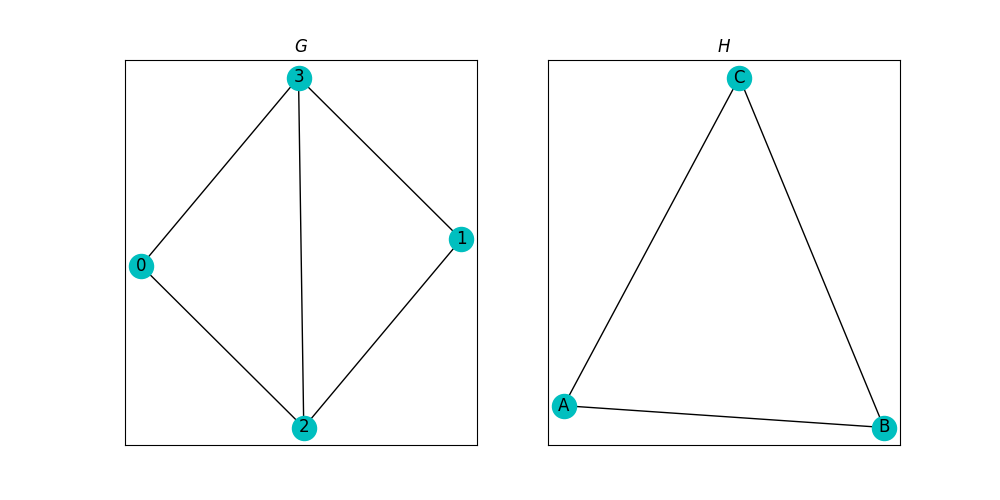
\includegraphics[width=10cm]{Images/graph_homomorphism.png}
    \centering
    \caption{A homomorphism from G to H.}
\end{figure}

For the example above we can define a mapping $f$ such that:

\begin{align*}
    &f(0) = A\\
    &f(1) = A\\
    &f(2) = B\\
    &f(3) = C\\ 
\end{align*}

$f$ is a homomorphism by the definition presented above. 
We now define particular forms of the graph homomorphism.

\begin{dfn}
    We call $f: G \rightarrow H$ an isomorphism,
 if $f$ is a homomorphism and is bijective.
\end{dfn}

\begin{figure}[h!]
    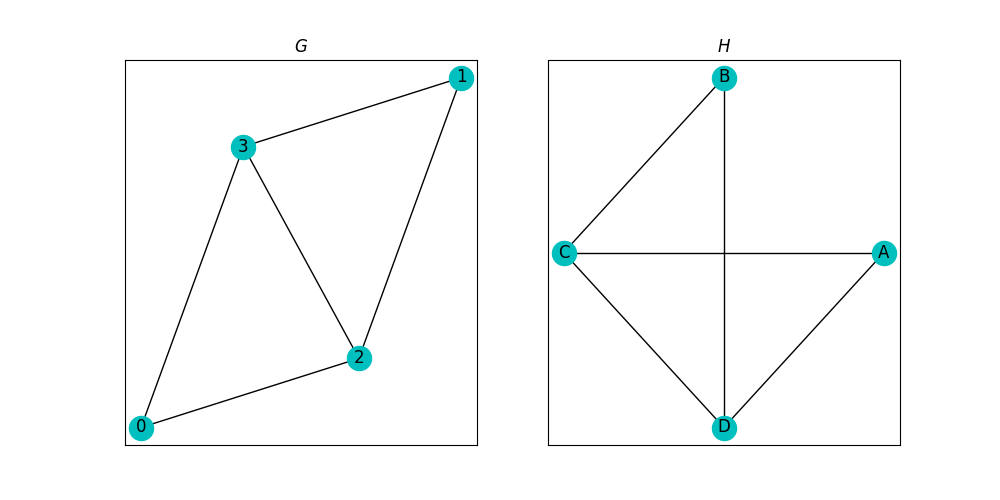
\includegraphics[width=10cm]{Images/graph_isomoprhism.png}
    \centering
    \caption{An isomorphism between $G$ and $H$.}
\end{figure}

Here we can define an isomorphism $f$ for the above figure such that:

\begin{align*}
    &g(0) = B\\
    &g(1) = A\\
    &g(2) = C\\
    &g(3) = D\\ 
\end{align*}

This is commonly referred to as an "edge-preserving bijection" as an edge between vertices $u$,$v$ for the 
graph $G$ as there exists an also an edge between vertices $f(u)$, $f(v)$ in $H$ provided that $G$ is infact
isomporhic to $H$. 

\begin{dfn}
    An automorphism is an isomorphism between a graph $G$ and itself.
\end{dfn}

The automorphism is an important distinction from that of an isomoprhism given that we we will
wish to count isomoprhisms on induced subgraphs of our networks. An automorphism of the graph
reflects it's symmetries. The set of all automorphisms of a graph $G$ is denoted $Aut(G)$ and 
the cardinailty of the set by $aut(G)$. For any graph the identity mapping is infact an isomoprhism,
but for the graph $V = \{1,2,3\}$, $E=\{(1,2),(2,3),(3,1)\}$ there exists two other automorphisms.



\begin{dfn}
    Let $G=(V,E)$ be a graph. We call $G'=(V',E')$ a subgraph if
     $V' \subseteq V \land E' \subseteq E \cap (V' \times V')$. Furthermore we call $G'$
     an induced subgraph of $G$ if for the edges $\{u,v\}$ of $G'$ we have $\{u,v\} \in V, u,v \in V'$.
\end{dfn}

Induced subgraphs are vital to our understanding of how motifs interact as we add edges or nodes
to a given graph.

\begin{figure}[h!]
    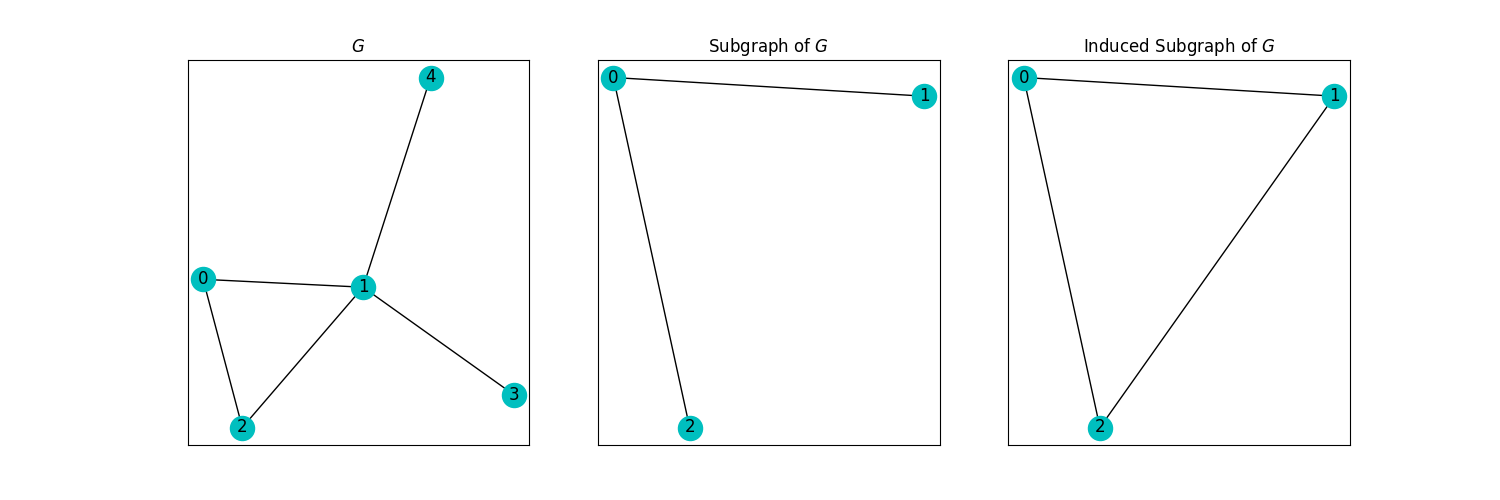
\includegraphics[width=15cm]{Images/subgraph.png}
    \centering
\end{figure}

\begin{dfn}
    Let $G'' \subset G$ and furthermore let there exist an isomorphism between $G''$ and $G'$. We call
    $G''$ an appearance of $G'$. Provided the appearances of $G'$ is greater than some $N$ we call $G'$
    a motif or pattern.
\end{dfn}

The motifs will be our focus throughout this thesis. We are interested in motif counts and how they
dynamicall evolve over time given the addition of edges and nodes. We will also seek to characterise this
devleopment using data-driven methods of analyzing dynamical systems.

\chapter{Networks}
The terms "network" and "graph" are often used interchangably as networks are often represented
via vertices and edges, but networks are graphs in a very applied context. In it's 
most general sense a network is comprised of objects and connections between those objects. These
connections may be directed, undirected, weighted representing any number of different relationships. 
For this reason we find applications of Netowrks in biology, economy, chemisty, physics, and 
many other fields. When our networks begin to approach larger scales their topological features
become considerably non-trivial. These we refer to as complex networks and they are 
commonly found in those fields mentioned above. 

Complex networks differ from other networks as edges form between vertices 
in patterns neither completly random nor regular. Such networks often have degree distributions that are fat-tailed
meaning a few nodes are of relatively high degree, while most other nodes are not. These networks
are commonly called scale-free networks. The Barabási–Albert model we examine later will fall under
this category. These networks also tend to strongly cluster, which may correlate with the scale-free 
property. For these reasons the field network theory has been gainign steadily in popularity.

\section{A Short History}

\vspace{3mm}
Networks have been a subject of accelerating interest over the last seven decades after
Paul Erdős and Alfréd Rényi developed their theory of random graphs. This 
seminal theory described a small class of networks, those of single scale. Their
random network, the Erdős-Renyi graph, was found to do well for networks of small node count 
and of simple structure, but this graph did not exhibit the scale free property that was found across so many networks
in the real world. The Erdős–Rényi graph had a degree distribution that was approximated 
well by a Poisson distribution. \cite{barabasi2016network} Paul Erdős and Alfréd Rényi's work
was absolutely critical to the beginnings of Network science, but ultimately failed to 
capture the intricacies of the real world networks. 


Their successors Réka Albert and Albert Barabási recognized that the Erdős–Rényi model 
was incapabale of modeling real world phenomena, because the Erdős–Rényi model could not add
in new nodes nor edges. Moreover all edges in the Erdős–Rényi model were added at random, but Networks
are not random per se. They conform to rules. In three key areas the real networks differed from those
simulated. \cite{barabasi2016network} First the real networks often had degreess that are not explainable according to a degree
Poisson distribution. The tail of the distribution did not allow for such things, but it was 
clearly wrong. Two - real networks often had a largest connected component - a large cluster 
of nodes inside the network, forming a hub of activity. Finally the clustering coeffecient of a network
decreases as the node size increases, but is overall independent of overall graph size.


Réka Albert and Albert Barabási began to develop a theory of complex networks that 
encompasses those networks we find common in practice. Albert and Barabási 
recognized that these complex networks are found throughout many different domains. ALbert and Barabási contended that ultimately the 
Erdős–Rényi failed to account for the dynamic growth of networks overtime, the entrance of new nodes
into the netowrk. Moreover those simple networks did not include a model of preferential attachement
as those nodes which enter the network at a new timestep prefer to attach to those nodes which are most
connected. Their model of preferential attachment was found to simulate scale-free networks well. It's use
has gained in popularity since it's inception.

Barabasi ultimately recognized some limitations in his model such as the inability to add in edges to the network
or to remove existing edges from the network. \cite{barabasi2016network} Now models are attempting to address
these short comings by introducing new mechanisms into the model, but many models still ultimately rely on
the preferential attachment mechanism formualte by Albert and Barabási.

\section{What is Twitter?}
Twitter is now, as of 2021, perhaps the preeminent example of complex network behavior in social media.
As of 2019 there are 330 millions actives users on Twitter, thirteen years after the platform was
established in 2006. However according to Pew Research the top ten percent of Twitter users tweets 138 
tweets per month, while the bottom 90 percent of Twitter users only tweet twice a month. The top ten percent
have a median 387 followers, while the bottom 90 percent have only 19 followers. The top ten percent
also follow more users, a median of 456 accounts compared to a median of 74 accounts for the bottom ninety percent \cite{wojcik2019sizing}.
This suggests highly-connected accounts drive overall dialogue and a fat-tailed
degree distribution governs both tweets produced by a user and a user's respective follower count.


\begin{figure}
    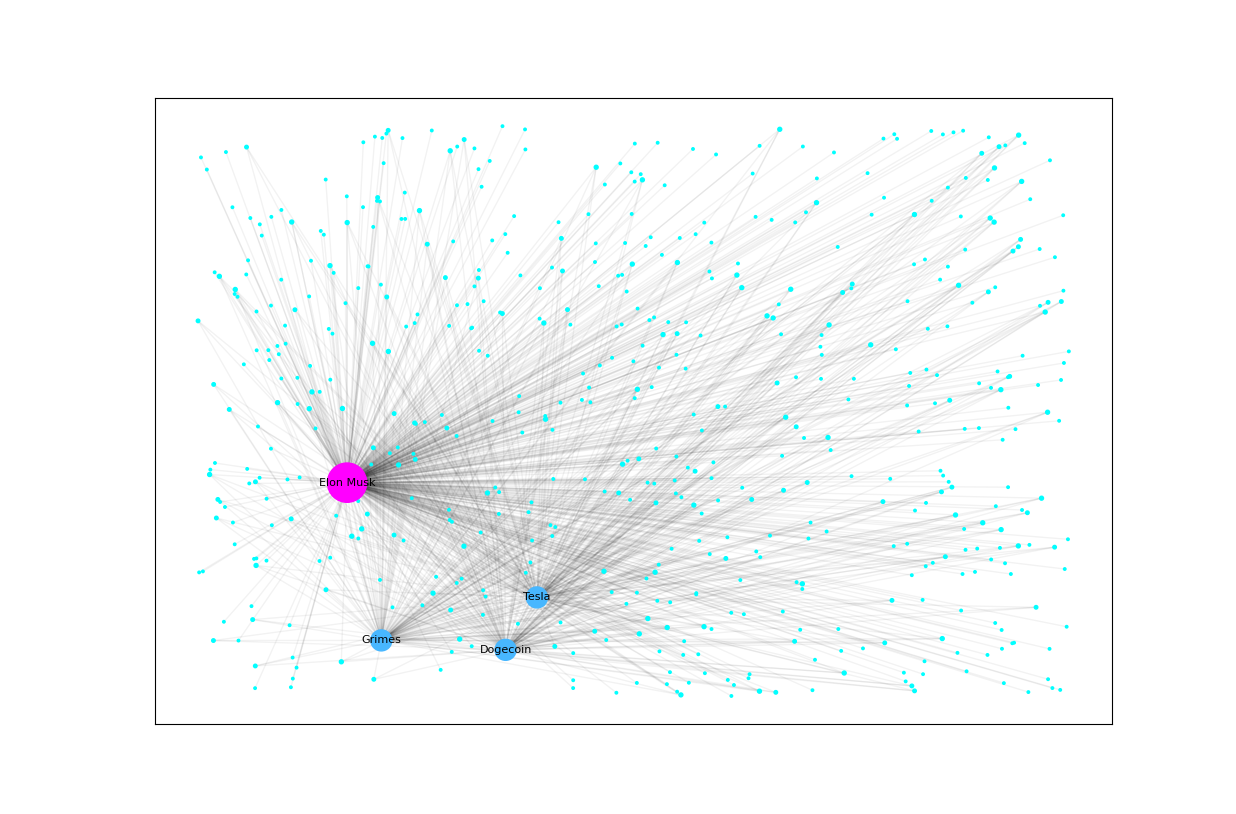
\includegraphics[width=15cm]{Images/elon_graph.png}
    \centering
    \caption{Elon Musk, as of the time of this writing, is the forty-third largest account on Twitter. With nearly 45 million
    followers, Musk can influence a wide swath of Twitter users (see Bitcoin \cite{elontweet2}, Dogecoin \cite{dogecoin}, Tesla stock price \cite{elontweet}).
    Tesla has 8.3 millions followers,
     and Grimes (Musician/Musk's Partner) has 1.1 million followers, 
     and Dogecoin has 0.6 million followers
      This graph shows a \textit{very small subset} of their followers.}
\end{figure}


Twitter is also notable for it's position among social networks not only for it's size,
but also it's influence on culture and politics. During the 2016 election, a survey of
thirty million tweets from two million users linked to articles that were found to spreading
false information. Moreover this information spread based on community structure within an inclusive left-right
influencer network. Twitter is clique-y and that communities form around 
shared interests. In online communities where exposure to the same memetic theme occurs frequently, 
facts and rumors may spread easily and \textit{very} quickly. \cite{bessi}

Twitter also carries substantial economic impact. Twitter is known to be a good predictor of Bitcoin prices
the following day. \cite{bitcoin} However only a handful of twitter users actually have influence 
although groups of people could theoretically be enought to influence market prices. \cite{stonks}
Elon Musk is one such person who as influence as of March 2021 multiple markets driving Tesla's share
price up and down, as well as the prices of cryptocurrencies. \cite{elontweet} \cite{elontweet2} \cite{dogecoin}

Twitter's suitability as a subject of Network science is clear. One can generate Networks from Twitter 
in a handful of ways. First there are the user accounts which are linked to one another through 
followers and follows, in-degrees and out-degreess. One can also construct network representations 
of network messages as discussed below in the Thij model. A user posts a message, which is then subsequently 
retweeted by a portion of their followers, which is then reweetwed by a portion of their own followers, and 
so on.

\chapter{Motifs}

Motifs are our primary object of interest as a way of characterizing the underlying substructure of a
network. We introduce motifs above, but we have yet to specify which motifs we would like to study. we
We have to discuss some motifs that are common objects of graph theory such as cycles or stars. These
will aid us in understanding the more complicated motifs introuced below. 


\section{Cyclic Motifs}

We will need terminology to discuss the dynamics of the motifs in such a way that 
makes them readily understandable. 

\begin{dfn}
    A walk $W = {v_0, e_1, v_1, \dots v_n}$ is a sequence of edges and vertices of $G$ such that
    for $0 \leq k \leq n-1$ the edge $e_i = \{v_k, v_k+1\}$.
\end{dfn}

\begin{dfn}
    A cycle is a walk whose first and last vertex are the same.
\end{dfn}

\begin{figure}[h!]
    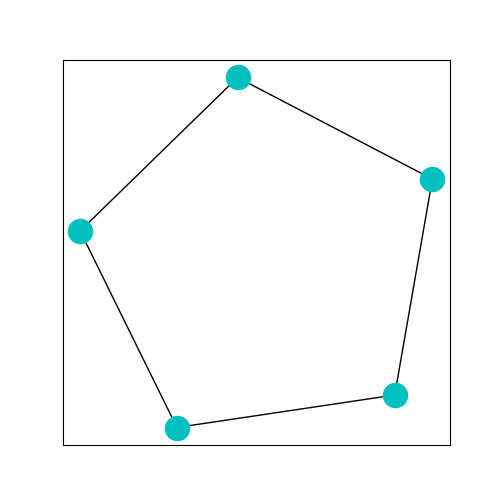
\includegraphics[width=5cm]{Images/Cycle.png}
    \centering
    \caption{A simple cycle of length 5.}
\end{figure}

We will wish to count cycles of length $k$ when count the appearnaces of more complicated motifs. When
we count cycles of length $k$ all closed $k$-walks which are not cycles will have to be subtracted. This
is relatively straightforward when using powers of the adjacency matrix as we will see later.

\begin{thm}
    Let $C_k$ be a simple cycle of length $k$. We say a graph $G$ is k-cyclic provided there exists a homomorphism $f$ such that 
    $G = f(C_k)$.
\end{thm}

\begin{dfn}
    A bipartite graph is a graph whose nodes may be separated into two disjoint sets $U$ and $V$
    such that there exists an edge between all vertices in $U$ and all vertices in $V$.
\end{dfn}

\begin{figure}[h!]
    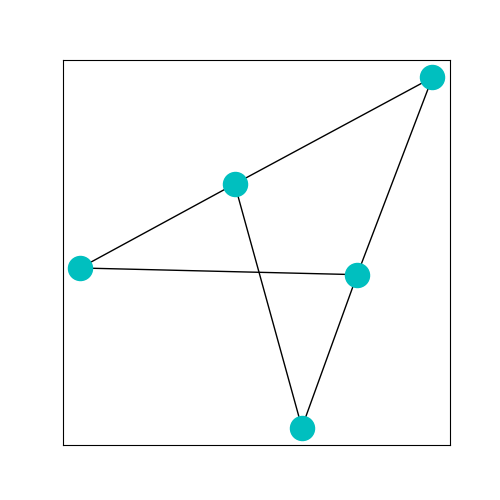
\includegraphics[width=5cm]{Images/Bipartite.png}
    \centering
    \caption{The bipartite graph $K_{2,3}$}
\end{figure}

\FloatBarrier

\begin{dfn}
    A star $S_n$ denotes the complete bipartite graph $K_{i,k}$. In other words 
    a tree with one internal node, but $k$ branches.
\end{dfn}

\begin{figure}[h!]
    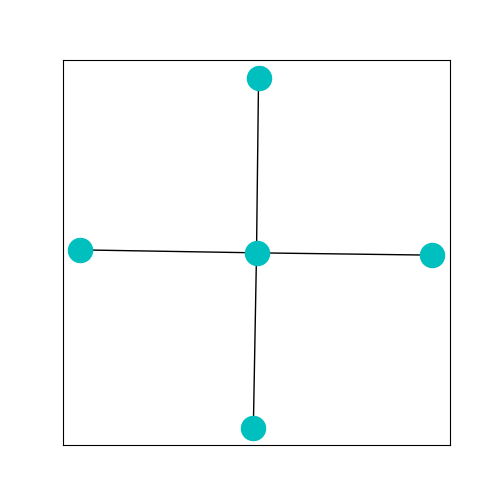
\includegraphics[width=5cm]{Images/Star.png}
    \centering
    \caption{The star $S_4$}
\end{figure}

From the statistics of each graph we can extrapolate insight into the Thij model, both 
in how it's behavior changes with respect to changes in the parameter, but also how
it differs fundamentally from the preferential attachment model described above.


\newpage

\section{Non-cyclic Motifs}

We wish to consider the following motifs: H3, H4, H5, H6, H7, H8, H9, H10, H11, H12, H13.
These motifs and the ways in which to count them are described in "Finding and Counting 
Given Length Cycles" by N. Alon, R. Yuster, and U. Zwick.


\begin{dfn}
    Let f be a homorphism between graphs $G$ and $H$. We say that $H$ is a
    homomorphic image of $G$ provided $f$ is surjective.
\end{dfn}

\begin{dfn}
    A graph $H = (V_H, E_H)$ is said to be k-cyclic, for $k > 3$, if it is a
homomorphic image of the cycle $C_k$. The number of different homomorphisms from $C_k$
to $H$ is denoted by $C_k(H)$.  $H$ is $k$-cyclic if and only if $C_k(H) > 0$.
\end{dfn}
\vspace{3mm}

For any graph below $H_k$ we could find a surjective homorphism that maps the $k$ cycle to the graph below. 
In this manner we generate the following motifs.
\vspace{3mm}

\begin{figure}[h!]
    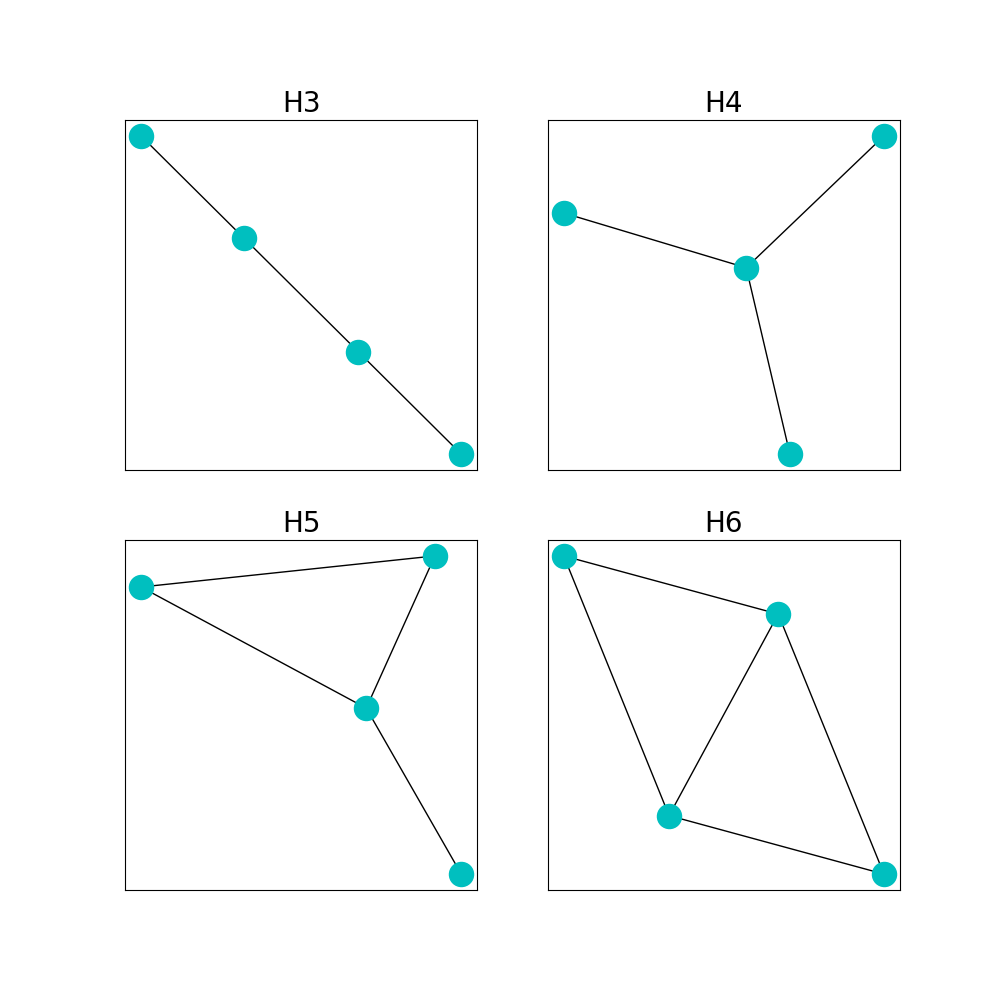
\includegraphics[width=9cm]{Images/motif_set_one.png}
    \centering
    \caption{Four non-simple motifs}
\end{figure}

\begin{figure}[h!]
    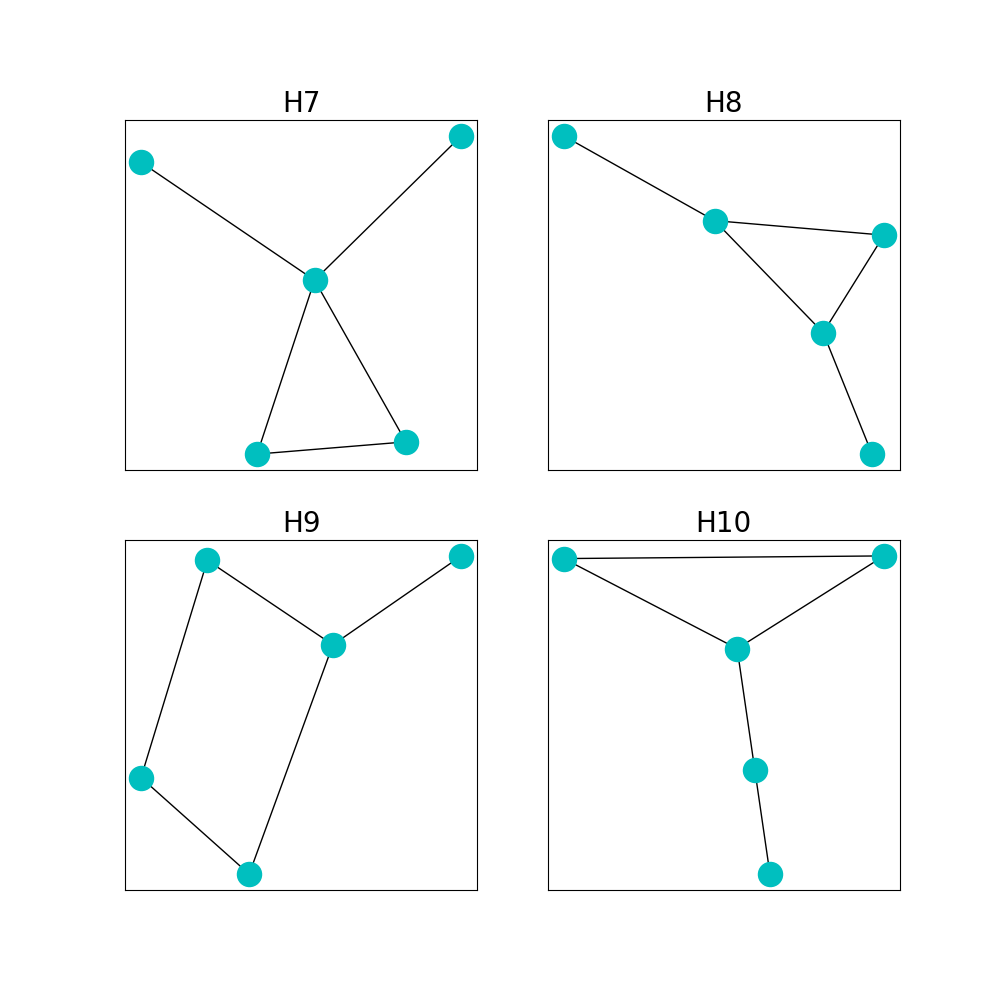
\includegraphics[width=9cm]{Images/motif_set_two.png}
    \centering
    \caption{Four more non-simple motifs}
\end{figure}

\begin{figure}
    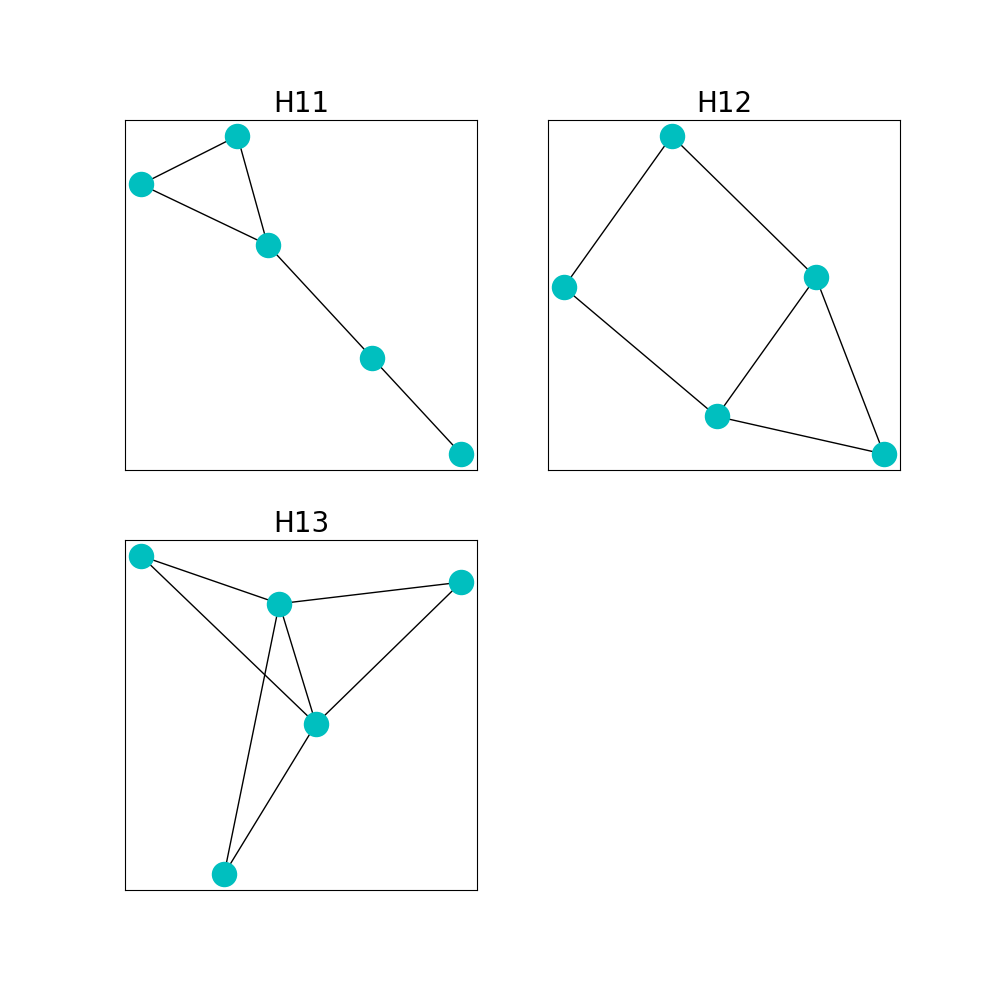
\includegraphics[width=9cm]{Images/motif_set_three.png}
    \centering
    \caption{Our last four non-simple motifs}
\end{figure}

\FloatBarrier

We may also consider walks of certain sizes as this will be necessary for 
counting appearances of each motif at any given time. Motif counts can be generated from a network's adjacency matrix in the following ways. Let $A$
be the adjacency matrix of some arbitrary network with greater than four nodes. Let $N_m(A)$ denote 
the total count of motif $m$ in the network. 

\vspace{3mm}

When counting the motifs we let $E$ denote the set of edges, $e_ij$ denotes a particular edge between the 
i'th and j'th nodes. $d_i$ denotes the degree of the i'th node. $A$ is the adjacency matrix of the 
graph $G$ with which we are concerned. Finally $a^{(k)}_{ij}$ denotes the element at the i'th row and j'th 
column of the $k'th$ power of the adjacency matrix $A$. The formulae for motif counts are as follows:

\newpage

\begin{align*}
    &N_{C3} = \frac{1}{6} \tr({A^3}) \\
    &N_{C4} = \frac{1}{8} \left(\tr(A^4) -4\sum^{n}_{i=1} {d_i \choose 2} - 2\sum_{i,j \in E} e_{ij} \right)\\
    &N_{H3} = \frac{1}{2}\sum_{(i,j)\in E} (d_i - 1)(d_j - 1) - 3 N_{C3} \\
    &N_{H4} = \sum^{n}_{i=1} {d_i \choose 3} \\
    &N_{H5} = \frac{1}{2} \sum^{n}_{i=1} a^{(3)}_{ii} (d_i-2)\\
    &N_{H6} = \sum_{(i,j)\in E}{a^{2}_{i,j} \choose 2 }\\
    &N_{H7} = \frac{1}{2} \sum^{n}_{i=1} a^{(3)}_{ii} {{d_i-2} \choose 2}\\
    &N_{H8} = \sum_{(i,j)\in E} a^{(2)}_{ij} (d_i-2)(d_j-2) - 2 N_{H6}\\
    &N_{H9} = \sum^{n}_{i-1}(d_i-2) \sum_{j \neq i} {a^{(2)}_{ij} \choose 2 }\\
    &N_{H10} = \frac{1}{2}\sum^{n}_{i=1}a^{(3)}_{ii} \sum_{j \neq i} a^{(2)}_{ij} - 3 N_{C3} - 2N_{H5} -4N_{H6}\\
    &N_{H11} = \sum^{n}_{i=1} {\frac{1}{2}a^{(3)}_{ii} \choose 2} - 2N_{H6}\\
    &N_{H12} = \sum_{(i,j)\in E} a^{(2)}_{ij} a^{(3)}_{ij} - 9N_{C3} -2N_{H5}-4N_{H6}\\
    &N_{H13} = \sum_{(i,j)\in E} {a^{(2)}_{ij} \choose 3}\\
\end{align*}



We want to understand how each of the motif counts affect one another given a certian evet occurs
in one of the simulations below. Some motifs contain induced subgraphs of the others and simple changes
to a motif may cause a combinatorial effect of new motifs appearing.

\chapter{Barabási–Albert Model}
The first model we wish to consider, and ultimately use as a base-line, is the Barabási–Albert model. The 
model is an algorithim for generating scale-free networks. We say a model is scale-free provided the 
degree distribution of the network follows a power-law. There are a few nodes with many connections and
many nodes with few connections. 


The fraction $P$ of having $k$ nodes attached for large values of $k$ is 

$$
P(k) \approx k^{-\gamma} , \quad 2< \gamma <3
$$

Moreover we can therein see the scale-free proprty as any scaling $c$ of $k$ gives a porportional scaling
by $c^{-\gamma}$.

We first begin at $t=0$ by initializing a $m$ number of nodes and randomly distribute a number of edges between them.
Then at each time-step $t > 0$ we introduce a new node and a $k$ number of edges between that node 
and a $k$ number of existing nodes. We assign probabilities of attachment via 

$$
P(n) = \frac{d_n}{\sum^{N}_{i=1} d_i}
$$

where $d_i$ is the degree of the i'th node and $N$ is the total number of nodes at $t-1$ the previous time-step.


Taking $m=2$ and $k=2$ we can visualize the development of the graph.

\begin{figure*}[h!]
    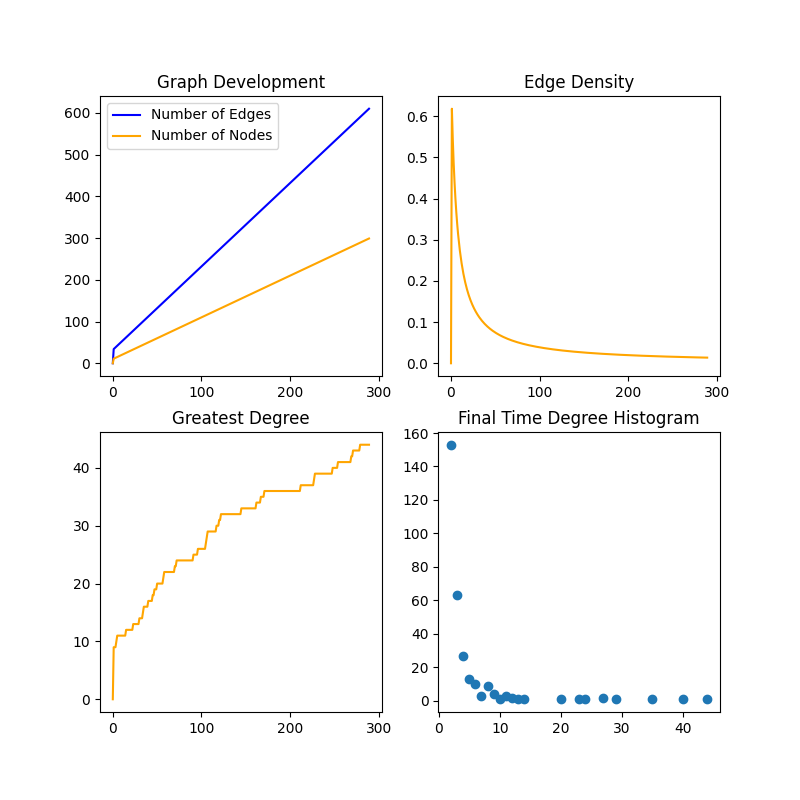
\includegraphics[width=10cm]{Images/graph_stats_pref_attach_10_2_300-210118-163357.png}
    \centering
\end{figure*}

\begin{figure*}[h!]
    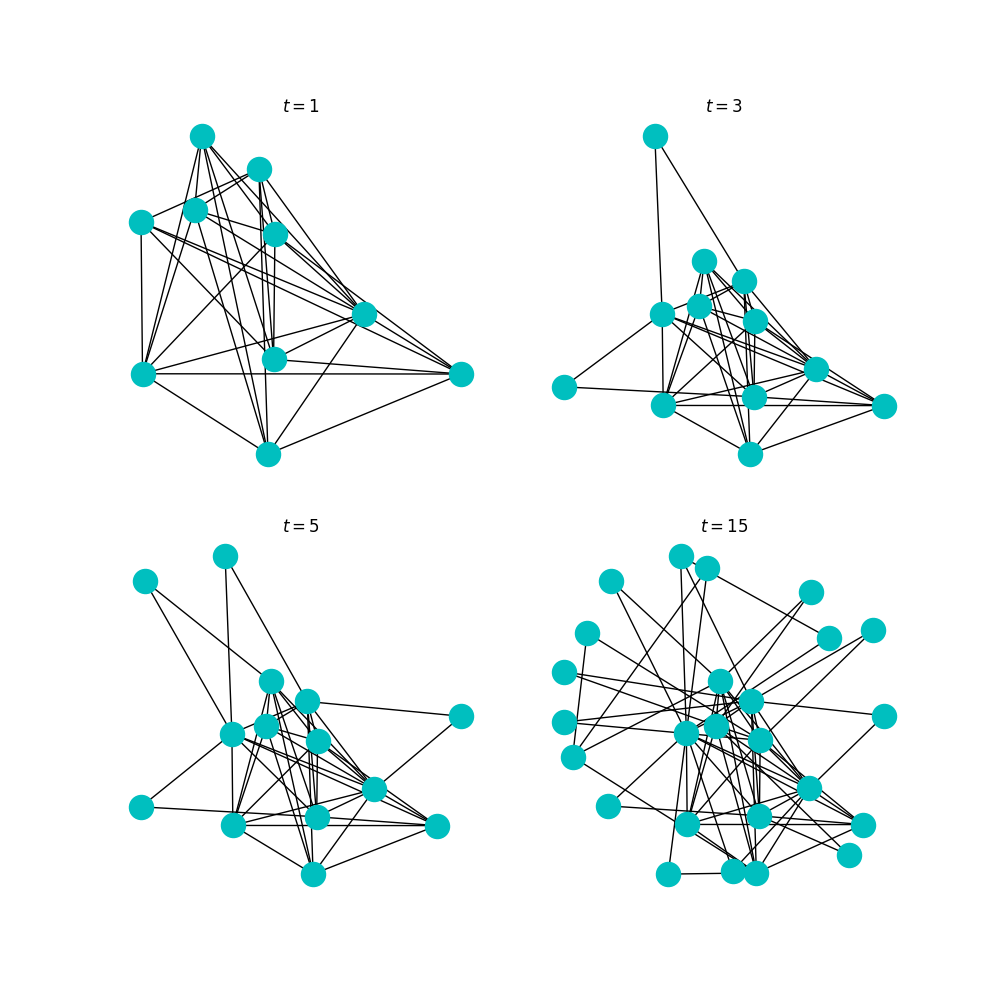
\includegraphics[width=10cm]{Images/early_graph_data210118-163357.png}
    \centering
\end{figure*}

The Barabási–Albert model exhibits a few characteristics that differentiate it from the 
Erdős–Rényi model. If we consider it's diameter, the maximum distance in the network
for $m>1$ and sufficiently large time we can write the diameter 

$$\text{diam}(G) = \frac{\ln(n)}{\ln\ln N}$$

The diamter grows slower than $\ln n$ meaning the graph's diameter grows slower than that of the 
Erdős–Rényi model. We can also examine the clustering coeffecient of the model. 
The clustering coeffecients for the preferentiall attachment model grows according to

$$
C(G) = \frac{(\ln N)^2}{\ln N}
$$

This differs from the Erdős–Rényi model by the term $(\ln N)^2$,
which increases the clustering coefficient for large $N$.
The  Barabási-Albert  network  is  locally  more  clustered  than a random network.


The model itself is a good candidate to compare to the Thij model given that Thij model incoporates
a preferential attachment mechanism itself, but is slightly more complex. The Barabási–Albert model 
represents a simpler non-trivial model which is widely acknowledged as a useful tool
for understanding networks across a variety of disciplines. We should however note the 
limiatations to the Barabási–Albert model. The nodes and edges are restricted to growing linearly which
may fail to capture certain phenomena that appears empirically. The model is also incapable 
of removing nodes, a point on which Barabási himself has elaborated on.

\chapter{Twitter and the Thij Model}
The Thij model is a particular random graph that seeks to model the behavior in which a Twitter network 
develops. \cite{thij}  Twitter is a social media platform in which a user, as of the current date, may post a message
to all of their followers' feeds. Those followers may then ignore, like, or retweet that message. In the
instance they choose to retweet the message, that message is then posted to their respective timeline and a 
new set of followers now has the opportunity to then retweet that same message. It is easy to infer that if a 
message has recieved a significant number of retweets, then the message is more likely to be seen, and thus
retweeted again. We suspect a preferential attachment mechanism driving popularity of the most popular tweets.

However a user can retweet different orignal messages at different times meaning edges are generated between
existing nodes in the network. Accounting for this one can produce
a model better suited to twitter than the Barabási–Albert model described above. In 2014 Marijn Ten Thij
and his coauthors developed the following Twitter Model.

We begin with an inital message node $n$ at time $t=0$. There is now the possibility of three events: $T1$,
$T2$, and $T3$.

\vspace{3mm}
$T1$: A new message node from user $u$ appears.

\vspace{3mm}
$T2$: A user $v$ enters the network and retweets an existing user $u$. This user $v$ retweets the original message node with 
probability $q$ and another node with probability $\frac{1-q}{N}$, $N$ being the total number of non-message nodes.

\vspace{3mm}
$T3$: An existing user $v$ retweets another existing user $u$. Once again the retweeter retweets a message node with probability 
$q$ and all other non-message nodes with probability $\frac{1-q}{N}$.

\vspace{3mm}

We must also note that generally there will be multiple message nodes in the retweet graph, and thus we have to decide for any given event
which particular message node should be retweeted. Here we introduce a preferential attachment mechanism. Thus at any time $t$
given a $T2$ or $T3$ event occuring the probability of a particular message node being chosen by others is almost the
same mechanism described in the Barabási–Albert model above. Instead a message node is chosen
by the total number of descendants it has, not by the degree itself. In essence a message node
is selected based upon the number of those who have retweeted the message, and all those who have retweeted
retweets. 

Let $\lambda \geq 0$ and $1 \geq p \geq 0$,
\begin{align*}
    &P(T1) = \frac{\lambda}{1 + \lambda} \\
    &P(T2) = \frac{p}{1 + \lambda} \\
    &P(T3) = \frac{1-p}{1 + \lambda} \\
\end{align*}


\begin{figure*}
    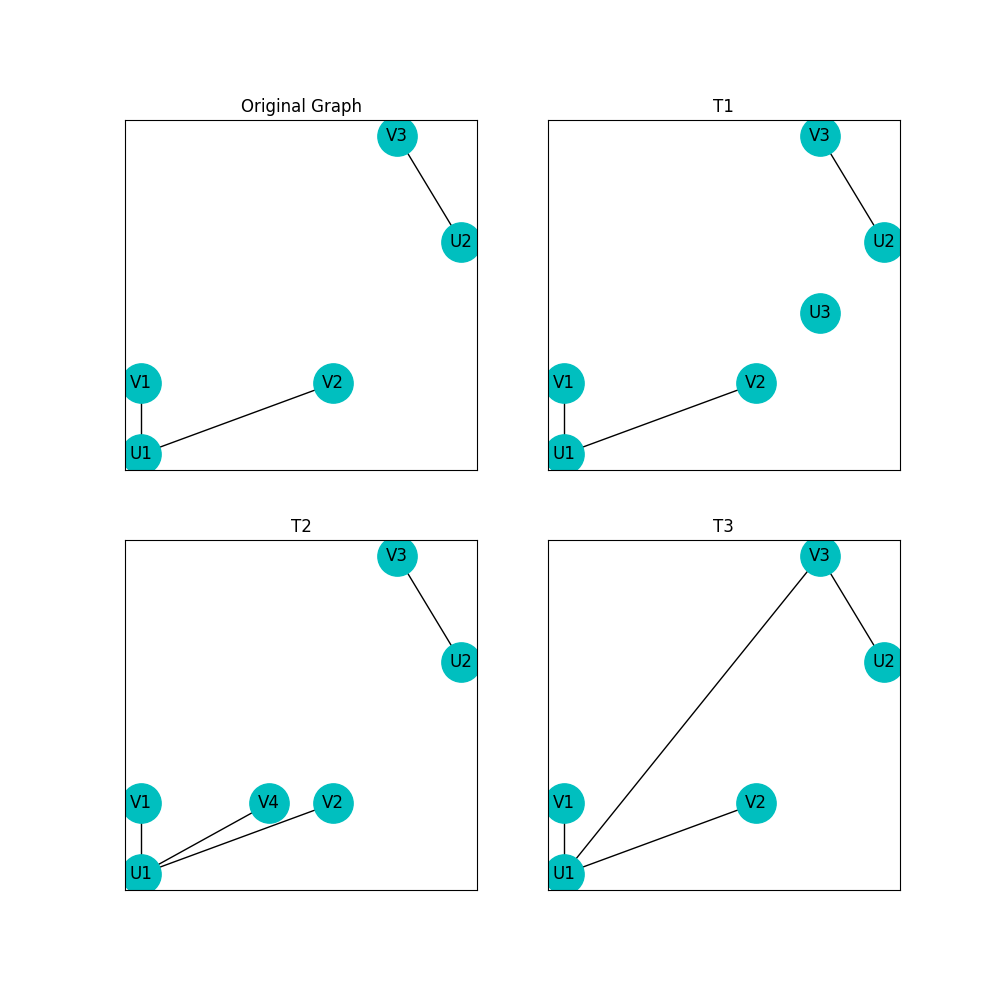
\includegraphics[width=10cm]{Images/events.png}\
    \centering
\end{figure*}
\vspace{3mm}

Our choices of $\lambda$ and $p$ will drastically affect the dynamics of the graph, as well as the subgraph motifs that will
occur. We want to consider a series of cases for different probabilities allowing us to make informed predictions about the devlopment
of the graph over time.

\begin{figure}[h!]
    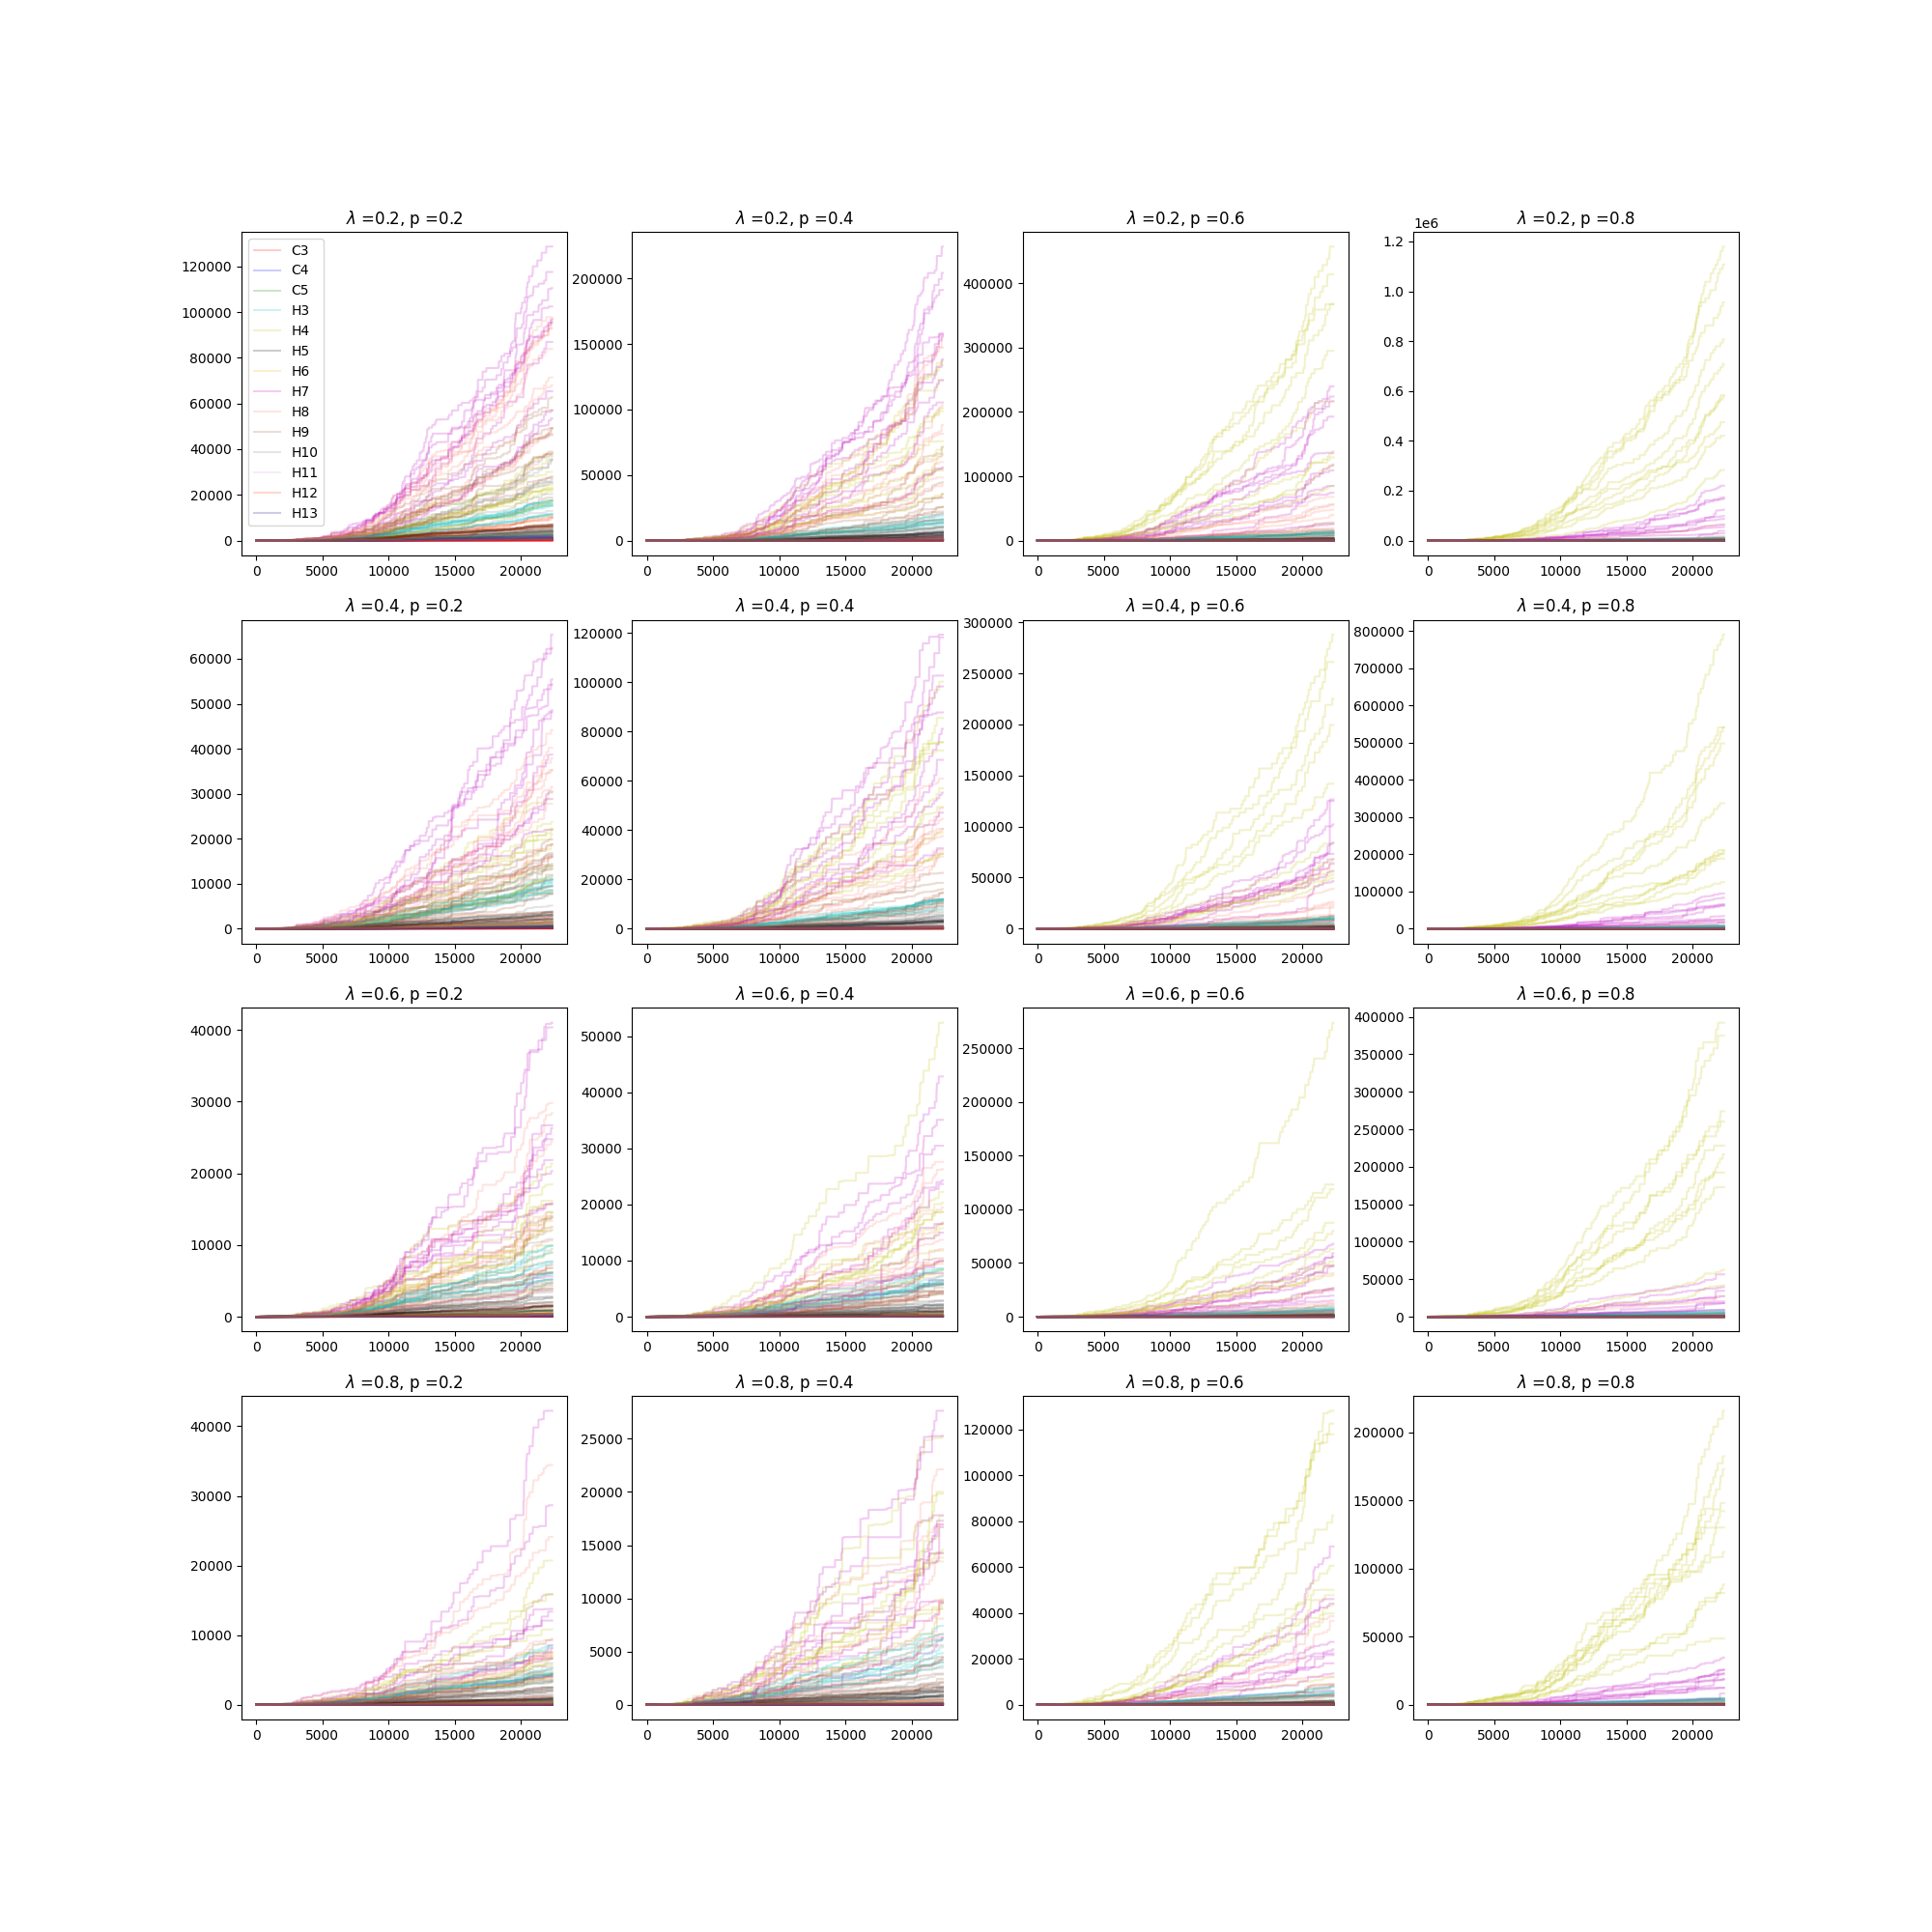
\includegraphics[width=10cm]{Images/full-sims-graph_mid_set.png}
    \centering
    \caption{Motif Counts for varying parameters. The scales on the y-axis differ widely,
    but we also see prominence of different motifs dependent upon the parameter choices. 
    Some paramters lead to large induced star subgraphs, while others may lead to 
    highly clustered communities that may share a few connections between their nodes.}
\end{figure}
\newpage

\vspace{3mm}

The motif counts for various parameters help demonstrate the differences that arise. 
Consider $\lambda>0.5$ and $p>0.5$ we see that there is an increased chance of adding
many new root messages, but still a good possibility of introducing a new node with a new edge,
or a new edge between existing nodes. $0<\lambda<0.5$ and $p>0.5$ means that adding a new node
with a new edge is the most likely outcome. The superstar probability $q$ means that these
are very likely to attach to a root message node. The preferential attachment mechanism then
encourages an induced subgraph $S_{k}$ to form with $k>>1$. For any $k\geq3$ $S_{i,k}$
itself has many appearences of $H4$ and for every increase in $k$ we see an increase in the probability
of yet another increase in $k$. On the graph above we can see this phenomena clearly with $H4$
dominating the motif counts for high $p$-values.

\vspace{3mm}
Next consider $\lambda>0.5$ and $0.5>p>0$. Here the $T1$ event should dominate the dynamics 
with many new message nodes being introduced to the overall retweet network. However these
message nodes may only contribute to the overall motif counts provided more than 2 $T2$  events
attach nodes to them or they become attached to some other node through a $T3$ event.
Last we consider the case when $0.5>\lambda>0$ and $0.5>p>0$. In this case it is the $T3$ 
that is expected to be the most prevalent. We know expect connections to form between any two nodes. Given
the superstar attachment nodes should overwhelmingly be attached to atleast one message node, and may attach 
to each other thus forming a simple three-walk. This generates many $H7$'s and $H8$'s as we can
see in the graphs above.

\vspace{3mm}

If we examine the graphs development for a few different pairs of parameters we can gain some statistical insight that
will inform how each graph is developing.

\subsection*{$\lambda=0.2$, $p=0.2$}

\begin{figure*}[h!]
    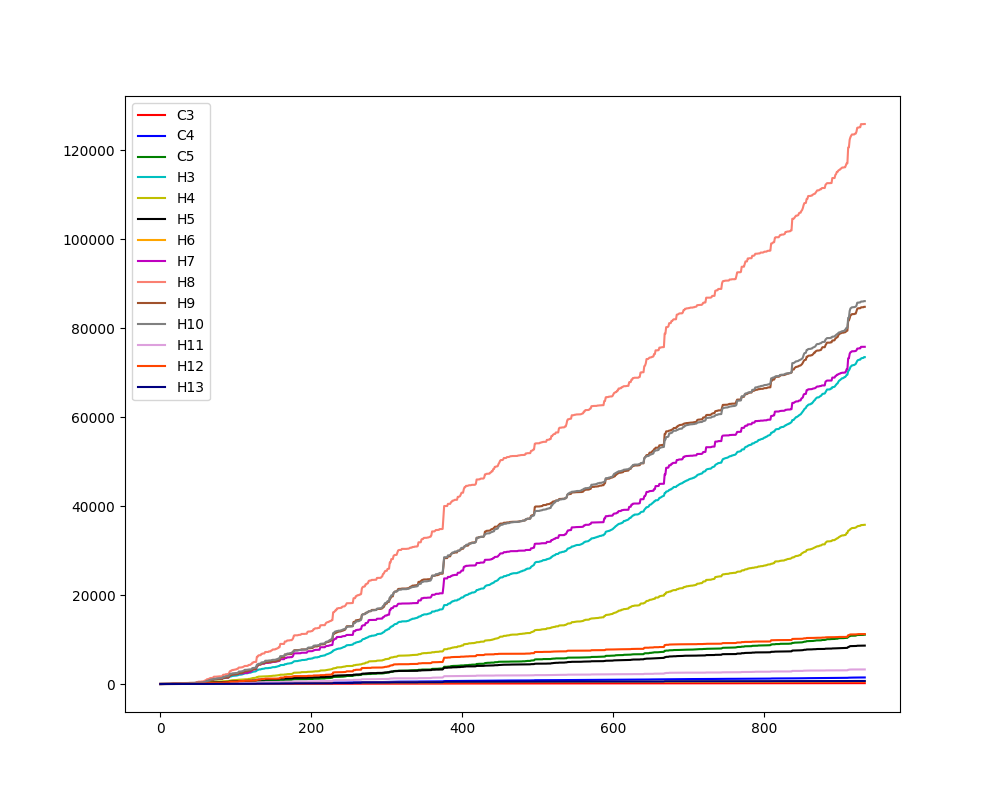
\includegraphics[width=8cm]{Images/twitter_sim_for_stats_3_0.2_0.2.png}
    \centering
\end{figure*}

\begin{figure*}[h!]
    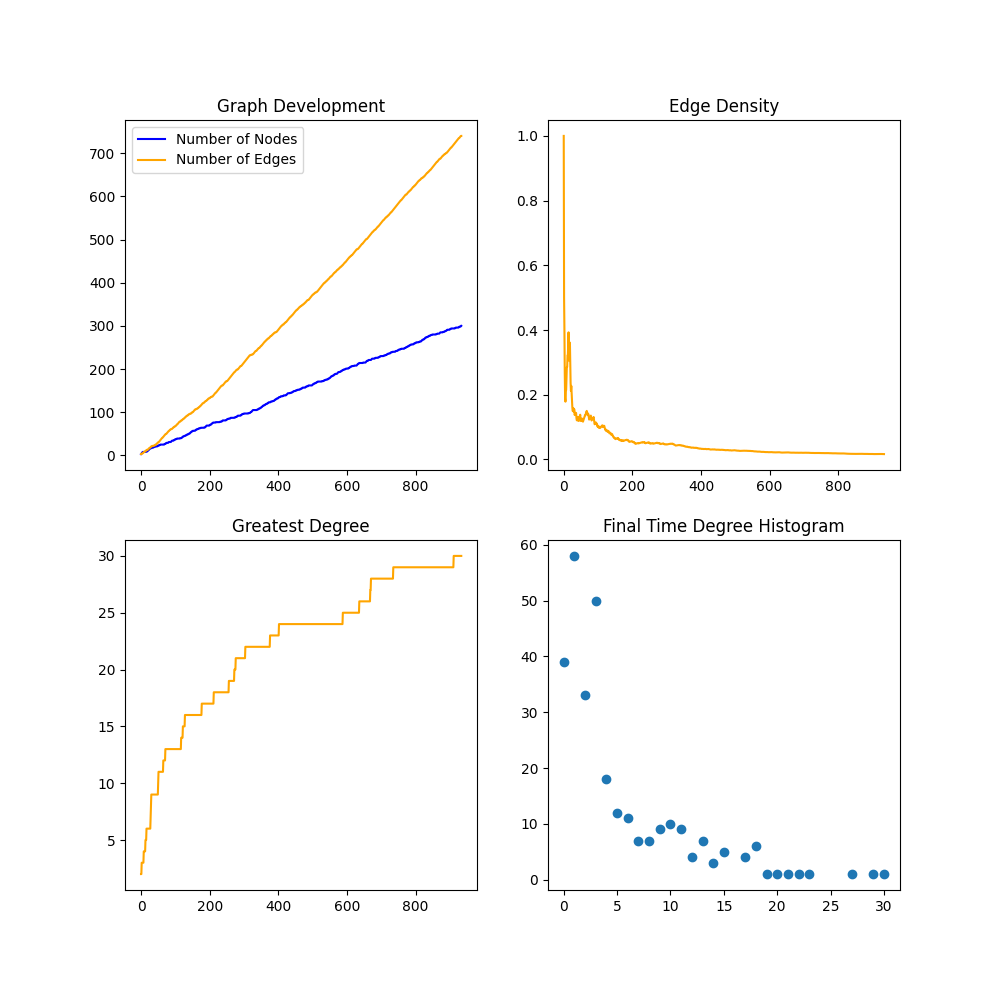
\includegraphics[width=8cm]{Images/twitter_sim_stats_3_0.2_0.2.png}
    \centering
\end{figure*}

\FloatBarrier

\subsection*{$\lambda=0.8$, $p=0.2$}

\begin{figure*}[h!]
    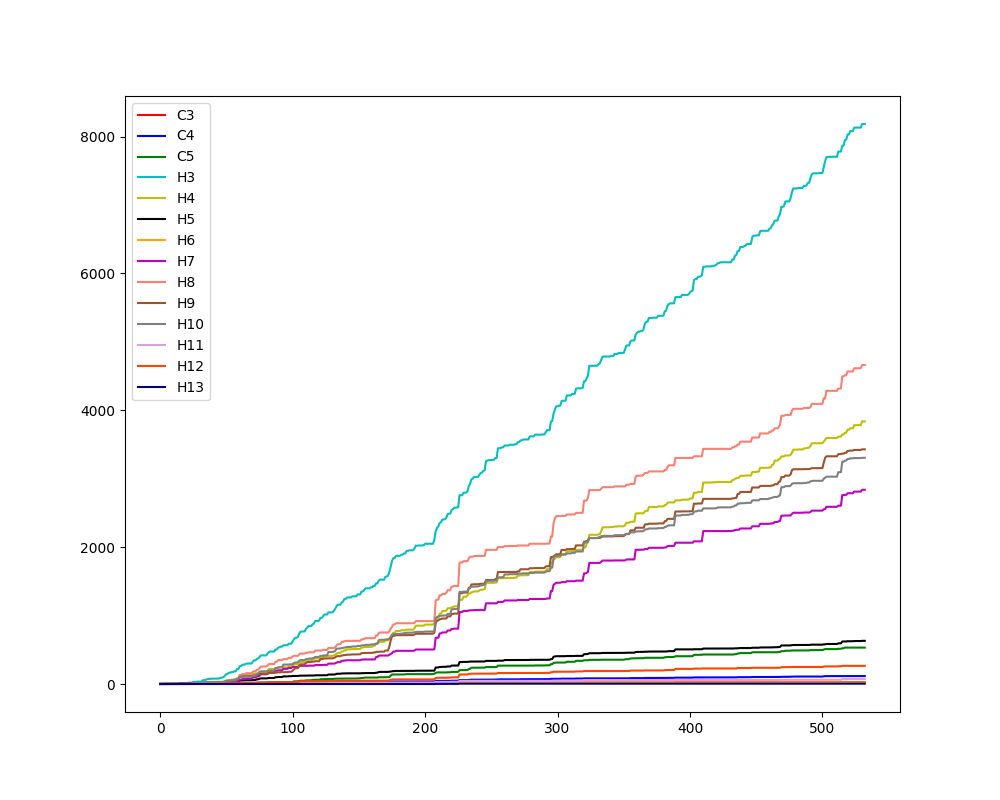
\includegraphics[width=8cm]{Images/twitter_sim_for_stats_3_0.8_0.2.png}
    \centering
\end{figure*}

\begin{figure*}[h!]
    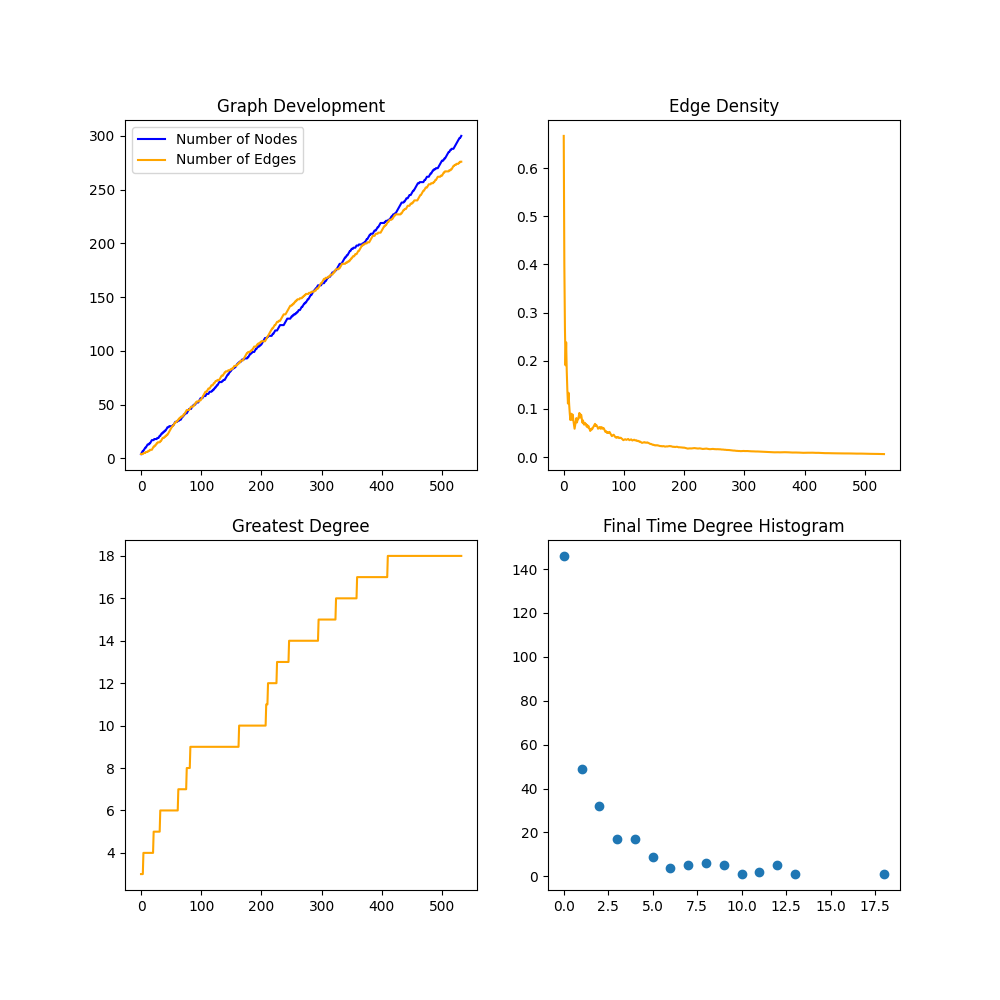
\includegraphics[width=8cm]{Images/twitter_sim_stats_3_0.8_0.2.png}
    \centering
\end{figure*}

\FloatBarrier

\subsection*{$\lambda=0.2$, $p=0.8$}

\begin{figure*}[h!]
    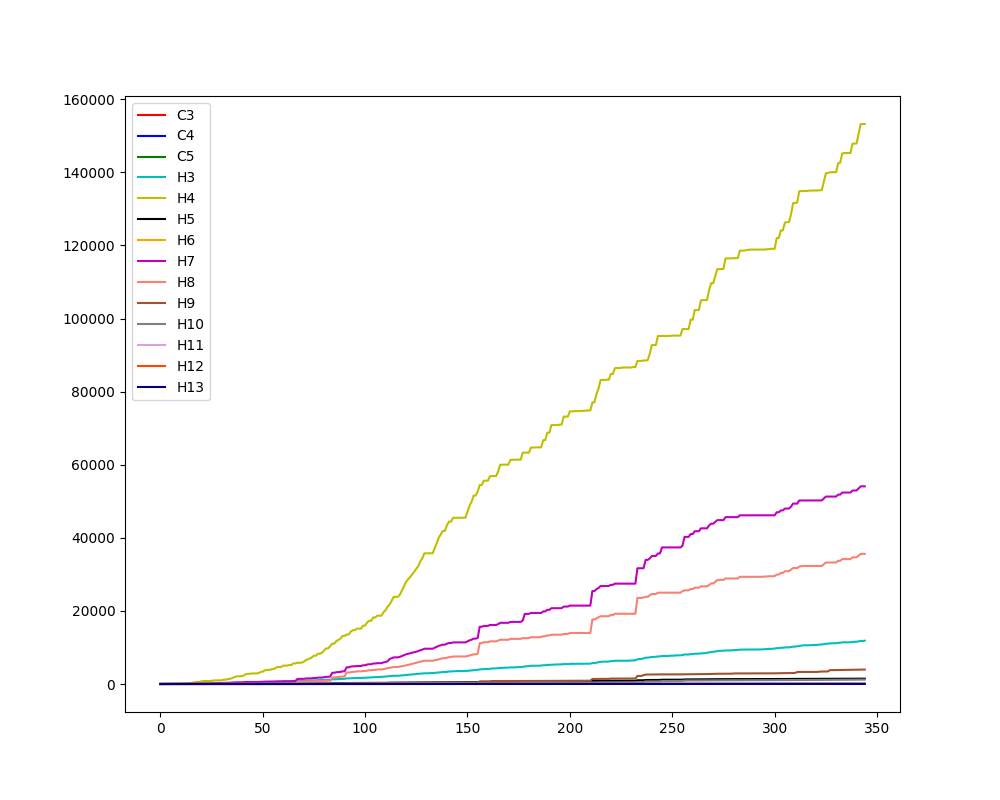
\includegraphics[width=8cm]{Images/twitter_sim_for_stats_3_0.2_0.8.png}
    \centering
\end{figure*}


\begin{figure*}[h!]
    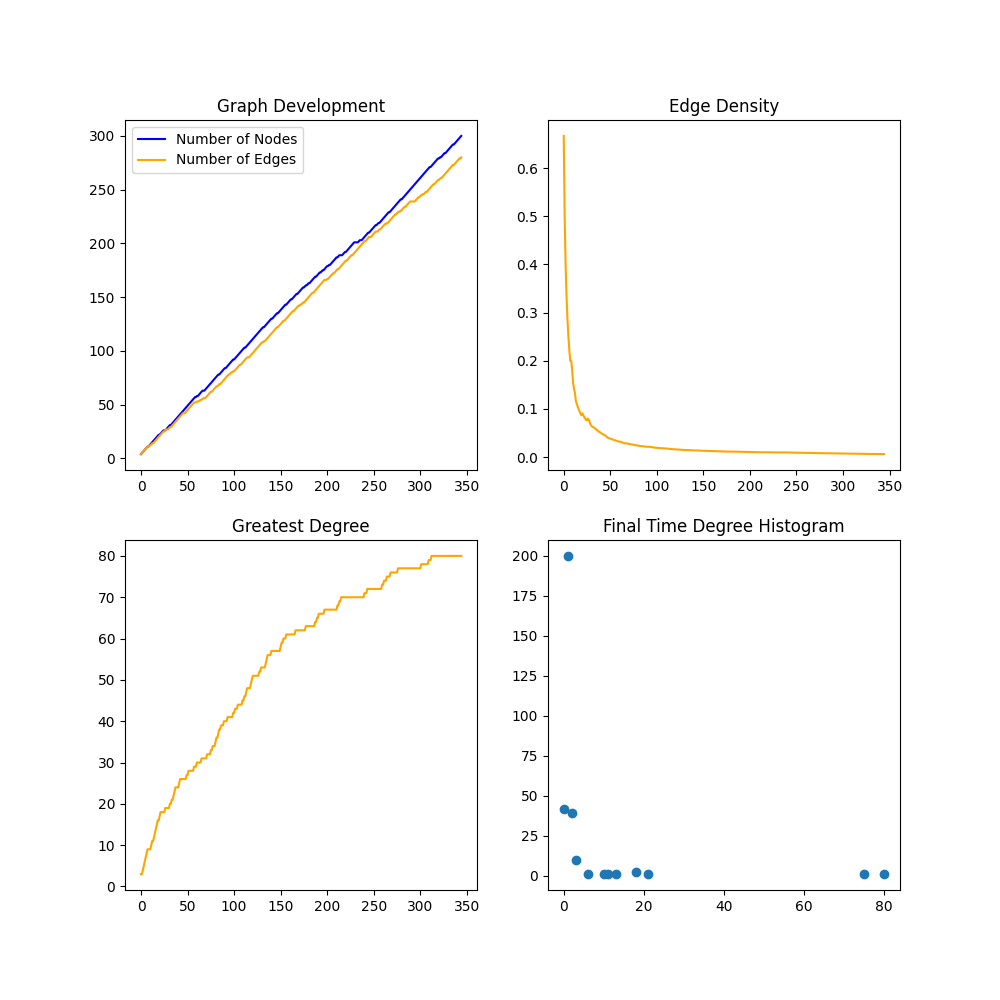
\includegraphics[width=8cm]{Images/twitter_sim_stats_3_0.2_0.8.png}
    \centering
    \caption{Here we see a two nodes with degrees greater than 70,
    but an abundnace of nodes with only one or two connections. This suggests
    two large star graphs focused around two heavily connected nodes. This 
    would produce the abundance of $H8$'s we see in the motif counts above.}
\end{figure*}

\FloatBarrier

\subsection*{$\lambda=0.8$, $p=0.8$}

\begin{figure*}[h!]
    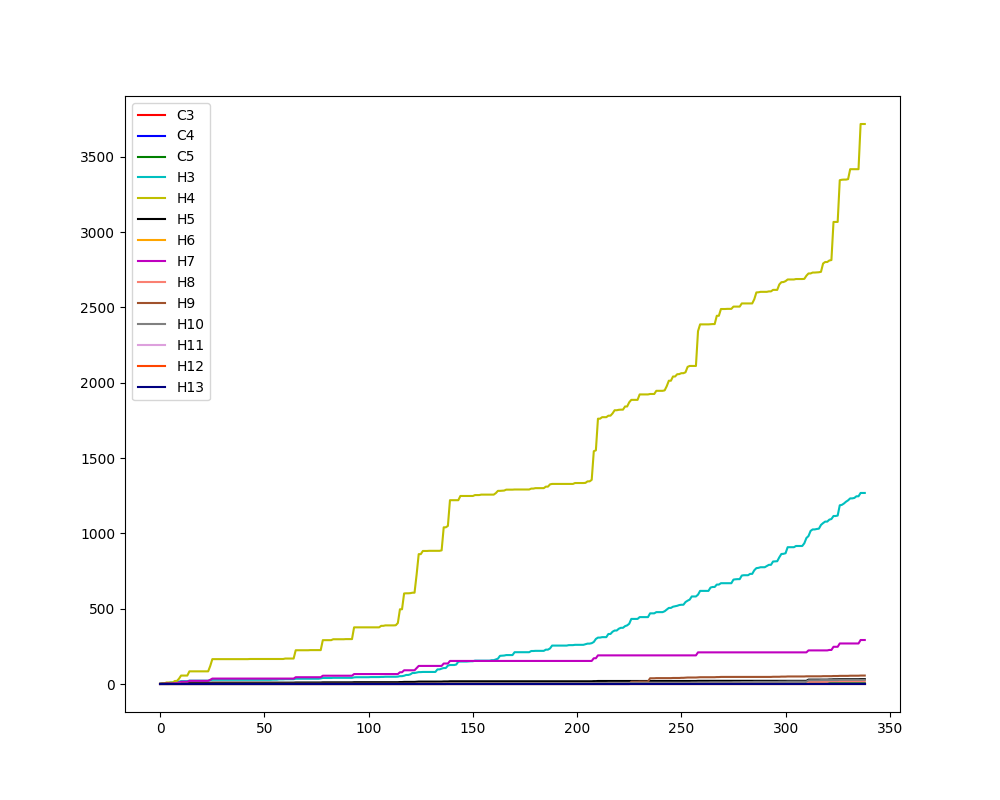
\includegraphics[width=8cm]{Images/twitter_sim_for_stats_3_0.8_0.8.png}
    \centering
\end{figure*}

\begin{figure*}[h!]
    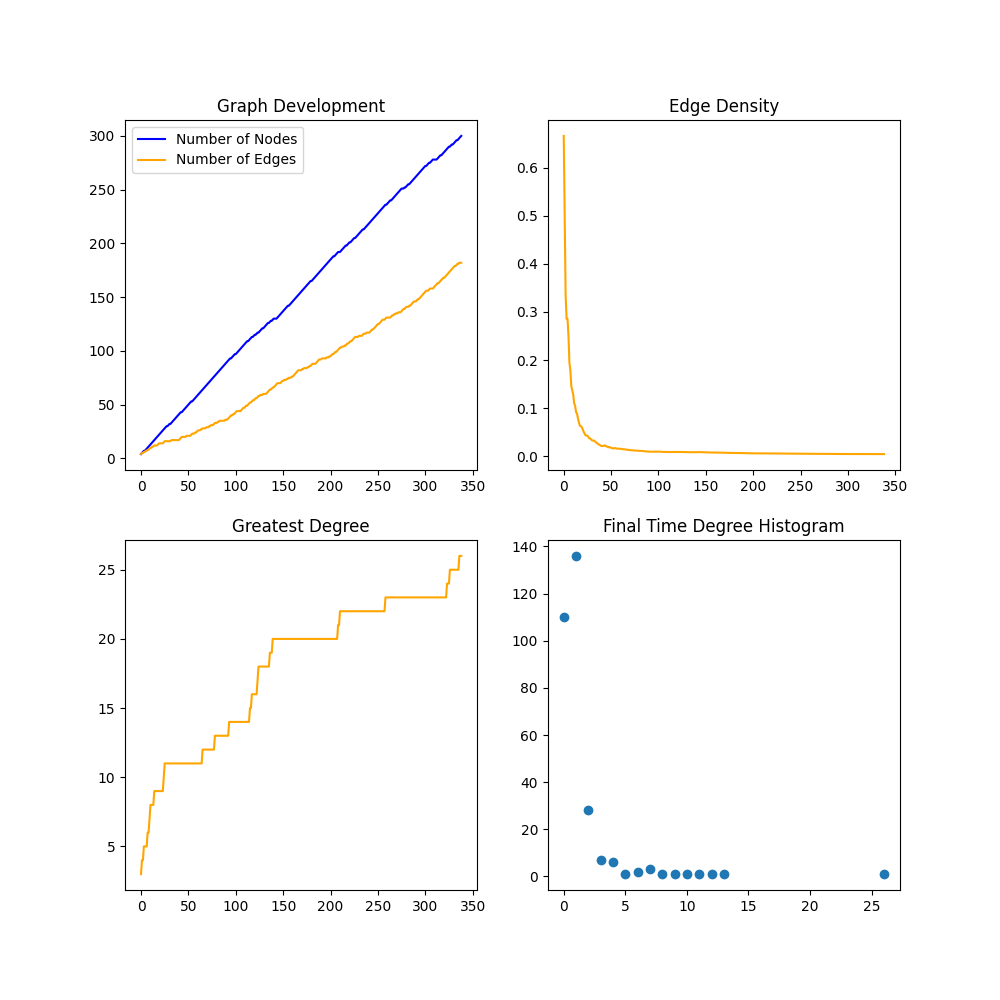
\includegraphics[width=8cm]{Images/twitter_sim_stats_3_0.8_0.8.png}
    \centering
    \caption{This twitter simulation produces many more nodes than 
    edges because of the frequency of $T1$ events. The vast majority of nodes only 
    have degrees of one or two, while we see a single node with 25 connections.
    This might suggest many small clusters of nodes with a single larger
    cluster around a single message node.}
\end{figure*}

\FloatBarrier

We see that both the dynamics and ultimately the end state vary across parameter choices.
For certainy values of parameters we see that the degree distribution will obey stronger
power laws with the vast majority of the nodes having very few connections, while a few may hold
perhaps double or triple the number of connections of any other node. We also see that
the ratio of edges to vertices for the Twitter model varies much more than the Barbási-Albert model
which is to be expected given the probabilistic nature of how many edges may be added in a given turn (0 or 1) compared
to the given $m$ of the Barabási–Albert model.

\vspace{3mm}

It should also be noted that each graph spans over \textit{very} different
time frames. Each graph was allowed to grow to a maximum of three-hundred nodes, same as the
sampled Barabási–Albert run. For $\lambda=0.2$ and $p=0.8$ the model was able to reach 
three-hundred nodes very quickly in little over three-hundred whereas for $\lambda=0.2$ and $p=0.2$ it took nearly a thousand time
steps. This is to be expected a $\lambda$ controls how often a new node enters without a new edge and
$p$ controls the rate at which new nodes are added without attached edges or if only new edges are introduced. 

\vspace{3mm}

We should remark that the concept of a superstar attachment mechanism should be attributed to Shankar 
Bahamdi and his coauthors who first proposed the mechanism in 2015 \cite{Bhamidi_2015}. Above
we see the superstar mechanism in the parameter $q$ which dictates how given a tree is selected an edge
is added to a root mode, an orignal message, or a retweet of that message. Bahamadi showed that the 
mechanism itself influenced the asymptotic development of the network's qualities. Given the modifications that
Thij has made in his model these rules may only apply to message trees within the Thij model, but they
are worth considering.

\chapter{Preferential Attachment Model Motif and Thij T2 Event Motif Dynamics}
The preferential attachment model grows by adding a node at each time step and then
attach an $m$ number of nodes at each time step. If $m$=1 this is a twitter sim
with probability one for a $T2$ event. In the simulations we consider $m=2$ which allows
for the possibility of cycles to occur similar to what we see in the Thij model. Below we 
lay out how a motif changes given a new node is attached some existing node in the motif. We 
consider these events up to symmetry. This description will also suffice for a glimpse into how the $T2$ mechanism in the Thij
model works. Later we will discuss the possibbilities that arise from $T3$.

\section{H3}
We begin by considering the $H3$ motif: Four nodes, with only three edges whose source node is the same
node, but the target node is unique. The middle node is most heavily connected, and thus is most likely
to be attached to in preferential attachment. With a single $H4$ the probability for attachment to this
center node is $0.5$. For any other node the probability is $16.67$. 


Suppose we attach to the most connect mode. We've now generated another $H4$. This increases the probability
of another node being attached to the center at the next event, and if another node is attached 

\begin{figure}[!ht]
    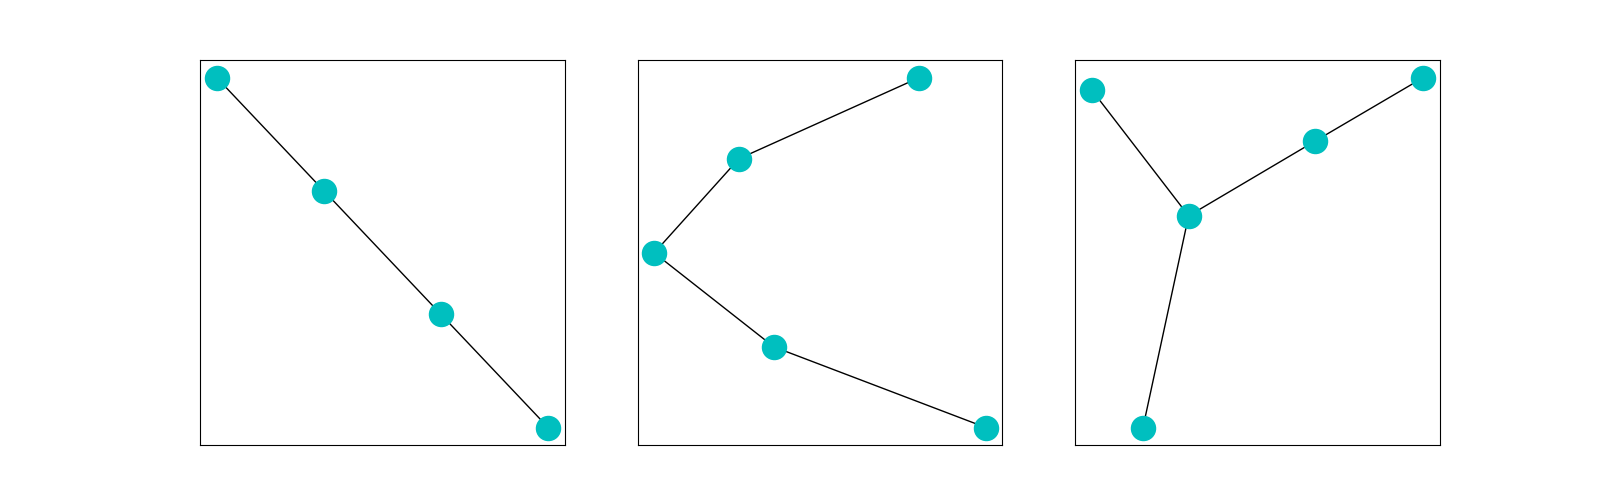
\includegraphics[width=10cm]{Images/H3_evolution.png}
    \centering
\end{figure}
\FloatBarrier



\begin{table}[h!]
    \centering
        \begin{tabular}{||c c c c||} 
            \hline
            Motif Count & Original Motif & Event 1 & Event 2\\ [0.5ex] 
            \hline\hline
            H3 & 1 & 2 & 2\\ 
            \hline
            H4 & 0 & 0 & 1\\
            \hline
        \end{tabular}
        \caption{Variations of the $T2$ event on the $H3$ motif}
        \label{table:1}
\end{table}

\section{H4}
The $H4$ motif is one of the motifs that are of primary interest given that for any star $S_k$
with $k \geq 3$ we will find many appearances of $H4$ motifs specifically ${k \choose 3}$ motifs. For large
clusters of $H4$ motifs the $H4$ motif count will grow very rapidly in time. The probability 
for an event one on the single motif is $0.5$, and for the event two $0.5$. However a siginificant
difference in the occurence of event ones over event twos will encourage more event ones in the future. 


\vspace{3mm}

\begin{figure}[!ht]
    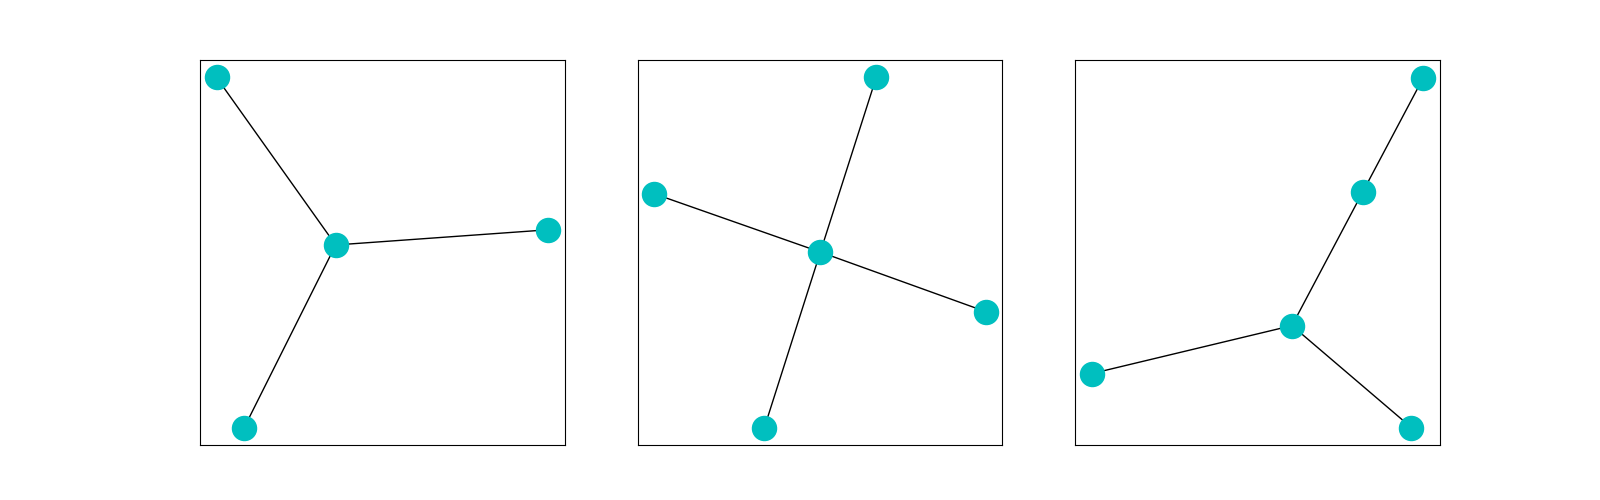
\includegraphics[width=10cm]{Images/H4_evolution.png}
    \centering
\end{figure}

\begin{table}[h!]
    \centering
    \begin{tabular}{||c c c c||} 
    \hline
    Motif Count & Original Motif & Event 1 & Event 2\\ [0.5ex] 
    \hline\hline
    H3 & 0 & 0 & 2\\ 
    \hline
    H4 & 1 & 4 & 1\\
    \hline
    H5 & 0 & 0 & 0\\
    \hline
   \end{tabular}
   \caption{Variations of the $T2$ event on the $H4$ motif}
    \label{table:2}
\end{table}


\FloatBarrier


\section{H5}
H5's are of interest due the relationship they carry to the $H4$ motif and the 
$H7$ and $H8$ motifs. The $C_3$ cycle in the motif makes the $H5$ motif isomorphic to
an induced subgraph of the $H7$ and $H8$ motifs meaning a priori we expect them to correlate. We 
also see the $H4$ is isomorphic to an induced subgraph of the $H5$. The relationship between
$H4$ and $H5$ will be explored in depth for our $T3$ analysis. The probabilities are as follows:



\begin{figure}[!ht]
    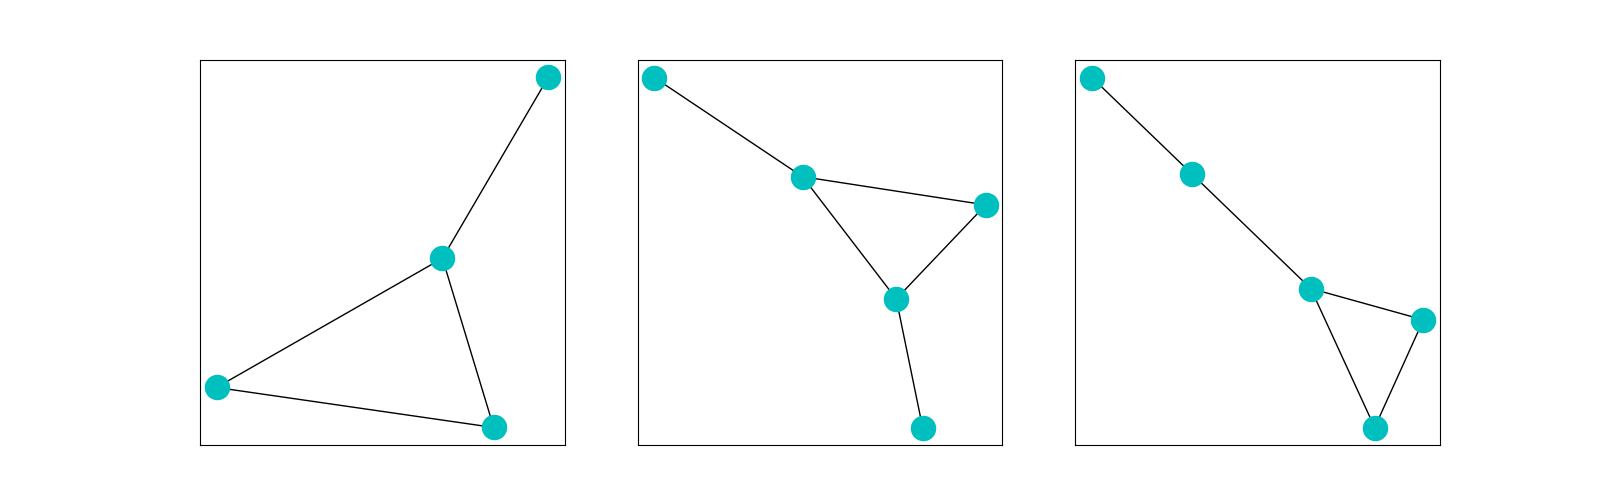
\includegraphics[width=10cm]{Images/H5_evolution.png}
    \centering
\end{figure}
\FloatBarrier

\begin{table}
    \centering
    \begin{tabular}{||c c c c||} 
    \hline
    Motif Count & Original Motif & Event 1 & Event 2\\ [0.5ex] 
    \hline\hline
    H3 & 2 & 4 & 4\\ 
    \hline
    H4 & 1 & 2 & 1\\
    \hline
    H5 & 1 & 2 & 1\\
    \hline
   \end{tabular}
   \caption{Variations of the $T2$ event on the $H5$ motif}
    \label{table:3}
\end{table}


\section{H6}
The $H6$ motif is formed by an H4 with two edges between the three outer nodes.
The $H6$ motif count is not relatively high when compared to other motifs in the Thij
model because it would require exact pairs of $T3$ events to generate them. Morever this
$T3$ event has to occure between what are likely non-root nodes (given that the root is most likely to be found 
at the star's center). However in the preferential attachment model for $m>2$
it's much more possible to see many $H6$ appearances because of the manner in which 
the preferential attachment model adds multiple edges from a single new node.

\begin{figure}[!ht]
    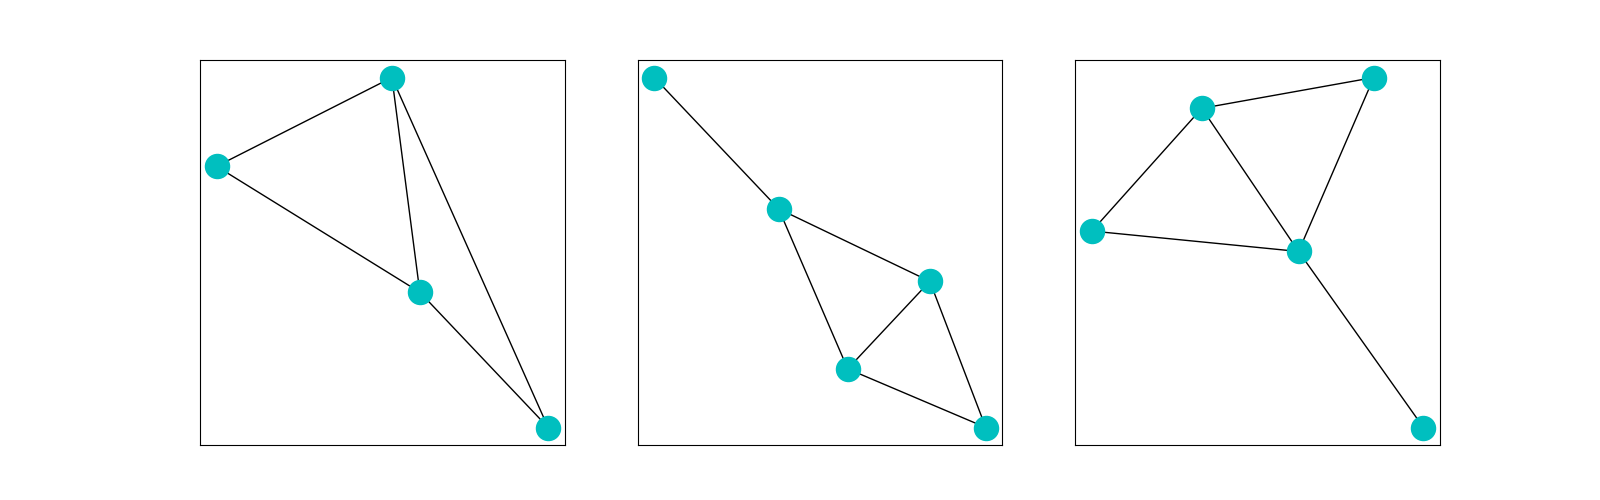
\includegraphics[width=10cm]{Images/H6_evolution.png}
    \centering
\end{figure}
\FloatBarrier

\begin{table}
    \centering
    \begin{tabular}{||c c c c||} 
    \hline
    Motif Count & Original Motif & Event 1 & Event 2\\ [0.5ex] 
    \hline\hline
    H3 & 2 & 4 & 4\\ 
    \hline
    H4 & 1 & 2 & 1\\
    \hline
    H5 & 1 & 2 & 1\\
    \hline
    H6 & 1 & 2 & 1\\
    \hline
    H7 & 1 & 2 & 1\\
    \hline
    H8 & 1 & 2 & 1\\
    \hline
   \end{tabular}
   \caption{Variations of the $T2$ event on the $H6$ motif}
    \label{table:4}
\end{table}

\section{H7}
$H7$ motifs feature prominently given certain parameters in the Thij model. This is another consequece
of $S_k$ induced subgraphs in the networks. Connecting any two of the outer edges of $S_k$
will generate ${k-2 \choose 2}$ $H7$ motifs. Generally those outer edges will connect, certainly 
in the preferential attachment model for $m=2$ and certainly in the Thij model as a consenquence 
of the $T3$ event.

\begin{figure}[!ht]
    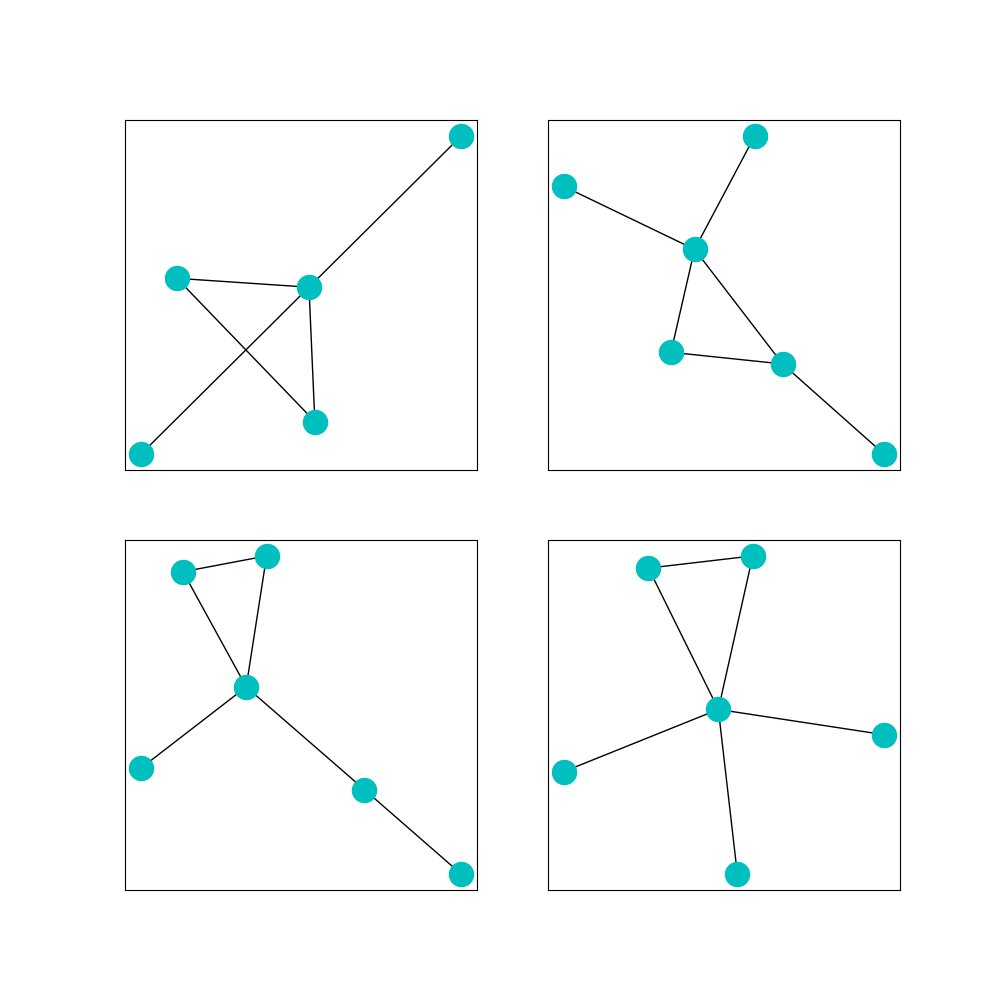
\includegraphics[width=8cm]{Images/H7_evolution.png}
    \centering
\end{figure}
\FloatBarrier

\begin{table}
    \centering
    \begin{tabular}{||c c c c c||} 
    \hline
    Motif Count & Original Motif & Event 1 & Event 2 & Event 3 \\ [0.5ex] 
    \hline\hline
    H3 & 2 & 3 & 5 & 5\\ 
    \hline
    H4 & 2 & 3 & 2 & 5 \\
    \hline
    H5 & 2 & 2 & 1 & 4 \\
    \hline
    H6 & 0 & 0 & 0 & 0 \\
    \hline
    H7 & 1 & 2 & 1 & 3 \\
    \hline
    H8 & 0 & 2 & 0 & 0\\
    \hline
   \end{tabular}
   \caption{Variations of the $T2$ event on the $H7$ motif}
   \label{table:5}
\end{table}

\section{H8}
The $H8$ motif is another we expect to appear fairly often. The $H8$
is two $H4$'s that share an edge and and a node. The $H8$ motif 
relies on connects at the center to form an induced $C3$ subgraph, but after an 
edge is added to one of the vertices of the induced $C3$ subgraph the 
$H8$ count would increase by the sum of edges attached to any of the other vertices. 

\begin{figure}[!ht]
    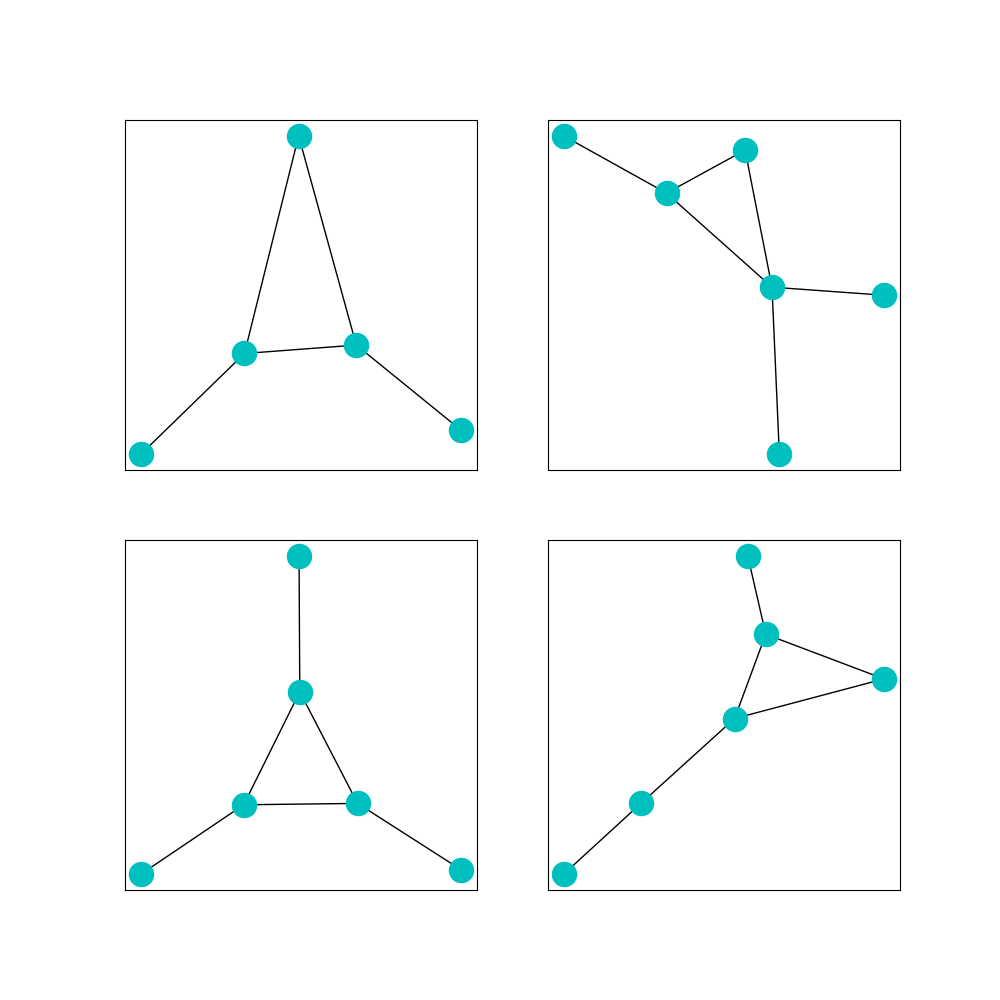
\includegraphics[width=8cm]{Images/H8_evolution.png}
    \centering
\end{figure}

\FloatBarrier
\begin{table}
    \centering
    \begin{tabular}{||c c c c c||} 
    \hline
    Motif Count & Original Motif & Event 1 & Event 2 & Event 3 \\ [0.5ex] 
    \hline\hline
    H3 & 2 & 3 & 5 & 5\\ 
    \hline
    H4 & 2 & 3 & 2 & 5 \\
    \hline
    H5 & 2 & 2 & 1 & 4 \\
    \hline
    H6 & 0 & 0 & 0 & 0 \\
    \hline
    H7 & 1 & 2 & 1 & 3 \\
    \hline
    H8 & 0 & 2 & 0 & 0\\
    \hline
   \end{tabular}
   \caption{Variations of the $T2$ event on the $H8$ motif}
   \label{table:6}
\end{table}

\section{H9}
The $H9$ motifs do not form around stars in the same way we might expect $H7$ and $H8$ to 
do so. In fact examining the manner in which the motifs above form new motifs given an event,
we see no $H9$'s generated. Genertaing $H9$'s would demand atleast edges between a new node and two 
different existing nodes or an event which producecs an edge between two existing nodes. We might expect
some $H9$'s to appear throughtout a network, but not necessarily be one of the dominating motif counts.

\begin{figure}[!ht]
    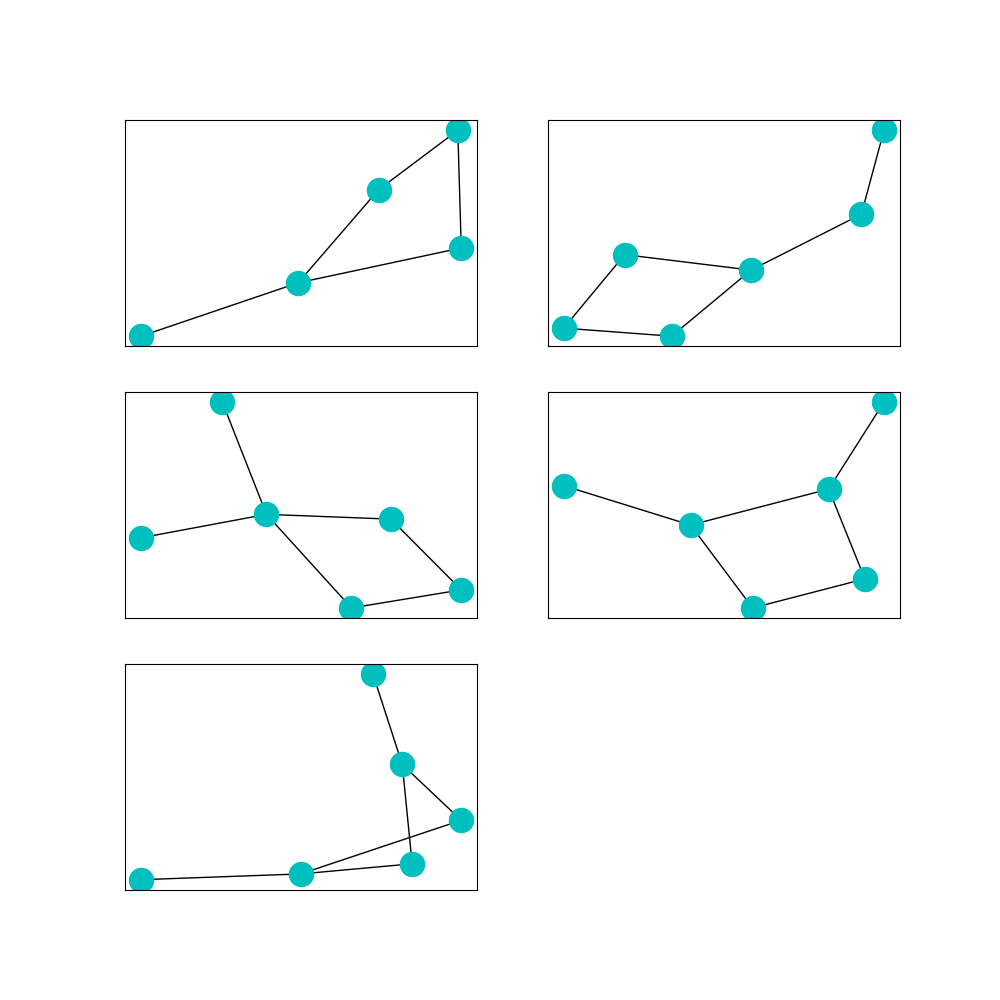
\includegraphics[width=8cm]{Images/H9_evolution.png}
    \centering
\end{figure}

\begin{table}
    \centering
    \begin{tabular}{||c c c c c c ||} 
    \hline
    Motif Count & Original Motif & Event 1 & Event 2 & Event 3  & Event 4\\ [0.5ex] 
    \hline\hline
    H3 & 6 & 8 & 8 & 9 & 8\\ 
    \hline
    H4 & 1 & 1 & 4 & 2 & 2 \\
    \hline
    H5 & 0 & 0 & 0 & 0 & 0\\
    \hline
    H6 & 0 & 0 & 0 & 0 & 0\\
    \hline
    H7 & 0 & 0 & 0 & 0 & 0\\
    \hline
    H8 & 0 & 0 & 0 & 0& 0\\
    \hline
    H9 & 1 & 1 & 2 & 2 &2\\
    \hline
   \end{tabular}
   \caption{Variations of the $T2$ event on the $H9$ motif}
   \label{table:7}
\end{table}

\section{H10}
The $H10$ is simply the $H9$ with an extra vertex and an edge between that vertex and the 
single vertex of degree one, which is attached to a single vertex on the edge of the simple
four walk $C4$ induced subgraph. Many $H10$'s could be generated from a single $H9$ if many vertices
attach to the single vertex of degree one in the $H9$ motif. We would a see a star graph From
with that vertex at the center. This may require an $H9$ already present as the induced star subgraph
would grow rapidly by the preferential mechanism and the probablity of an $H10$ would then decrease over
time.

\begin{figure}[!ht]
    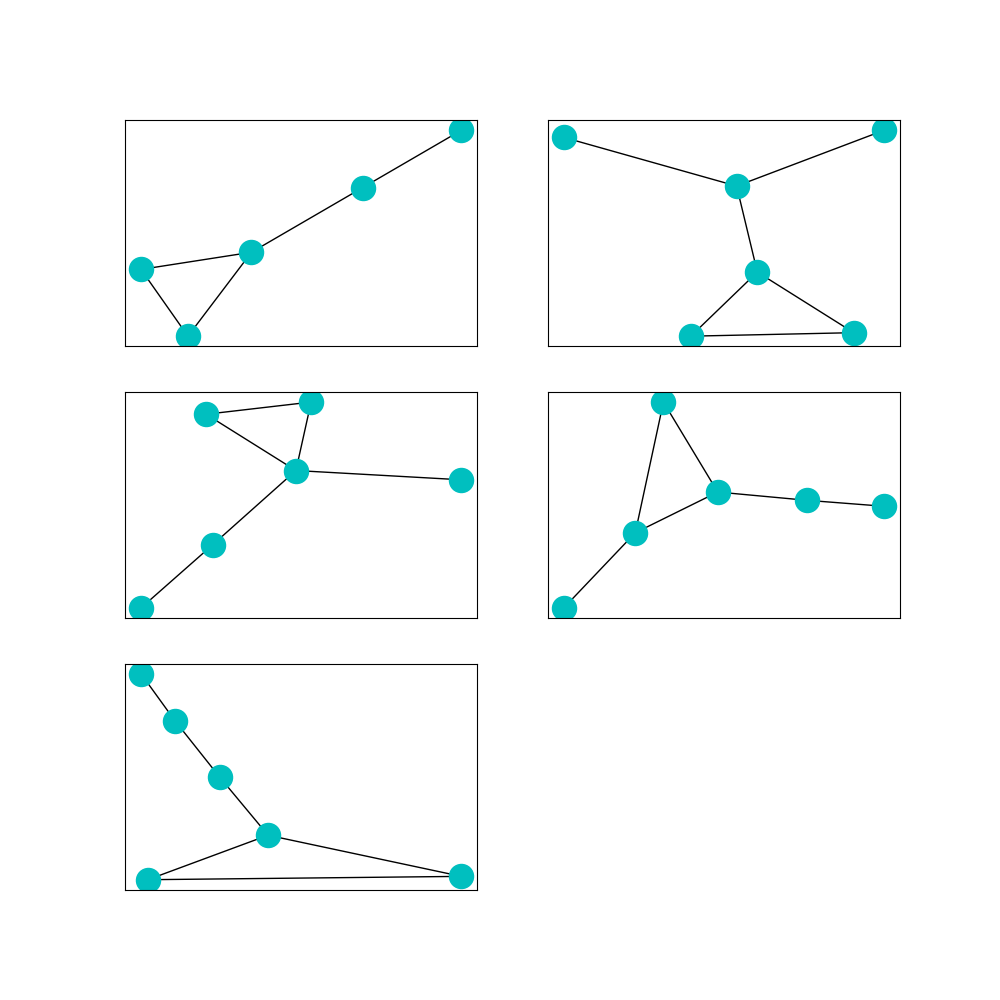
\includegraphics[width=8cm]{Images/H10_evolution.png}
    \centering
\end{figure}

\begin{table}
    \centering
    \begin{tabular}{||c c c c c c ||} 
    \hline
    Motif Count & Original Motif & Event 1 & Event 2 & Event 3  & Event 4 \\ [0.5ex] 
    \hline\hline
    H3 & 4 & 6 & 7 & 7  & 5\\
    \hline
    H4 & 1 & 2 & 4 & 2  & 1\\
    \hline
    H5 & 1 & 1 & 2 & 2 & 1\\
    \hline
    H6 & 0 & 0 & 0 & 0  & 5\\
    \hline
    H7 & 0 & 0 & 1 & 0 & 0 \\
    \hline
    H8 & 0 & 0 & 0 & 1 & 0 \\
    \hline
    H9 & 0 & 0 & 0 & 0  & 0 \\
    \hline
    H10 & 1 & 2 & 1 & 1 & 1 \\
    \hline
   \end{tabular}
   \caption{Variations of the $T2$ event on the $H10$ motif}
   \label{table:8}
\end{table}

\FloatBarrier

\section{H11}
The $H11$ motif, shaped like a bow-tie, is formed by the two three walks, triangles, that share a common
vertices. The formation of this motif does need $m \geq 2$ in the Barabási–Albert model or 
the possibility of a $T3$ event to form an edge between two existing nodes. 

\begin{figure}[!ht]
    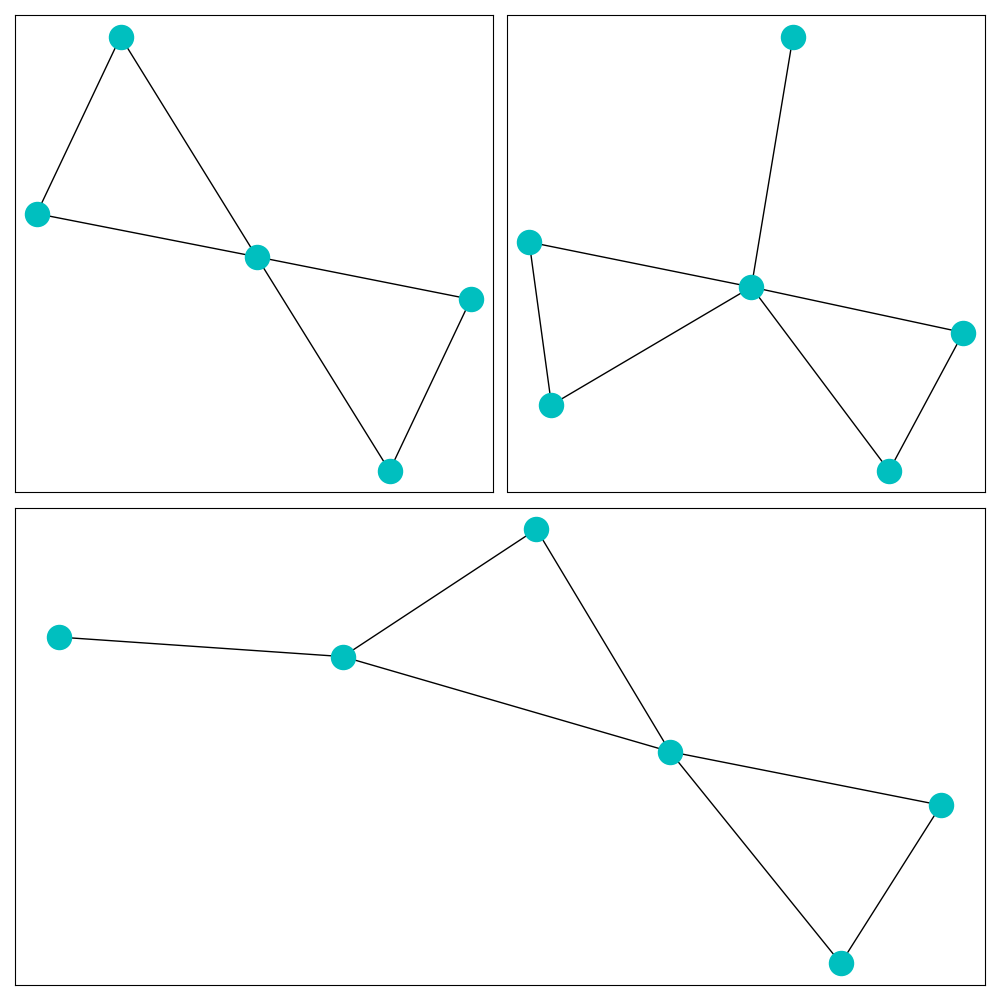
\includegraphics[width=8cm]{Images/H11_evolution.png}
    \centering
\end{figure}

\begin{table}
    \centering
    \begin{tabular}{||c c c c||} 
    \hline
    Motif Count & Original Motif & Event 1 & Event 2 \\ [0.5ex] 
    \hline\hline
    H3 & 8 & 12 & 12 \\ 
    \hline
    H4 & 4 & 5 & 10  \\
    \hline
    H5 & 0 & 5 & 6  \\
    \hline
    H6 & 0 & 0 & 0  \\
    \hline
    H7 & 2 & 2 & 6 \\
    \hline
    H8 & 0 & 2 & 0 \\
    \hline
    H9 & 0 & 0 & 0 \\
    \hline
    H10 & 4 & 5 & 4 \\
    \hline
    H11 & 1 & 1 & 1\\
    \hline
   \end{tabular}
   \caption{Variations of the $T2$ event on the $H11$ motif}
   \label{table:9}
\end{table}

\FloatBarrier

\section{H12}
$H12$, shaped like a house, contains five nodes, six edges, with an induced simple four-walk subgraph
and a single vertex attached to two vertices they themselves connected. The $H12$ like other
motifs containing an induced simple four-walk is not a-priori expected to have a relatively large count
given the preferetial attachment mechanism. 

\begin{figure}[!ht]
    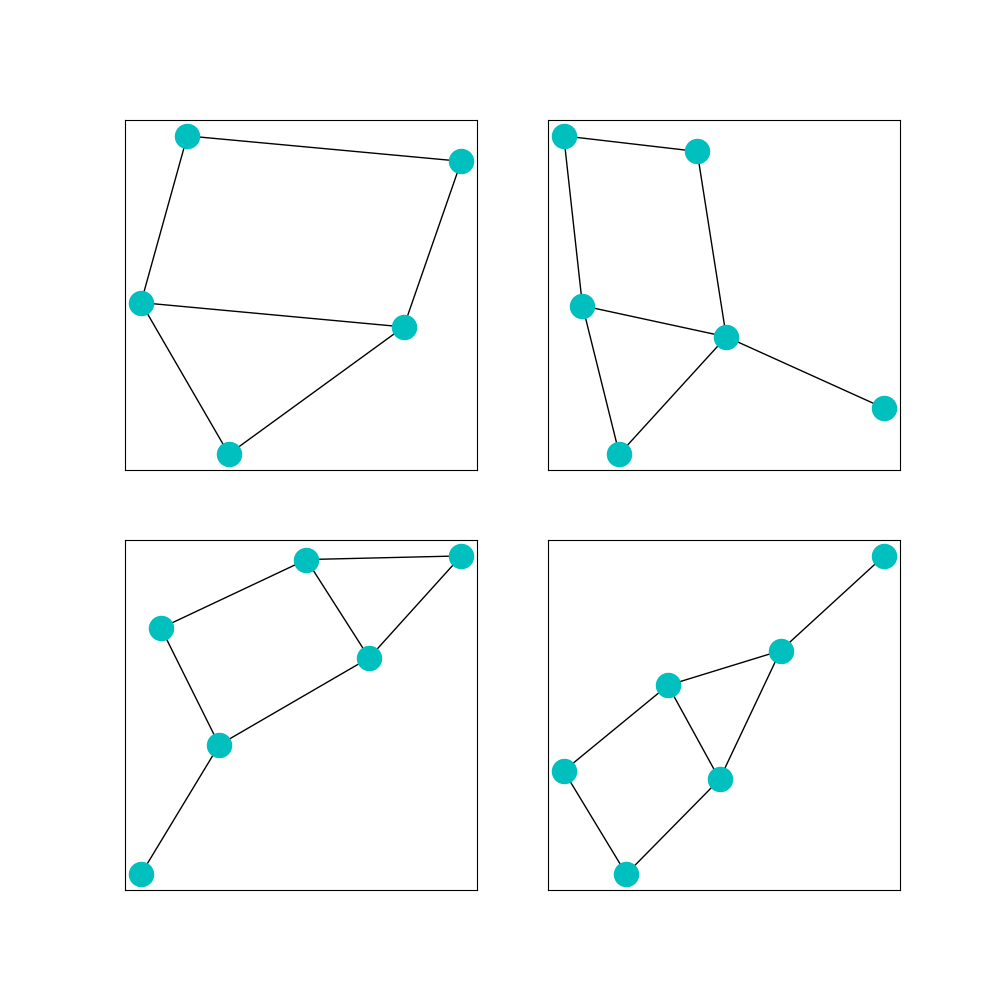
\includegraphics[width=8cm]{Images/H12_evolution.png}
    \centering
\end{figure}

\begin{table}
    \centering
    \begin{tabular}{||c c c c c||} 
    \hline
    Motif Count & Original Motif & Event 1 & Event 2 & Event 3 \\ [0.5ex] 
    \hline\hline
    H3 & 10 & 14 & 13 & 14\\ 
    \hline
    H4 & 2 & 5 & 3 & 3 \\
    \hline
    H5 & 2 & 3 & 2 & 3 \\
    \hline
    H6 & 0 & 0 & 0 & 0 \\
    \hline
    H7 & 0 & 1 & 0 & 0 \\
    \hline
    H8 & 1 & 2 & 1 & 3\\
    \hline
    H9 & 2 & 3 & 3 & 2 \\
    \hline
    H10 & 2 & 2 & 3 & 2 \\
    \hline
    H11 & 0 & 0 & 0 & 0 \\
    \hline
    H12 & 1 & 1 & 1 & 1\\
    \hline
   \end{tabular}
   \caption{Variations of the $T2$ event on the $H12$ motif}
   \label{table:10}
\end{table}


\FloatBarrier

\section{H13}
Finally we come to the $H13$. The $H13$ could plausibly form in the $m \geq 2$ case for the 
Barabási–Albert model, but it would require new node being consistently attached to the 
same two nodes repeatedly. There would also need to be an existing connection between those two nodes
that are being attached to. Thus for the Barabási–Albert graph the presence of an H13 is sensitive
to the initial graph and it's early development when there might still be a 'more uniform' probability
of attachment.

\begin{figure}[!ht]
    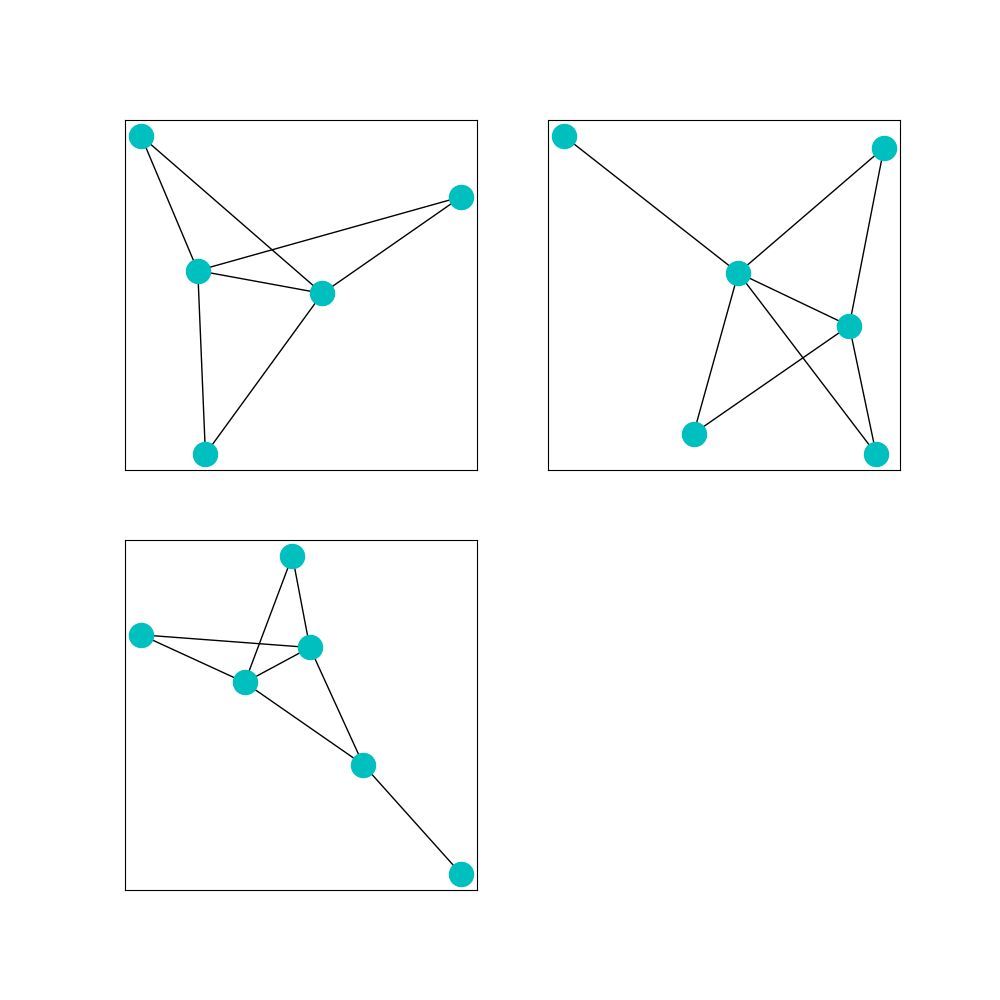
\includegraphics[width=8cm]{Images/H13_evolution.png}
    \centering
    \caption{The H13 Graph and possible node attachments up to symmetry.}
\end{figure}

\begin{table}
    \centering
    \begin{tabular}{||c c c c||} 
    \hline
    Motif Count & Original Motif & Event 1 & Event 2 \\ [0.5ex] 
    \hline\hline
    H3 & 18 & 24 & 24\\ 
    \hline
    H4 & 8 & 14 & 9  \\
    \hline
    H5 & 12 & 15 & 13  \\
    \hline
    H6 & 3 & 3 &3  \\
    \hline
    H7 & 6 & 12 & 6 \\
    \hline
    H8 & 6 & 12 & 10\\
    \hline
    H9 & 6 & 9 & 8 \\
    \hline
    H10 & 0 & 0 & 4  \\
    \hline
    H11 & 0 & 0 & 0  \\
    \hline
    H12 & 0 & 0 & 0 \\
    \hline
    H13 & 1 & 1 & 1 \\
    \hline
   \end{tabular}
   \caption{Variations of the $T2$ event on the $H13$ motif}
   \label{table:11}
\end{table}

\section{In Summary of T2 events}

If we consider the manner in which preferential attachment develops we begin with a cluster of uniformly
connected nodes and proceed to add nodes and edges with the edges between the new node and some existing node.
As these new edges are more likely to attach to those nodes that already have a large number
of edges attached we can easily imagine an overlay of $H4$'s very quickly forming. However in the 
preferential attachment model we also specify how many $m$ nodes the new nodes attaches to. Thus it's most probable
that the preferential attachmnent model connects to the node that's already most connected 
and some other node who may or may not be heavily connected. Here with $m \geq 2$ triangles may more 
commonly form thus generating $H5$'s, $H7$'s , or $H8$'s.

\chapter{Twitter Model Specific Motif Evolution}

Given that we allow our network to evolve over time new additions of edges or nodes will cause changes
in the total number of appearances of the present motifs. Which new motifs appear is consequent of
which motifs are already present and how a new node or edge is added. Above we specified three possible
events a new root node, a new node and edge, or a new edge between existing nodes 
($T1$, $T2$, $T3$ respectively). When we consider the Twitter model we need only consider the 
case in which an edge is added between existing nodes as the case in which a new node is added is already
considered above in our preferential attachment case. There may be different probabilities associated with the 
above attachment, but we will make some preliminary speculation about how the dynamics might be different overall.

The $T3$ event chooses attachment based on the superstar mechanism. Thij found $q=0.9$ to be the best 
probability for the superstar mechanism to generate temporal development in the network
most similar to observed Twitter behavior. \cite{thij} 

\section{H3}
xxxxx
\begin{figure}[!ht]
    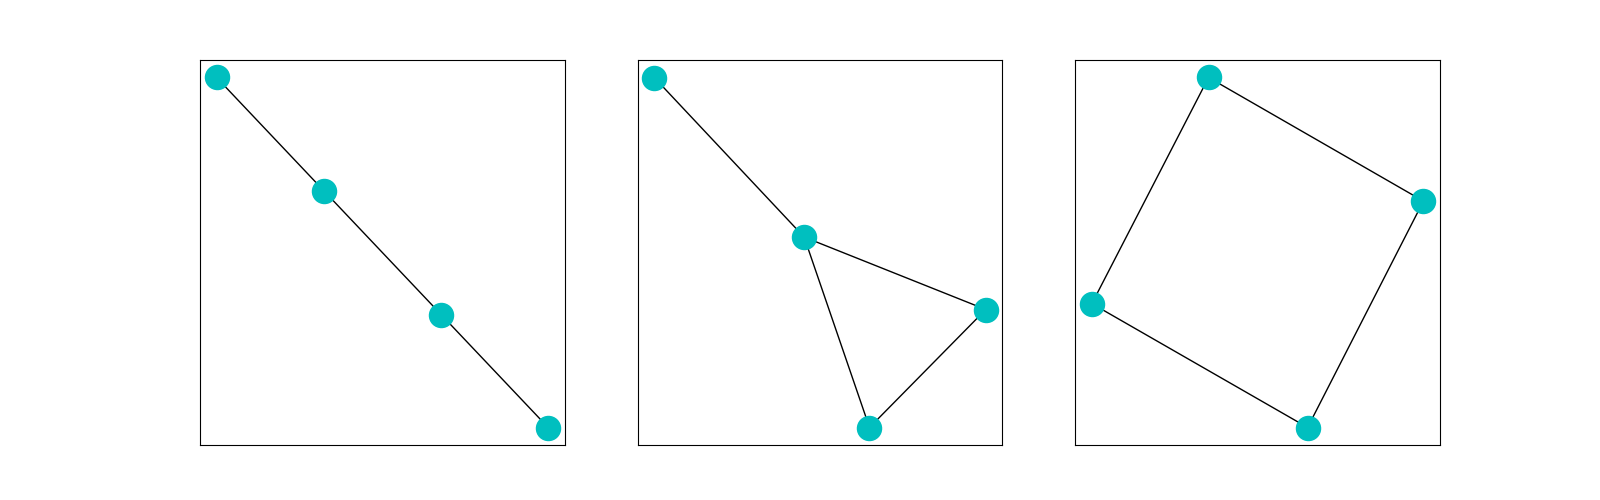
\includegraphics[width=8cm]{Images/H3_T3_evolution.png}
    \centering
\end{figure}

\begin{table}
    \centering
    \begin{tabular}{||c c c c||} 
    \hline
    Motif Count & Original Motif & Event 1 & Event 2\\ [0.5ex] 
    \hline\hline
    H3 & 1 & 2 & 4\\ 
    \hline
    H4 & 0& 1 & 0  \\
    \hline
    H5 & 0& 1 & 0  \\
    \hline
   \end{tabular}
   \caption{Variations of the $T3$ event on the $H2$ motif}
   \label{table:12}
\end{table}

\section{H4}
Due to the three symmetry of $H4$ adding an edge between any two unconnected nodes results in 
the formation of a single $H5$.

\begin{figure}[!ht]
    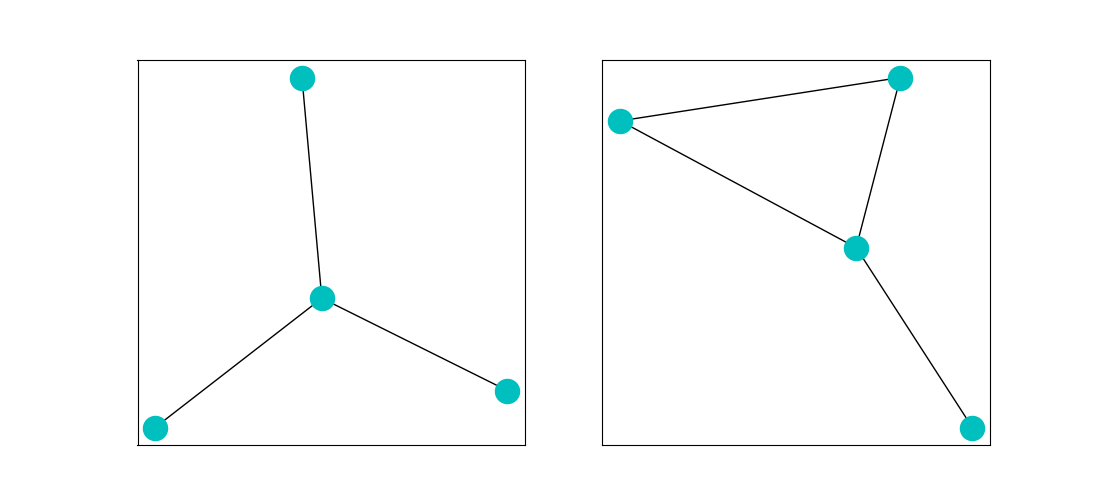
\includegraphics[width=8cm]{Images/H4_T3_evolution.png}
    \centering
\end{figure}

\begin{table}
    \centering
    \begin{tabular}{||c c c||} 
    \hline
    Motif Count & Original Motif & Event 1 \\ [0.5ex] 
    \hline
    H3 & 0 & 2 \\ 
    \hline
    H4 & 1 & 1 \\
    \hline
    H5 & 0 & 1 \\
    \hline
   \end{tabular}
   \caption{Variations of the $T3$ event on the $H13$ motif}
   \label{table:13}
\end{table}

\section{H5}
Here we have two symmetry and so connecting any two unconnected edges of the $H5$ produces an $H6$.

\begin{figure}[!ht]
    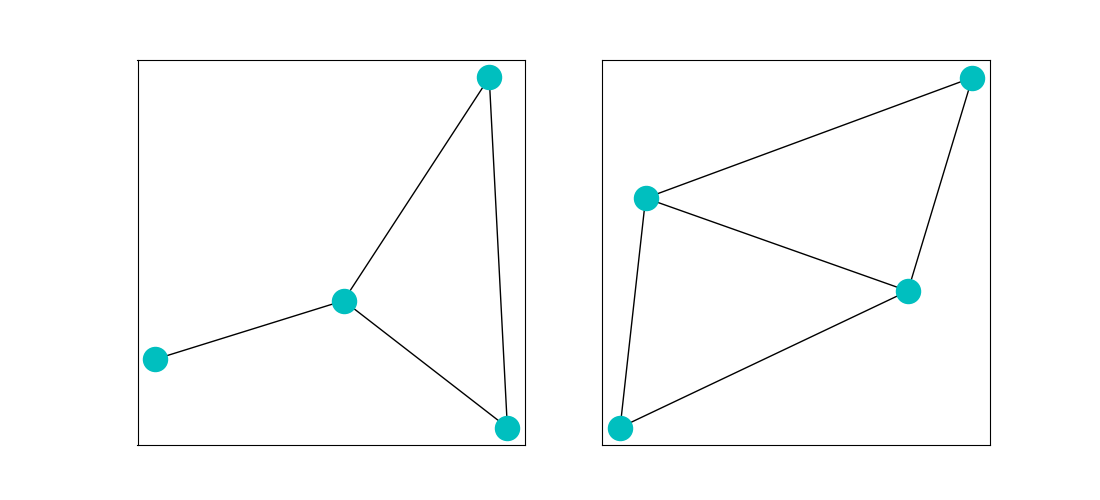
\includegraphics[width=8cm]{Images/H5_T3_evolution.png}
    \centering
\end{figure}

\begin{table}
    \centering
    \begin{tabular}{||c c c||} 
    \hline
    Motif Count & Original Motif & Event 1 \\ [0.5ex] 
    \hline\hline
    H3 & 2 & 6\\ 
    \hline
    H4 & 1 & 2 \\
    \hline
    H5 & 1 & 4\\
    \hline
    H6 & 0 & 1\\
    \hline
   \end{tabular}
   \caption{Variations of the $T3$ event on the $H13$ motif}
   \label{table:14}
\end{table}

\section{H6}
Adding an edge to $H6$ generates a complete graph of four nodes. 

\begin{figure}[!ht]
    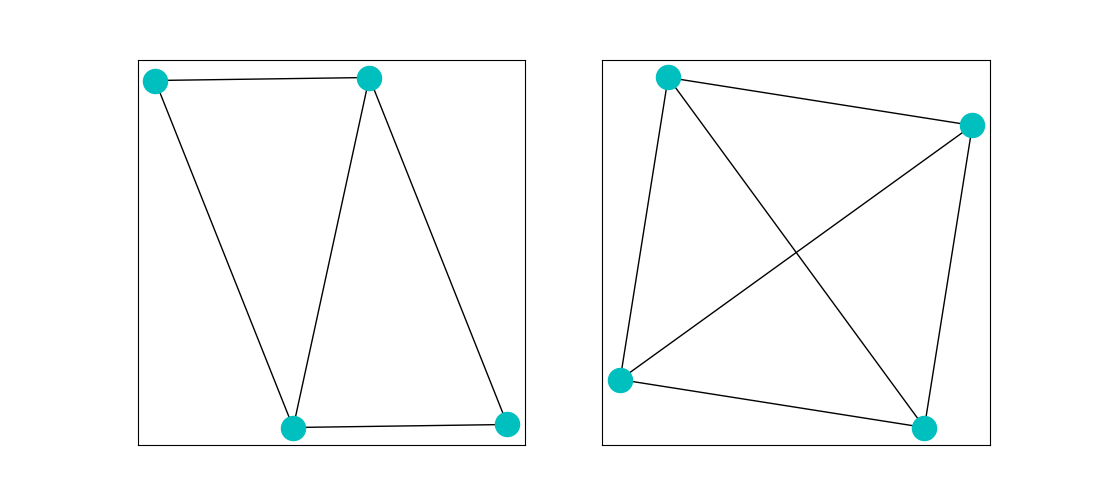
\includegraphics[width=8cm]{Images/H6_T3_evolution.png}
    \centering
\end{figure}

\begin{table}
    \centering
    \begin{tabular}{||c c c ||} 
    \hline
    Motif Count & Original Motif & Event 1  \\ [0.5ex] 
    \hline\hline
    H3 & 6 & 12 \\ 
    \hline
    H4 & 2 & 4 \\
    \hline
    H5 & 4 & 12 \\
    \hline
    H6 & 1 & 6 \\
    \hline
    \hline
   \end{tabular}
   \caption{Variations of the $T3$ event on the $H6$ motif}
   \label{table:15}
\end{table}

\section{H7}
Adding edges in the $H7$ motif gives to only two distinct graphs once again as 
a consequence of the motif's symmetry. 
 
\begin{figure}[!ht]
    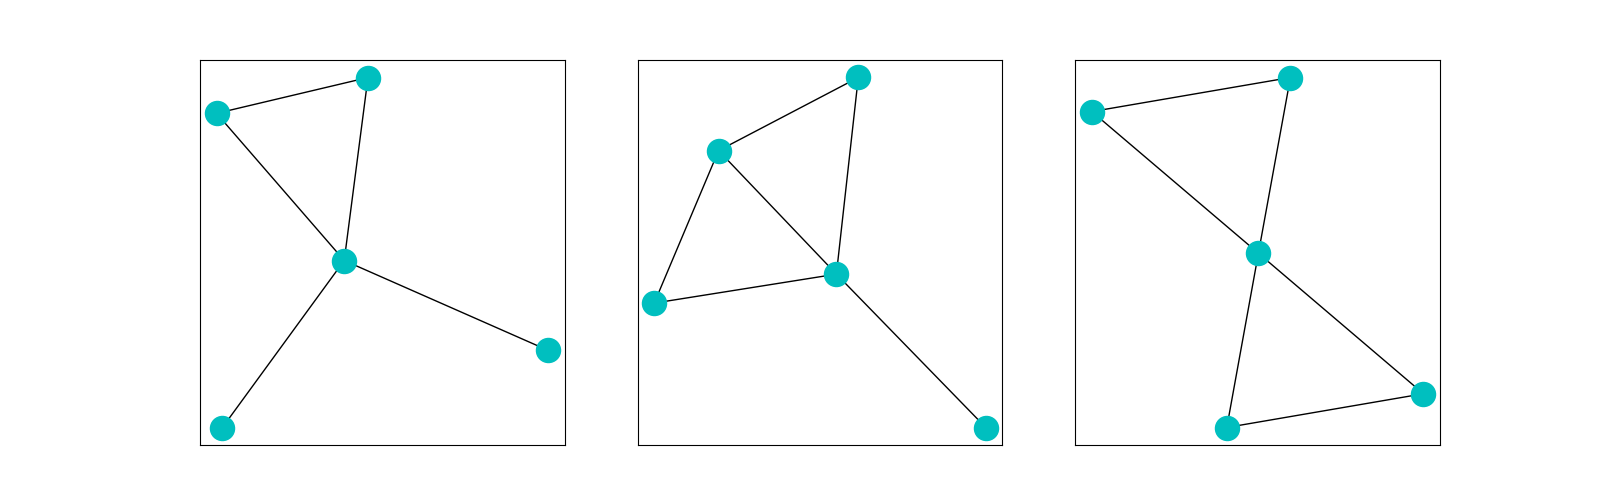
\includegraphics[width=12cm]{Images/H7_T3_evolution.png}
    \centering
\end{figure}

\begin{table}
    \centering
    \begin{tabular}{||c c c c c||} 
    \hline
    Motif Count & Original Motif & Event 1 & Event 2 & Event 3 \\ [0.5ex] 
    \hline\hline
    H3 & 2 & 3 & 5 & 5\\ 
    \hline
    H4 & 2 & 3 & 2 & 5 \\
    \hline
    H5 & 2 & 2 & 1 & 4 \\
    \hline
    H6 & 0 & 0 & 0 & 0 \\
    \hline
    H7 & 1 & 2 & 1 & 3 \\
    \hline
    H8 & 0 & 2 & 0 & 0\\
    \hline
   \end{tabular}
   \caption{Variations of the $T3$ event on the $H7$ motif}
   \label{table:16}
\end{table}

\section{H8}
The $H8$ motif here generates three different motifs depending upon the nodes which become connected.
\begin{figure}[!ht]
    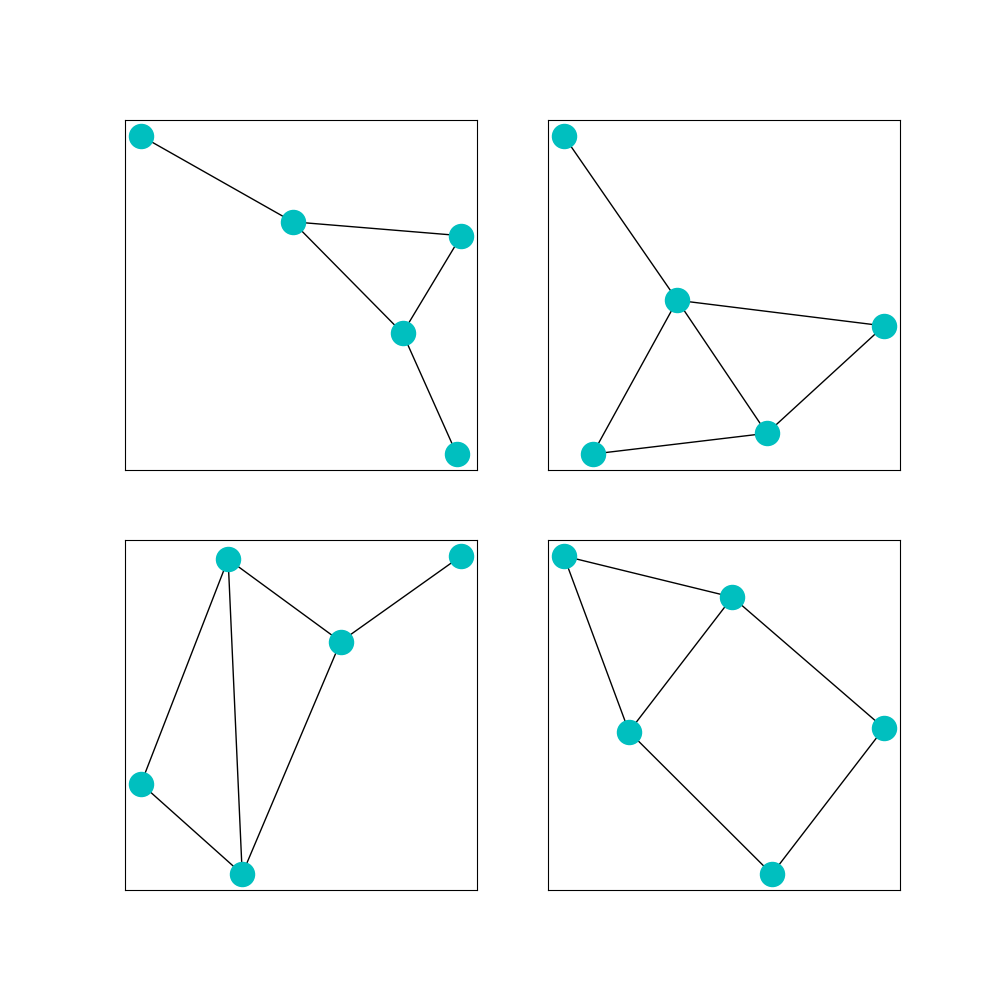
\includegraphics[width=8cm]{Images/H8_T3_evolution.png}
    \centering
\end{figure}

\begin{table}
    \centering
    \begin{tabular}{||c c c c c||} 
    \hline
    Motif Count & Original Motif & Event 1 & Event 2 & Event 3 \\ [0.5ex] 
    \hline\hline
    H3 & 5 & 10 & 10 & 10\\ 
    \hline
    H4 & 2 & 5 & 3 & 2 \\
    \hline
    H5 & 2 & 6 & 5 & 2 \\
    \hline
    H6 & 0 & 1 & 1 & 0 \\
    \hline
    H7 & 0 & 2 & 0 & 0 \\
    \hline
    H8 & 1 & 2 & 2 & 1\\
    \hline
    H9 & 0 & 1 & 1 & 2\\
    \hline
    H10  & 0 & 0 & 2& 2 \\
    \hline
    H11  & 0 & 0 & 1& 0 \\
    \hline
    H12  & 0 & 0 & 0& 0 \\
    \hline
   \end{tabular}
   \caption{Variations of the $T3$ event on the $H8$ motif}
   \label{table:17}
\end{table}

\section{H9}
An $H9$ motif with an edge added anywhere doesn't produce a combinatorial jump the sample
way other motifs might. An appearance of the $H9$ motif already
requires a certain amount of local connectivity.

\begin{figure}
    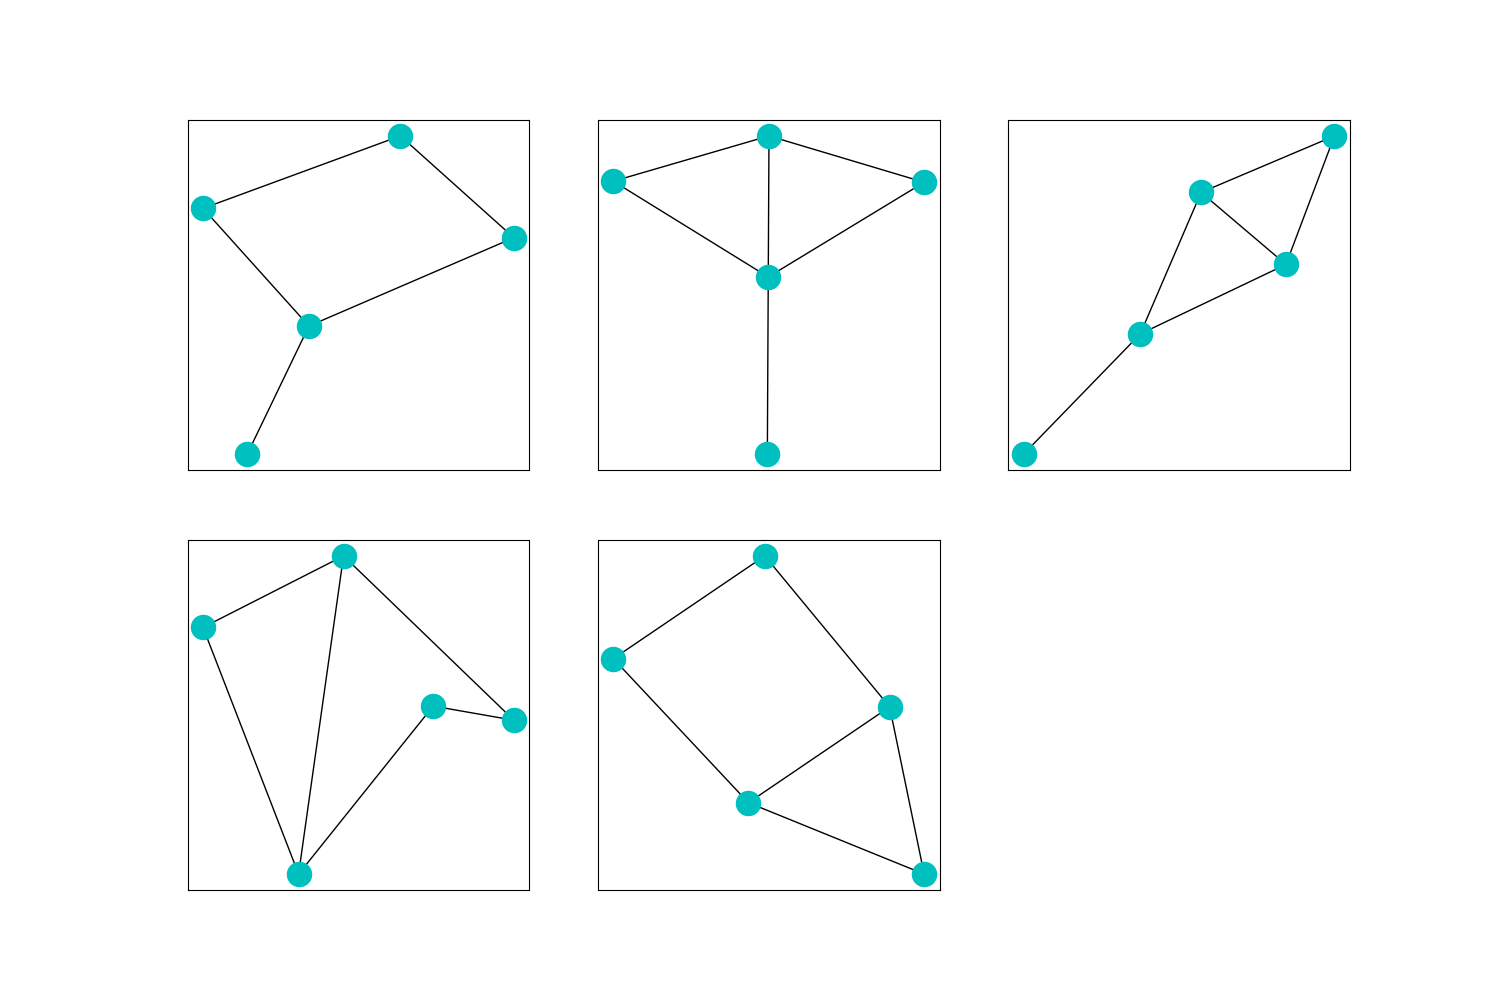
\includegraphics[width=12cm]{Images/H9_T3_evolution.png}
    \centering
    
\end{figure}

\begin{table}
    \centering
    \begin{tabular}{||c c c c c c||} 
    \hline
    Motif Count & Original Motif & Event 1 & Event 2 & Event 3 & Event 4 \\ [0.5ex] 
    \hline\hline
    H3 & 6 & 10 & 10 & 10 & 10\\ 
    \hline
    H4 & 1 & 5 & 3 & 2 & 2 \\
    \hline
    H5 & 0 & 6 & 5 & 2 & 2 \\
    \hline
    H6 & 0 & 1 & 1 & 0 & 0 \\
    \hline
    H7 & 1 & 2 & 1 & 0 & 0 \\
    \hline
    H8 & 0 & 2 & 2 & 1 & 1\\
    \hline
    H9 & 1 & 1 & 2 & 2 & 2\\
    \hline
    H10 & 0 & 0 & 2 & 2 & 2\\
    \hline
    H11 & 0 & 0 & 0 & 0 & 0\\
    \hline
    H12 & 0 & 0 & 0 & 1 & 1\\
    \hline
   \end{tabular}
   \caption{Variations of the $T3$ event on the $H9$ motif}
   \label{table:18}
\end{table}

\section{H10}
The $H10$ motif is

\begin{figure}
    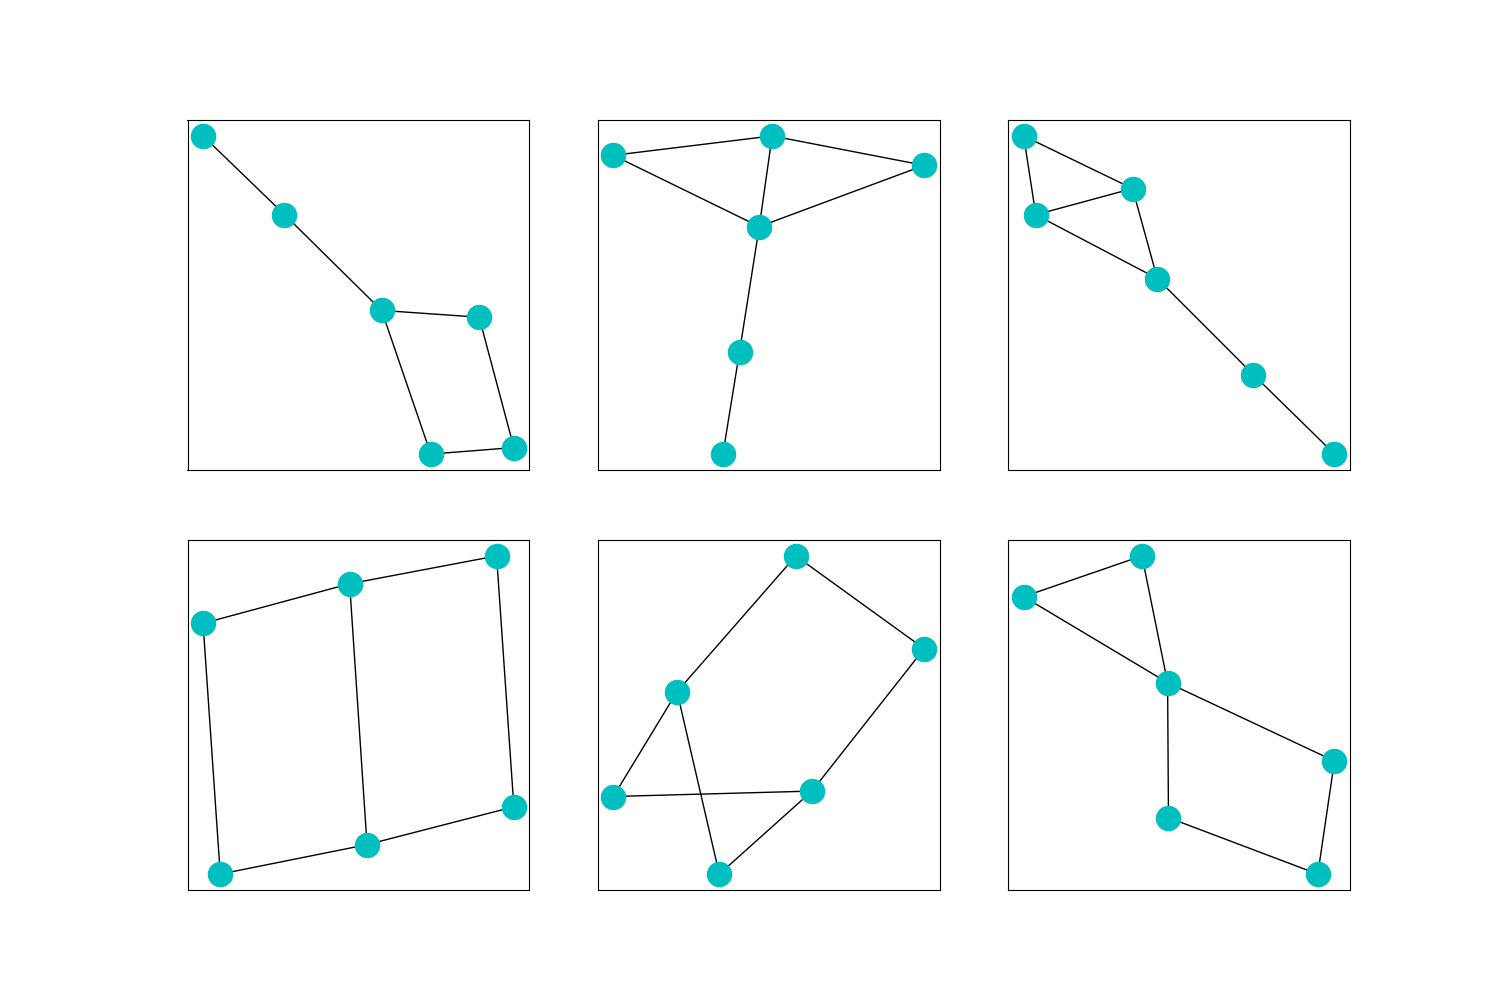
\includegraphics[width=15cm]{Images/H10_T3_evolution.png}
\end{figure}
\begin{table}
    \centering
    \begin{tabular}{||c c c c c||} 
    \hline
    Motif Count & Original Motif & Event 1 & Event 2 & Event 3 \\ [0.5ex] 
    \hline\hline
    H3 & 4 & 10 & 8 & 10 \\ 
    \hline
    H4 & 1 & 2 & 4 & 3 \\
    \hline
    H5 & 1 & 2 & 4 & 5\\
    \hline
    H6 & 0 & 0 & 0 & 1 \\
    \hline
    H7 & 0 & 0 & 2 & 0 \\
    \hline
    H8 & 0 & 1 & 0 & 2\\
    \hline
    H9 & 0 & 2 & 0 & 1\\
    \hline
    H10 & 1 & 2 & 4 & 2\\
    \hline
    H11 & 0 & 0 & 1 & 0\\
    \hline
    H12 & 0 & 1 & 0 & 0\\
    \hline
   \end{tabular}
   \caption{Variations of the $T3$ event on the $H10$ motif}
   \label{table:19}
\end{table}

\section{H11}
xxxxx

\begin{figure}
    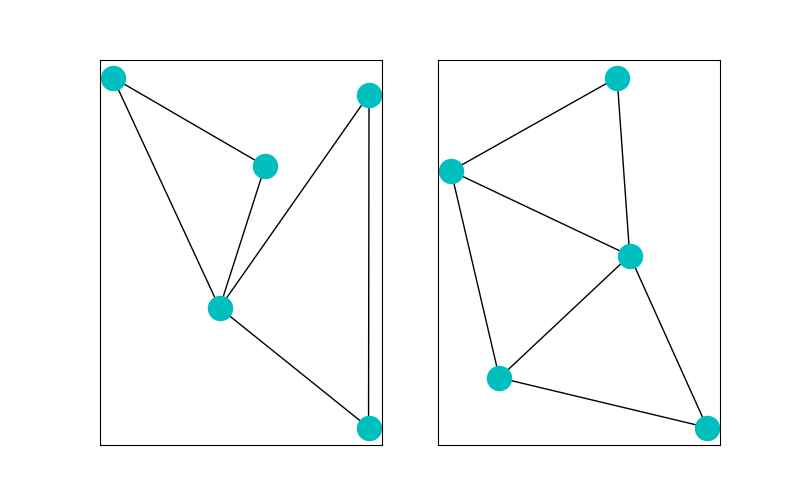
\includegraphics[width=10cm]{Images/H11_T3_evolution.png}
    \centering
\end{figure}

\begin{table}
    \centering
    \begin{tabular}{||c c c ||} 
    \hline
    Motif Count & Original Motif & Event 1 \\ [0.5ex] 
    \hline\hline
    H3 & 8 & 17 \\ 
    \hline
    H4 & 4 & 6  \\
    \hline
    H5 & 4 & 10 \\
    \hline
    H6 & 0 & 2 \\
    \hline
    H7 & 2 & 3 \\
    \hline
    H8 & 0 & 5 \\
    \hline
    H9 & 0 & 4 \\
    \hline
    H10 & 4 & 6 \\
    \hline
    H11 & 1 & 1 \\
    \hline
    H12 & 0 & 2 \\
    \hline
    H13 & 0 & 0 \\
    \hline
   \end{tabular}
   \caption{Variations of the $T3$ event on the $H11$ motif}
   \label{table:20}
\end{table}

\section{H12}
xxxxx

\begin{figure}
    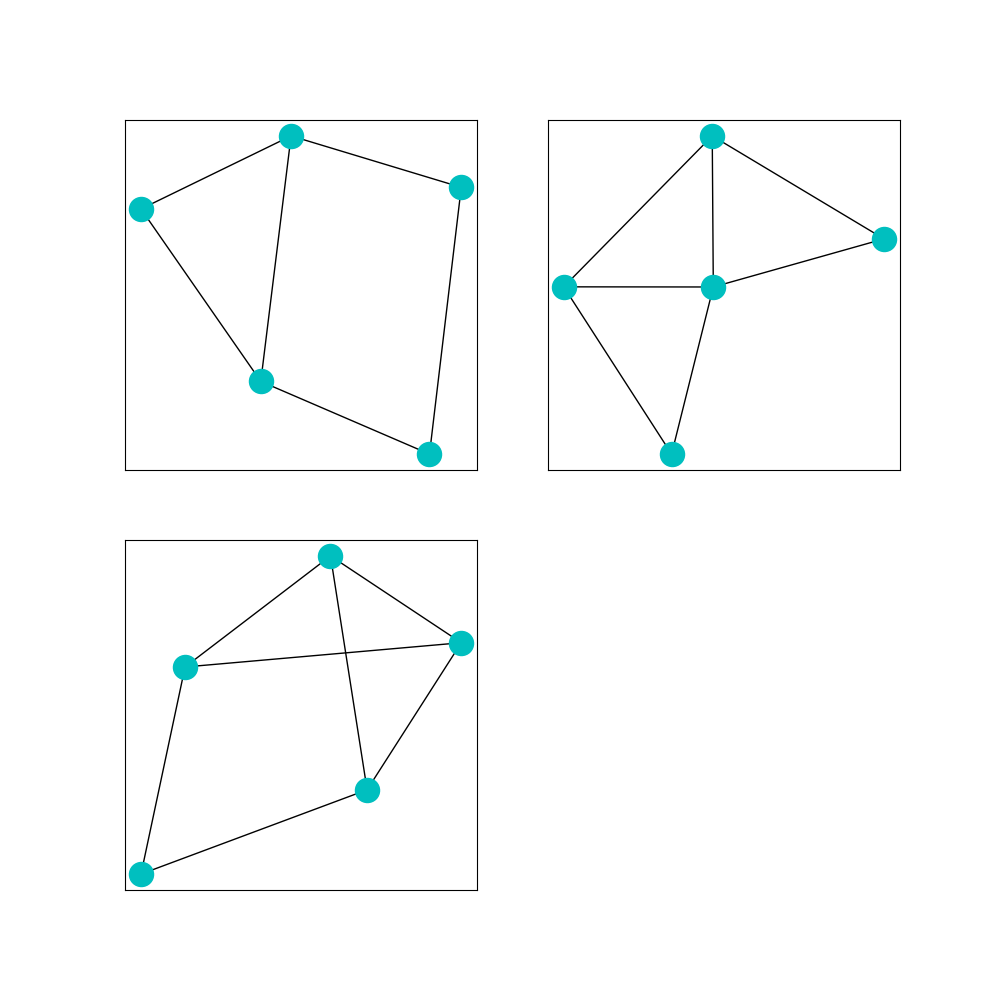
\includegraphics[width=10cm]{Images/H12_T3_evolution.png}
    \centering
\end{figure}

\begin{table}
    \centering
    \begin{tabular}{||c c c c||} 
    \hline
    Motif Count & Original Motif & Event 1 & Event 2\\ [0.5ex] 
    \hline\hline
    H3 & 10 & 17 & 18 \\ 
    \hline
    H4 & 2 & 6 & 4 \\
    \hline
    H5 & 2 & 10 & 6\\
    \hline
    H6 & 0 & 2 & 1 \\
    \hline
    H7 & 0 & 3 & 0\\
    \hline
    H8 & 1 & 5 & 4 \\
    \hline
    H9 & 2 & 4 & 8 \\
    \hline
    H10 & 2 & 6 & 6 \\
    \hline
    H11 & 0 & 1 & 0 \\
    \hline
    H12 & 1 & 2 & 4 \\
    \hline
    H13 & 0 & 0 & 0\\
    \hline
   \end{tabular}
   \caption{Variations of the $T3$ event on the $H12$ motif}
   \label{table:21}
\end{table}

\section{H13}
xxxxx
\begin{figure}
    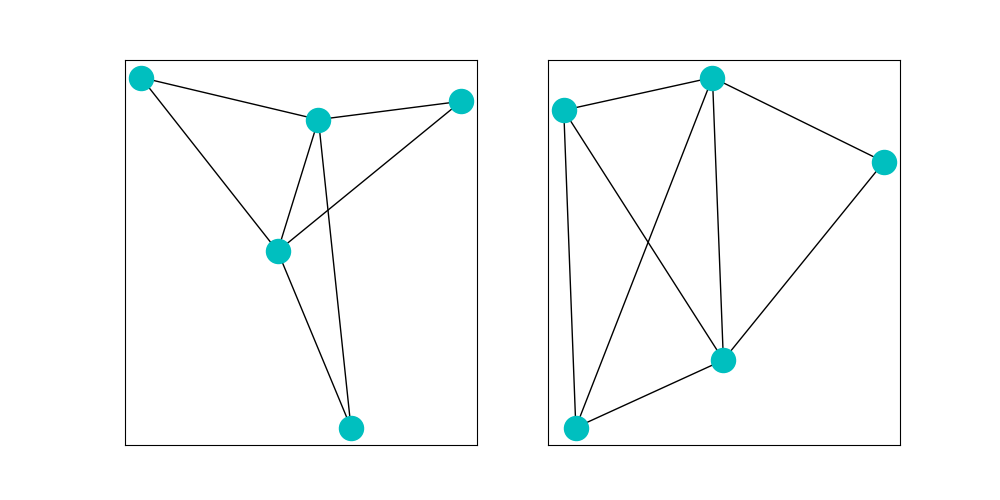
\includegraphics[width=10cm]{Images/H13_T3_evolution.png}
    \centering
\end{figure}

\begin{table}
    \centering
    \begin{tabular}{||c c c||} 
    \hline
    Motif Count & Original Motif & Event 1\\ [0.5ex] 
    \hline\hline
    H3 & 18 & 28 \\ 
    \hline
    H4 & 8 & 10 \\
    \hline
    H5 & 12 & 22 \\
    \hline
    H6 & 3 & 8 \\
    \hline
    H7 & 6 & 8 \\
    \hline
    H8 & 6 & 14 \\
    \hline
    H9 & 6 & 12 \\
    \hline
    H10 & 0 & 12 \\
    \hline
    H11 & 0 & 2 \\
    \hline
    H12 & 0 & 6 \\
    \hline
    H13 & 1 & 1\\
    \hline
   \end{tabular}
   \caption{Variations of the $T3$ event on the $H13$ motif}
   \label{table:22}
\end{table}


\section{In summary of the T3 events}

The $T3$ events above may explain some heavier clustering for high $\lambda$ in the Thij model allowing
for the generation of motifs that one may not see easily find using the induced star subgraph explanation. 
Adding in edges of existing nodes makes the likelihood of three-cycle or four-cycle subgraphs 
being found in the network.


\chapter{Motif Correlation}
As we've discussed we expect some motifs to correlate with others over time, but we 
can compute correlation and covariance matrices for the Barabási–Albert model and the Thij model
for a variety of parameters. There is order of magnitude difference in covariances between
motifs. Thus all covariance matrices are on a log scale.  If we begin with  a simulation of the Barabási–Albert model
we get the heat map below:


\begin{figure}
    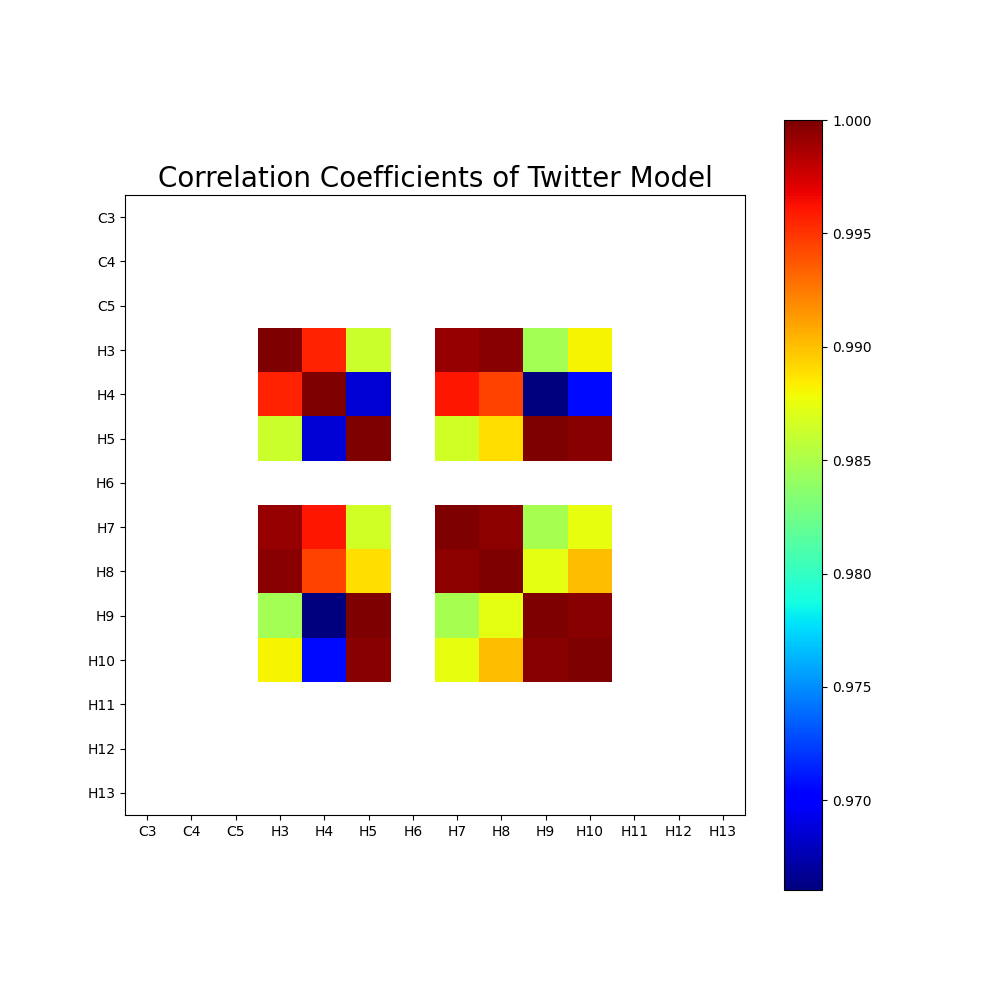
\includegraphics[width=8cm]{Images/CorrCoefPreferentialAttachmentModel.png}\
    \centering
    \caption{Barabási–Albert model with three initial nodes and $m=1$. We can see clearly that
    the model is capable of only producing certain motifs given the limitations of only 
    attaching a single edge and a single node at every time step. We also see that 
    H7's and H8's travel together. However appearances of those motifs depend upon the intialization
    of the graph itself.}
\end{figure}

\begin{figure}
    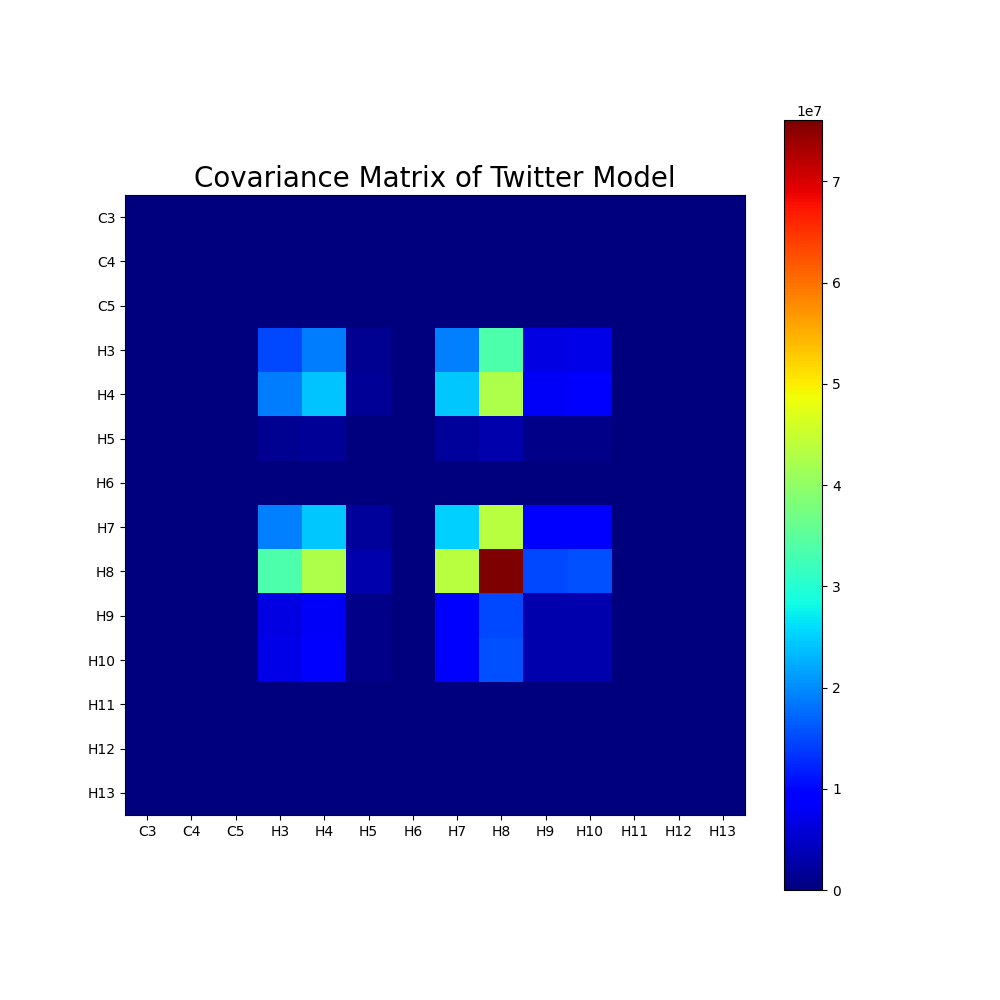
\includegraphics[width=08cm]{Images/CovMatPreferentialAttachmentModel.png}\
    \centering
    \caption{Barabási–Albert model with three initial nodes and $m=1$. Here we once again see that 
    the H7 and H8 motifs have a much higher covariance than any other pair of motifs.}
\end{figure}


The Barabási–Albert model is only capable of generating certain new motifs after the initilization if 
it can only add one edge at a time. Some motifs would require the introduction of an event
which can add edges between existing nodes. The only motifs that increase in size after this
sample of the Barabási–Albert model are $H2$,$H4$,$H5$,$H7$, $H8$, $H9$, and $H10$. There is a cluster
of nodes at the center and the new nodes introduced are gradually attracted to one node via the 
preferential attachment mechanism. However we will see that we can generate all motifs provided
$n>2$.


\begin{figure}
    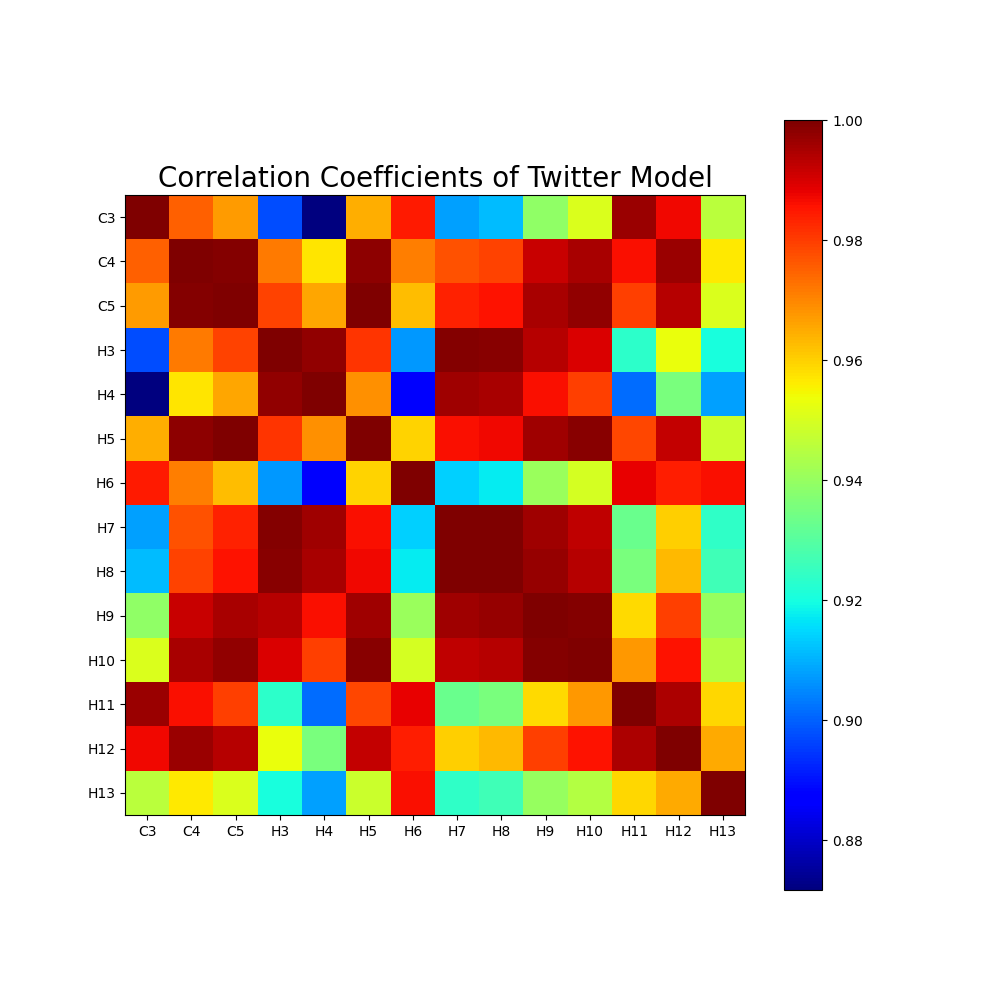
\includegraphics[width=8cm]{Images/CorrCoefPreferentialAttachmentModel2.png}\
    \centering
    \caption{Barabási–Albert model with three initial nodes and $m=2$. Here we see that all motifs 
    are present. They all have fairly high correlation coeffecients, but we see that the H7's and
    H8's are highly correlated as is H7 and H8 with H3.}
\end{figure}

\begin{figure}
    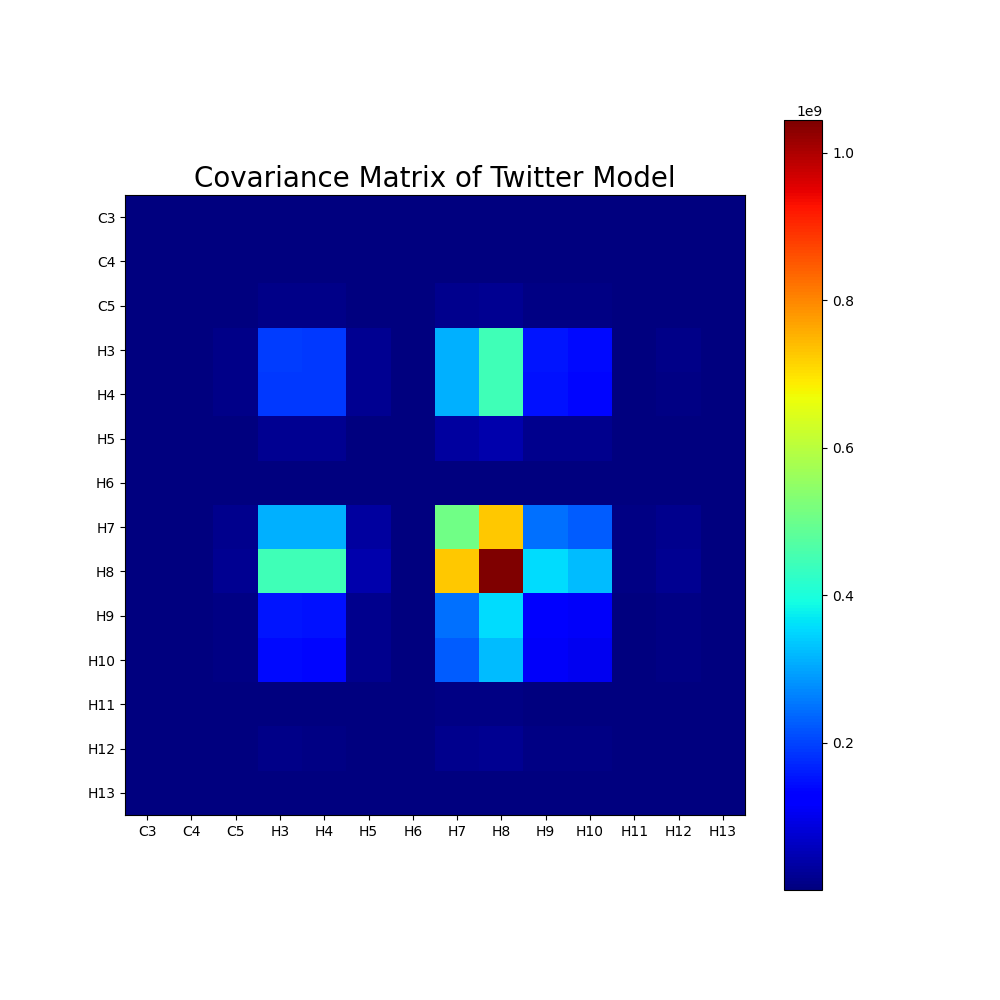
\includegraphics[width=08cm]{Images/CovMatPreferentialAttachmentModel2.png}\
    \centering
    \caption{Barabási–Albert model with three initial nodes and $m=2$. The covariance
    offers a different perspective than the correlation figure above. We now see that 
    there high covariancec between H7's and H8's, and we once again see a relationship
    between H8,H7,H3,H4, but many other motifs have a much,much smaller covariances.}
\end{figure}

Below we now have a Barabási–Albert simulation that resembles our Thij model for certain parameters. We 
see above that all motifs are generated over time now that the new node can attach to two existing nodes
rather than one. This allows for the formation of $C_3$ and $C_4$ subgraphs that are necessary for the
the motifs that also have $C_3$ and $c_4$ subgraphs. We also see that some of our a-priori speculation
above is supported by the correlation and covariance matrices. 


We recall that for relatively high $p$ we are more likely to attach a new node and a new
edge. For relatively low $p$ we attach a new edge between existing nodes. For relatively
high $\lambda$ we are likely to introduce a new message node without any attachments. 
Above we discussed that for higih $p$ we introde a new node and attach it with
a the superstar mechanism after selecting a message subgraph with the preferential
attachment mechanism.

\begin{figure}
    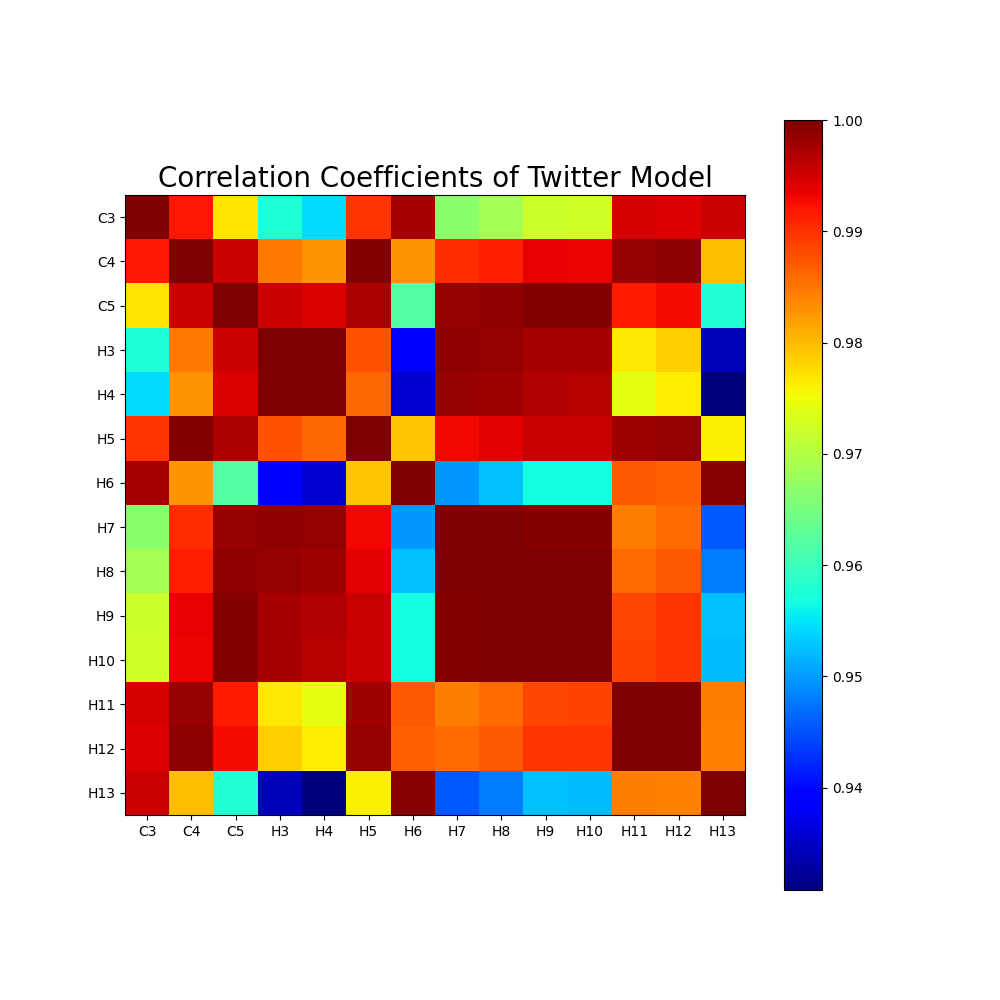
\includegraphics[width=8cm]{Images/CorrCoefTwitterModel020209.png}\
    \centering
    \caption{$\lambda=0.2$ and $p=0.2$. We recall low $\lambda$ reduces the chance of only adding a new node (T1)
    and low $p$ reduces the chance of adding a new node and a new edge. Thus 
    probabilistically this simulation should be overall adding only edges between existing nodes.}
\end{figure}

\begin{figure}
    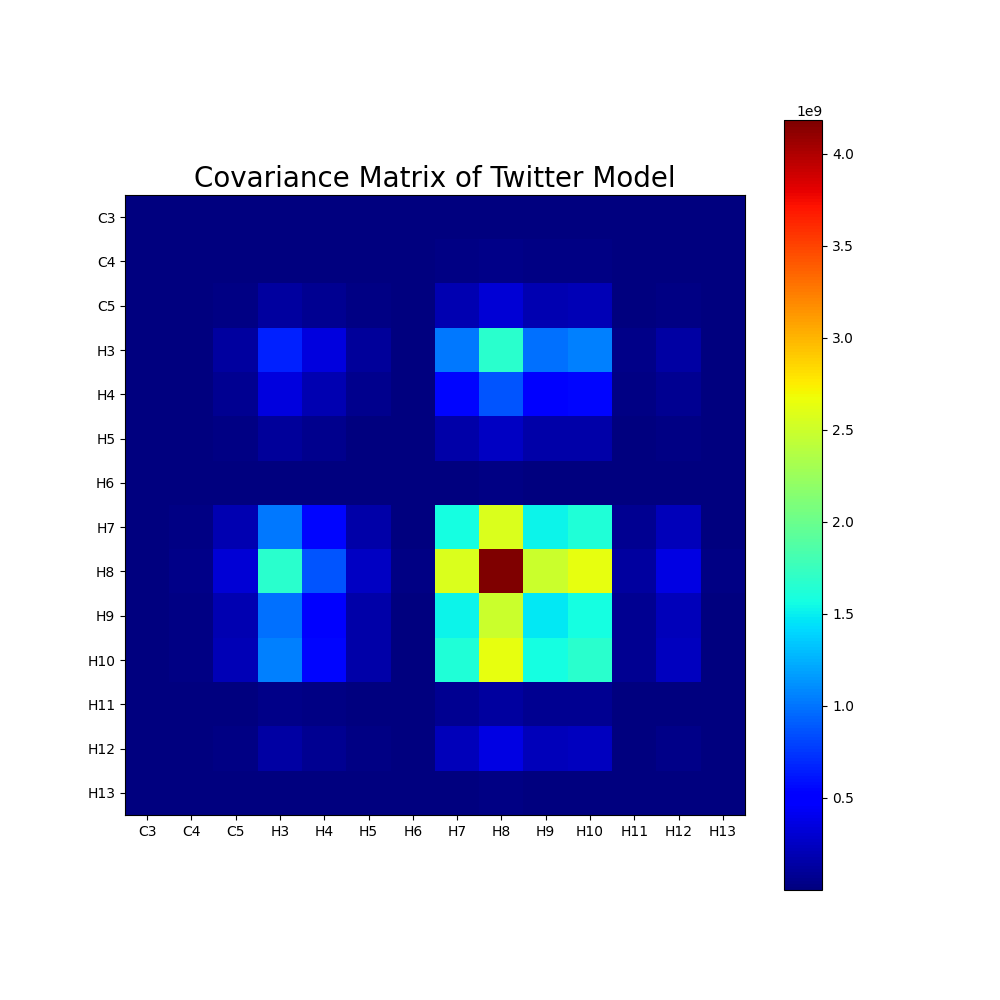
\includegraphics[width=08cm]{Images/CovMatTwitterModel020209.png}\
    \centering
    \caption{$\lambda=0.2$ and $p=0.2$. Here we see once again 
    a strong covariance relationship between H7,H8,H9,H10. In this particular graph 
    it's insightful to see these traveling together given these parameters 
    are less likely to produce the induced star subgraph we expect to see for higher $p$.}
\end{figure}

\begin{figure}
    \includegraphics[width=08cm]{Images/CorrCoefTwitterModel020809.png}\
    \centering
    \caption{$\lambda=0.2$ and $p=0.8$. Here in the correlation coeffecients we 
    see that there is still strong correlation between H7,H8, but otherwise a much
    larger spread over the motifs. We also see that no H6 or H13 motifs appeared
    throughout this simulation.}
\end{figure}

\begin{figure}
    \includegraphics[width=08cm]{Images/CovMatTwitterModel020809.png}\
    \centering
    \caption{$\lambda=0.2$ and $p=0.8$. Here the covariance is realtively 
    very small, except for the H4 variance. This is suggestive of the 
    the high $p$ generating that induced star subgraph.}
\end{figure}

\begin{figure}
    \includegraphics[width=08cm]{Images/CorrCoefTwitterModel080209.png}\
    \centering
    \caption{$\lambda=0.8$ and $p=0.2$. Once again we see a familiar structure
    in the correlation matrix. Here though we do see strong correlations 
    across a wider selection of motifs: C3,C4,C5,H3,H4,H5,H7,H8,H9,H10. It appears
    the H6's are not easily produced by any of the parameters chosen or the 
    Barabási–Albert model.}
\end{figure}

\begin{figure}
    \includegraphics[width=08cm]{Images/CovMatTwitterModel080209.png}\
    \centering
    \caption{$\lambda=0.8$ and $p=0.2$. We do see strong covariance around the $H4$ with 
    other motifs. There is possibly multiple induced star subgraphs connected that could
    drive this phenomena generating many H4's along with other motifs.}
\end{figure}

\begin{figure}
    \includegraphics[width=08cm]{Images/CorrCoefTwitterModel080809.png}\
    \centering
    \caption{$\lambda=0.8$ and $p=0.8$. Here we have a higher likelihood of adding a new node
    or a new edge and node. Here we do not see any new H6's or H8's produced after the initializtion of 
    the graph. Any block structures that we saw in earlier correlation matrices are not as apparent, although
    there is still strong H7-H8 correlation. }
\end{figure}

\begin{figure}
    \includegraphics[width=08cm]{Images/CovMatTwitterModel080809.png}\
    \centering
    \caption{$\lambda=0.8$ and $p=0.8$. The covariances fromed by this simulation suggest once again
    an overlapping of H4's, but there are clearly more nodes attached to the outer edges of this
    induced subgraph. This could lead to the covariance we see between H4 and H3}
\end{figure}

\FloatBarrier

Above we can see clearly evidence of the $S_k$, $k>>1$ induced subgraph
for high values of $p$. We see relatively high covariance between the $H7's$ amd
$H8's$ and with $H3$ and $H3$. $H13$ and $H6$ counts don't change at all because the probablity
of $T2$ attachment through the superstar mechanism is high relatively high. In fact this 
mechanism is what encourages the growth of those motifs we expect to grow combinatorially 
around $S_k$ induced subgraphs.

\chapter{Dynamic Mode Decomposition}

\section{The Koopman Operator}


Suppose we have some finite-dimensional, but non-linear system 

$$
\frac{dy}{dt} = f(y) \quad y(0) = x \in \mathbb{R}^N
$$

with $N>>1$. Furtheremore we can define the associated flow $y(t)$
as 

$$
y(t) = \phi(t;x)
$$

We also define a Hilbert Space of observables, that is 

$$
L_2(O) = L_2(\mathbb{R}^N, \mathbb{R}, \mu)
$$

with an assoicated norm 

$$
\int_{\mathbb{R}^N} |g(x) |^2 d\mu(x)  < \infty
$$

and $/mu$ is some appropriately chosen measure. We introduce the Koopman
operator $K$, a mapping between the Hilbert space of observables unto itself,

$$
K: L_2(O) \rightarrow L_2(O)
$$

$$
Kg(x) = g(\phi(x)) \quad g \in L_2(O)
$$

The movement from a non-linear dynamical system to a linear operator allows us
to capture the dynamics of the system simply by examining the eigenvalues of 
that linear operator $K$. Now suppose that $K$ only has discrete spectra. We can then find a basis of 
$L_2(O)$ through the Koopman eigenfucntions $\xi$, then it follows
%cite that other other things chris sent you.

$$
K^t \xi_j = e^{t\lambda_j}\xi_j
$$

Then for any observable $g$ we have

$$
g = \sum^{\infty}_{j=1} c_j \xi_j = \sum^{\infty}_{j=1} e^{t\lambda_j}c_j\xi_j
$$

However finding the exact eigenfucntions and eigenvalues of $K$ analytic
is difficult for any meaningful problem, and thus we hae to resort to
numerics to estimate them via the Dynamic Mode Decomposition.


\section{Finding the Koopman Operator via Dynamic Mode Decomposition}

We begin by considering data collected from what we suspect is a non-linear dynamical system
of the form:

$$
\frac{dx}{dt} = f(x,t; \mu)
$$

where $x(t)\in \mathbb{R}^{n}$ is a vector representing the state of the dynamical system
at time $t$, and $\mu$ is our parameters. Our data is sampled at discrete points in time
say every $\Delta t$. Each sampling can be written as $x_{k} = x(k \Delta t)$. This 
discrete time-flow map we denote $X_{k+1} = F(x_k)$.Collecting measurements of the system at each time step
we write:

$$
y_k = g(x_k)
$$

where $g(k)$ is the set of observables formed from the state space. 
Here we now use the Koopman operator theory to introduce a
 linear infinite-dimensional operator ${\hat K }$ such that:

$$
K g = K g(x_k) =g \circ F = g(F(x_k)) = g(x_{k+1})
$$

Thus the Koopman operator $K$ advances measurements along the flow $F$ by $\Delta t$.
We calculate the Koopman operator of our respective dynamical system as follows:

We begin with our data snapshot matrix composed of the relevant observables:

$$
G = [g(x_0), g(x_1), g(x_2), \dots g(x_n)] = [g_1,g_2,\dots, g_n]
$$

Which we can then break into:

\begin{align*}
    & G_+ = [g_1, g_2, g_3, \dots g_n]\\
    & G_- = [g_0, g_1, g_2, \dots g_{n-1}]\\\
\end{align*}


The particular Koopman operator ${\hat K }$ we wish to find satisifies:

$$
G_+ = {\hat K}G_-
$$

It's plain to see:

$$
G_+ - {\hat K}G_- = 0
$$

$$
{\hat K } = {\argmin_{A}} \|G_+ - {A}G_- \|_{F}
$$

where $\| \|_{F}$ denotes the Frobenius norm. We still have the matter of finding the 
$A$ that minimizes the norm, and is thus our best approxmation to ${\hat K}$. 

It follows:

\begin{align*}
    G_+ &= AG_- \\
    &= AUSV^{T} \quad \text{by singular value decomposition} \\ 
U^T G_+ V S^{1} &= U^T A U \\
\end{align*}

Thus the left-hand side is related to the Koopman operator approximation $A$ via a singularity transform. Therefore the 
left-hand side and $A$ share the same eigenvalues $\lambda_i$. The eigenvectors of $U$, $\xi_i$, is a DMD mode given that
$U^T X_+ V S^{-1} \xi = \lambda_i \xi_i$. That is $\xi_i$ is an eigenvector of the left-hand side. \cite{chris}

\vspace{3mm}

Once we have approximations to the eigenfunctions and the eigenvalues we can begin to look to which modes
"contribute the most" throughout the snapshot matrix and the associated eigenvalues which describe
their temporal behavior: growth, decay, or oscillation. It should be noted that we have not yet 
discussed at all how to choose $g$ or how we build our dictonary of observables. If we choose g to 
be the identity mapping, then the method reduces to the standard DMD algorithim, where $g(x_i) = x_i$.
Choosing any other function of $g$ in a meaningful way requires some a-priori knowledge of the system.
A mapping $g$ may extend the dictionary of the observables beyond the state space and products of 
the state variables. This is aptly called Extended Dynamic Mode Decomposition (EDMD). \cite{doi:10.1137/1.9781611974508} A quick example of such
a choice might be:

$$
Y = \{y_1, y_2, y_3, \dots, y_n  \}, \quad y_i \in \mathbb{R}^{N}
$$

with 

$$
y_i = {y_{i,1}, y_{i,2},\dots, y_{i,N}} 
$$

then we might take $g$ such that:

$$
G(Y) = \{g(y_1), g(y_2), g(y_3), g(y_4), \dots , g(y_n)\}
$$

$$
g(y_i) = {y_{i,1}, y_{i,2},\dots, y_{i,N}, y^{2}_{i,1}, y_{i,1}y_{i,2}, \dots, y^{2}_{i,N}} 
$$

This example is but, one of many possible functions.

\section{Kernel Dynamic Mode Decomposition}

EDMD can very quickly generate a large set of observables
and the computational complexity of the problem increases rapidly. It suffers from the 
dimensionality problem and only works well provided many more snapshots than state space
variables. In the case we have few snapshots we introduce Kernel Dynamic Mode Decomposition,
which uses the kernel trick to overcome the curse of dimensionality\cite{doi:10.1137/1.9781611974508}. 
Thus we introduce the notion of the kernel.

\begin{dfn}
    We define the Kernel function $k:\mathbb{R}^n X \mathbb{R}^n \rightarrow \mathbb{R}, \quad k(x,{\hat x}) = <\phi(x), \phi({\hat x})>$.
     That is $k$ maps a pair of vectors to an inner product of observables of the data.
\end{dfn}

There are a variety of different Kernel's that we may choose from. Some of interest include:

sinc:

\vspace{3mm}

radial: 

\vspace{3mm}


polynomial:

\vspace{3mm}

This allows us to store a large amount of information in a single value. We thus generate matrices
$\Phi^+$ and $\Phi^-$. Suppose we choose the polynomial basis function and our data snapshots are as
follows:

$$
 Y = \{y_1,y_2,y_3, \dots y_n\}
$$

$$
k (y,{\hat y}) = (1 + y^T {\hat y})^p
$$

We then construct the observable matrices $Y^T_-Y_+ = \Phi^{+}$ and $Y^T Y = \Phi^{-}$

$$
\Phi^{+}_{i,j} = k(Y^{+}_{i}, Y^{-}_j)
$$

$$
\Phi^{-}_{i,j} = k(Y^{-}_{i}, Y^{-}_j)
$$

Then for every element we have a kernel between two snapshots in time. And the dimensionality of the
extended observables is not constrained by the total number of snapshots. For KDMD we finally get
our approximations to the Koopman modes in the familiar way.

$$
\Phi^{+} = {\bar A} \Phi^{-}
$$

\section{Accuracy Criterion}
For the two dimensionality reduction methods described above we must know how 
well the methods actually performed. We thus define first the one step reconstruction
error $r_o$.

$$
r_o = ||x_{i+1} - \lambda \xi x_{i} ||
$$

We also wish to know if the modes and eigenvalyes we have found are good approximations to 
Koopman modes. Let $\xi$ and $\lambda$ be an approximated Koopeman mode for the 
dynamical system $F$ and it's corresponding eigenvalue. Provided the $\xi$ and $\lambda$ are true estimates
it follows:

$$
\xi \circ F = \lambda \xi
$$

Introducing the norm of the function,$\|\|$, we would like to calculate 

$$
\frac{\| \xi \circ F - \lambda \xi \|}{\| \xi \|}
$$

However if we knew $F$ then Dynamic Mode Decomposition wouldn't be a very useful tool.
We must then estimate $F$ using a finite number of data points. We thus define
two data points $x_k \in X$ and ${\hat x_{k}} = F(x_k)$. We can now write 

$$
re_m = \frac{\sum_{k} |\xi {\hat x_{k}} - \mu \xi {x_{k}}|}{\sum_{k} |\xi x_k |}
$$

This we refer to as the mode error as it determines how faithfully the Dynamic Mode Decomposition
produces a set of modes similar to those of the Koopman Operator \cite{Williams_2015}. 

\chapter{Results}

\section{Preprocessing Data}
Dynamic Mode Decomposition is often sensitive to certain choices such as a choice of dictionary or 
noise in the data. Thus we implement several techniques to better our approximations of the Koopman
operator. First we modify the data via a Poisson process such that the events do not occure at each
snapshat, but the occurence of events occurs relative to a $\delta t$. To illustrate, suppose we have 

$$
X = [x_1,x_2,x_3,\dots, x_n]
$$

where $x_i$ describes the motif counts at $i \Delta t = t$. We then allow

$$
A = \frac{1}{2} \left( \frac{1}{\lambda} +  \psi(\lambda) \right)
$$

$$
\delta t = \min(A)
$$
Where $\psi(\lambda)$ is a vector of samples drawn from the exponential distribution with the same number of 
time samples and $\lambda$ is the exponent of the distribution. We then distribute events in the following
way. Let ${\hat A}$ denote  a matrix that initially only contains the value $x_1$. For $k=1,2,3,\dots$ we calculate $k \delta t$. While $k\delta t < A_i$ we append $x_i$ to 
a ${\hat A}$. Thus we generate a new matrix ${\hat A}$ that now containts $n = \sum^{N}_{i=1} A_i \mod(\delta t)$ 
snapshots where the interval of times between events are distributed according a Poisson process. Thus acts as a 
sort of smoothing of the data while also distributing the events in a 'natural' mannner. 

\vspace{3mm}

Another consideration is to center the data about the mean. This has been shown to be effective in
approximating the Koopman modes. Lastly we also normalize the data by the respect covariances 
and then compute the approximated Koopman modes. To visualize the modes on the previous scale 
one must only multiple by the respective covariances. 


\section{DMD: Barabási–Albert m=1}
We now reach a crescendo, the results of the Dynamic Mode Decomposition algorithim as applied to the
motif counts of simulated networks. The results will be separated into two parts: DMD and KDMD. We will examine the base case first, DMD as applied to the 
Barabási–Albert motif counts. Thereafter we will examine several parameter choices for the Thij model,
and then look at the distribution of eigenvalues across many parameter choices. Below the Koopman modes
and eigenvalues are as discussed above. The phi modes are simply the weighting of each Koopman mode 
at each timestep. These tell us how much energy the respective Koopman mode contributes at a given time
step.

We can now consider DMD results of the Barabási–Albert motif counts. We show below
the $m=1$ and $m=2$ case to observe difference and similarities between the approximated 
Koopman modes and eigenvalues. 

For the $m=1$ case we know that a new node and edge will be added at everytime step. Moreover from our
correlation and covariance heatmaps above we know the the only motifs that change in the $m=1$ case 
are as such: 

\newpage

\begin{figure*}
    \includegraphics[width=10cm]{Images/poissonprocess_pref_attach_1.png}
    \centering
\end{figure*}

\begin{figure*}
    \includegraphics[width=10cm]{Images/DMDm1k300eigen-1.png}
    \centering
\end{figure*}

\begin{figure*}
    \includegraphics[width=12cm]{Images/DMDm1k300eigen-2.png}
    \centering
\end{figure*}

\clearpage

\section{KDMD: Barabási-Albert m=1}

We now examine the same simulations through the KDMD method.

\FloatBarrier

\begin{figure*}
    \includegraphics[width=10cm]{Images/KDMDm1k300eigen-1.png}
    \centering
\end{figure*}

\begin{figure*}
    \includegraphics[width=12cm]{Images/KDMDm1k300eigen-2.png}
    \centering
\end{figure*}

\clearpage

\FloatBarrier

\section{DMD: Barabási–Albert m=2}

\begin{figure*}
    \includegraphics[width=12cm]{Images/poissonprocess_pref_attach_2.png}
    \centering
\end{figure*}

\begin{figure*}
    \includegraphics[width=10cm]{Images/DMDm2k300eigen-1.png}
    \centering
\end{figure*}

\begin{figure*}
    \includegraphics[width=12cm]{Images/DMDm2k300eigen-2.png}
    \centering
\end{figure*}

\clearpage

\section{KDMD: Barabási–Albert m=2}

\begin{figure*}
    \includegraphics[width=10cm]{Images/KDMDm2k300eigen-1.png}
    \centering
\end{figure*}

\begin{figure*}
    \includegraphics[width=12cm]{Images/KDMDm2k300eigen-2.png}
    \centering
\end{figure*}

\clearpage

\section{DMD: Thij with $\lambda=0.2$, $p=0.2$}
\begin{figure*}
    \includegraphics[width=12cm]{Images/twitter_counts_020209.png}
    \centering
\end{figure*}


\begin{figure*}
    \includegraphics[width=10cm]{Images/DMD_twitter_020209-1.png}
    \centering
\end{figure*}

\begin{figure*}
    \includegraphics[width=12cm]{Images/DMD_twitter_020209-2.png}
    \centering
\end{figure*}

\section{KDMD: Thij with $\lambda=0.2$, $p=0.2$}

\FloatBarrier


\begin{figure*}
    \includegraphics[width=10cm]{Images/KDMD_twitter_020209-1.png}
    \centering
\end{figure*}

\begin{figure*}
    \includegraphics[width=12cm]{Images/KDMD_twitter_020209-2.png}
    \centering
\end{figure*}

\FloatBarrier
\section{DMD: Thij with $\lambda=0.2$, $p=0.8$}
\begin{figure*}
    \includegraphics[width=12cm]{Images/twitter_counts_020809.png}
    \centering
    \caption{Motif counts for Thij model with $\lambda=0.2$,$p=0.8$.}
\end{figure*}

\begin{figure*}
    \includegraphics[width=10cm]{Images/DMD_twitter_020809-1.png}
    \centering
    \caption{Approximated eigenvalues by DMD for Thij model
    with $\lambda=0.2$,$p=0.8$.}
\end{figure*}

\begin{figure*}
    \includegraphics[width=12cm]{Images/DMD_twitter_020809-2.png}
    \centering
    \caption{Approximated Koopman modes by DMD for Thij model
    with $\lambda=0.2$,$p=0.8$.}
\end{figure*}


\section{KDMD: Thij with $\lambda=0.2$, $p=0.8$}


\begin{figure*}
    \includegraphics[width=10cm]{Images/KDMD_twitter_020809-1.png}
    \centering
    \caption{Approximated eigenvalues by KDMD for Thij model
    with $\lambda=0.2$,$p=0.8$.}
\end{figure*}

\begin{figure*}
    \includegraphics[width=12cm]{Images/KDMD_twitter_020809-2.png}
    \centering
    \caption{Approximated eigenvalues by KDMD for Thij model
    with $\lambda=0.2$,$p=0.8$.}
\end{figure*}

\FloatBarrier

\section{DMD: Thij with $\lambda=0.4$, $p=0.4$}

\begin{figure*}
    \includegraphics[width=12cm]{Images/twitter_counts_040409.png}
    \centering
\end{figure*}

\begin{figure*}
    \includegraphics[width=10cm]{Images/DMD_twitter_040409-1.png}
    \centering
    \caption{Approximated eigenvalues by DMD for Thij model
    with $\lambda=0.4$,$p=0.4$.}
\end{figure*}

\begin{figure*}
    \includegraphics[width=12cm]{Images/DMD_twitter_040409-2.png}
    \centering
    \caption{Approximated Koopman modes by DMD for Thij model
    with $\lambda=0.4$,$p=0.4$.}
\end{figure*}
 

\clearpage

\section{KDMD: Thij with $\lambda=0.4$, $p=0.4$}

\begin{figure*}
    \includegraphics[width=10cm]{Images/KDMD_twitter_040409-1.png}
    \centering
    \caption{Approximated eigenvalues by KDMD for Thij model
    with $\lambda=0.4$,$p=0.4$.}
\end{figure*}

\begin{figure*}
    \includegraphics[width=12cm]{Images/KDMD_twitter_040409-2.png}
    \centering
    \caption{Approximated Koopman modes by KDMD for Thij model
    with $\lambda=0.4$,$p=0.4$.}
\end{figure*}


\FloatBarrier

\clearpage

\section{DMD: Thij with $\lambda=0.8$, $p=0.2$}
\begin{figure*}
    \includegraphics[width=12cm]{Images/twitter_counts_080209.png}
    \centering
    \caption{Motif counts for Thij simulation with $\lambda=0.8$,$p=0.2$}
\end{figure*}

\begin{figure*}
    \includegraphics[width=10cm]{Images/DMD_twitter_080209-1.png}
    \centering
    \caption{Approximated eigenvalues by DMD for Thij model
    with $\lambda=0.8$,$p=0.2$.}
\end{figure*}

\begin{figure*}
    \includegraphics[width=12cm]{Images/DMD_twitter_080209-2.png}
    \centering
    \caption{Approximated Koopman modes by DMD for Thij model
    with $\lambda=0.8$,$p=0.2$.}
\end{figure*}


\clearpage
\section{KDMD: Thij with $\lambda=0.8$, $p=0.2$}


\begin{figure*}
    \includegraphics[width=10cm]{Images/KDMD_twitter_080209-1.png}
    \centering
    \caption{Approximated eigenvalues by KDMD for Thij model
    with $\lambda=0.8$,$p=0.2$.}
\end{figure*}

\begin{figure*}
    \includegraphics[width=12cm]{Images/KDMD_twitter_080209-2.png}
    \centering
    \caption{Approximated Koopman modes by KDMD for Thij model
    with $\lambda=0.8$,$p=0.2$.}
\end{figure*}

\FloatBarrier

\clearpage

\section{DMD: Thij with $\lambda=0.8$, $p=0.8$}
\begin{figure*}
    \includegraphics[width=12cm]{Images/twitter_counts_080809.png}
    \centering
    \caption{Motif counts for Thij model with $\lambda=0.8$,$p=0.8$.}
\end{figure*}

\begin{figure*}
    \includegraphics[width=10cm]{Images/DMD_twitter_080809-1.png}
    \centering
    \caption{Approximated eigenvalues by DMD for Thij model
    with $\lambda=0.8$,$p=0.8$.}
\end{figure*}

\begin{figure*}
    \includegraphics[width=12cm]{Images/DMD_twitter_080809-2.png}
    \centering
    \caption{Approximated Koopman modes by DMD for Thij model
    with $\lambda=0.8$,$p=0.8$.}
\end{figure*}

\section{KDMD: Thij with $\lambda=0.8$, $p=0.8$}

\begin{figure*}
    \includegraphics[width=10cm]{Images/KDMD_twitter_080809-1.png}
    \centering
    \caption{Approximated eigenvalues by KDMD for Thij model
    with $\lambda=0.8$,$p=0.8$.}
\end{figure*}

\begin{figure*}
    \includegraphics[width=12cm]{Images/KDMD_twitter_080809-2.png}
    \centering
    \caption{Approximated Koopman modes by KDMD for Thij model
    with $\lambda=0.8$,$p=0.8$.}
\end{figure*}

\FloatBarrier


\section{Accuracy of Methods}

We obviously want to know how DMD handles different parameter simulations of the Thij model,
but also how it compares to KDMD. We also need to evaluate how the two accruacy criterion vary across
simulations and methods. 

For mode error each error is for a particular approximated mode. We begin with the mode error of the 
Barabási–Albert models.

\begin{table}
    \centering
    \begin{tabular}{||c c c ||} 
    \hline
    Params & DMD & KDMD  \\ [0.5ex] 
    \hline\hline
    $m=1$ & 2.25e-03 &  1.19e+00\\ 
    \hline
    $m=2$ & 3.70e-03 & 2.00e+01 \\
    \hline
   \end{tabular}
   \caption{One-step Errors of the DMD and KDMD methods on the Barabási–Albert model with $m=1$ and $m=2$}
   \label{table:15}
\end{table}

\begin{figure}
    \includegraphics[width=8cm]{Images/mode_error_dmd_prefattach1.png}
    \centering
    \caption{DMD Mode error for preferential attachment with $m=1$}
\end{figure}

\begin{figure}
    \includegraphics[width=8cm]{Images/mode_error_kdmd_prefattach1.png}
    \centering
    \caption{KDMD Mode error for preferential attachment with $m=1$}
\end{figure}

\begin{figure}
    \includegraphics[width=8cm]{Images/mode_error_dmd_prefattach2.png}
    \centering
    \caption{KDMD Mode error for preferential attachment with $m=2$}
\end{figure}

\begin{figure}
    \includegraphics[width=8cm]{Images/mode_error_kdmd_prefattach2.png}
    \centering
    \caption{KDMD Mode error for preferential attachment with $m=2$}
\end{figure}

\FloatBarrier

We still need to consider performance on the more complex Thij model.


\begin{table}
    \centering
    \begin{tabular}{||c c c ||} 
    \hline
    $(\lambda,p)$ & DMD & KDMD  \\ [0.5ex] 
    \hline\hline
    $(0.2,0.2)$ & 1.25e-03 &  5.57e-01\\ 
    \hline
    $(0.4,0.4)$ & 3.38e-03 & 9.16e-01 \\
    \hline
    $(0.2,0.8)$ & 7.37e-03 & 2.63e+00 \\
    \hline
    $(0.8,0.2)$ & 4.14e-03 & 8.98e-01\\
    \hline
    $(0.8,0.8)$ & 6.74e-03 &  5.24e-02 \\
    \hline
   \end{tabular}
   \caption{One-step Errors of the DMD and KDMD methods on the Thij model.
   DMD generally performs better than KDMD in reconstruction errors.}
   \label{table:15}
\end{table}

Now we can evalute the respective mode errors.

\begin{figure}
    \includegraphics[width=8cm]{Images/mode_error_dmd_twitter_020209.png}
    \centering
    \caption{DMD mode error for Thij model $(0.2,0.2,0.9)$}
\end{figure}

\begin{figure}
    \includegraphics[width=8cm]{Images/mode_error_kdmd_twitter_020209.png}
    \centering
    \caption{KDMD mode error for Thij model $(0.2,0.2,0.9)$}
\end{figure}


\begin{figure}
    \includegraphics[width=8cm]{Images/mode_error_dmd_twitter_040409.png}
    \centering
    \caption{DMD mode error for Thij model $(0.4,0.4,0.9)$}
\end{figure}


\begin{figure}
    \includegraphics[width=8cm]{Images/mode_error_kdmd_twitter_040409.png}
    \centering
    \caption{KDMD mode error for Thij model $(0.4,0.4,0.9)$}
\end{figure}


\begin{figure}
    \includegraphics[width=8cm]{Images/mode_error_dmd_twitter_020809.png}
    \centering
    \caption{DMD mode error for Thij model $(0.2,0.8,0.9)$}
\end{figure}


\begin{figure}
    \includegraphics[width=8cm]{Images/mode_error_kdmd_twitter_020809.png}
    \centering
    \caption{KDMD mode error for Thij model $(0.2,0.8,0.9)$}
\end{figure}


\begin{figure}
    \includegraphics[width=8cm]{Images/mode_error_dmd_twitter_080209.png}
    \centering
    \caption{DMD mode error for Thij model $(0.8,0.2,0.9)$}
\end{figure}


\begin{figure}
    \includegraphics[width=8cm]{Images/mode_error_kdmd_twitter_080209.png}
    \centering
    \caption{KDMD mode error for Thij model $(0.8,0.2,0.9)$}
\end{figure}

\begin{figure}
    \includegraphics[width=8cm]{Images/mode_error_dmd_twitter_080809.png}
    \centering
    \caption{DMD mode error for Thij model $(0.8,0.8,0.9)$}
\end{figure}


\begin{figure}
    \includegraphics[width=8cm]{Images/mode_error_kdmd_twitter_080809.png}
    \centering
    \caption{KDMD mode error for Thij model $(0.8,0.8,0.9)$}
\end{figure}

\FloatBarrier

From examining these mode errors we can see that generally the modes
from the standard DMD algorithim are just as accurate, if not more 
than the KDMD modes. DMD also performs much better in terms of one-step
reconstruction than KDMD, which is not unexpected since 
DMD is effectively a least-squares fit to the data. Overall given that 
DMD is more accurate in this context, and that KDMD rquires much
more resources DMD seems to be the better tool.


\chapter{Discussion}
We see from the results above that are able to sleuce out different in dynamic behavior from applying
the Dynamic Mode Decomposition to the motif counts. The modes themselves are not orthogonal so they
may not necessarily be picking out modes that are uncorrelated as principle componenet analysis might. 
However each mode is associated with a dynamic behavior. Given that certain counts grow exponentially 
fast certain modes obviously pick out and are associated with those features.


We also see above the DMD will still generate modes that are orthogonal provided that
one of the motif counts never changes over time. The associated eigenvalue of those modes are zero,
and thus that mode doesn't contribute to the dynamic development. KDMD will not 
pick out orthogonal modes, but will just produce modes of dimension equal to the number of counts evolving
over time, a consequence of the manner in which KDMD is implemented.


For certain simulations we have a readily available a-priori explanation
of the dynamics, the formation of large induced star subgraphs. The preferential
attachment mechanism effectively acts as a positive feedback loop - the
additional attachment of nodes to a node $u$ increasing
the likelihood of the future attachment to node $u$. Even without 
the such a tale DMD and KDMD are a capable of extracting out underlying 
structure from those simultations which do not exhibit the same pattern
for example a Thij model with $\lambda=0.8$,$p=2$ or $\lambda=0.8$,$p=0.8$.
There is for any of the given simulations a handful of DMD or KDMD modes that 
have relatively low error. 



\chapter{Conclusion}

Using these data driven methods we are clearly able to pick out underlying structure in the motif
counts using DMD or KDMD. It may be possible upon further study to use
DMD or KDMD to classify networks based upon their dynamical behavior
by examining their modes or their eigenvalues. For instance above
we discuss the impact Twitter has had on modern politicals and the 
prevalance of bots in spreading misinformation across Twitter. DMD or KDMD
might show differences between those users which are human and those are 
bots. DMD may also offer a different way of classifying those users 
which are truly influential on Twitter, different from follower count or
retweet count, but a way of temporal classification grounded in networks.

